\chapter{Methods}

% %%%%% COME BACK TO THIS TO SEE IF I CAN ADD SOMETHING ABOUT THE MERG
% \section{The Unitary renormalisation group method}
% The URG method was introduced and formalised in refs.~\cite{anirbanurg1,anirbanurg2,anirbanmott1,anirbanmott2}.  This section is adapted from those references and expanded wherever required.
% \subsection*{Description of the problem}
% We are given a Hamiltonian \(\mathcal{H}\) which is not completely diagonal in the occupation number basis of the electrons, \(\hat n_k\): \(\left[\mathcal{H},n_k\right] \neq 0\). \(k\) labels any set of quantum numbers depending on the system. For spin-less Fermions it can be the momentum of the particle, while for spin-full Fermions it can be the set of momentum and spin. There are terms that scatter electrons from one quantum number \(k\) to another quantum number \(k^\prime\).
%
% We take a general Hamiltonian,
% \begin{equation}\begin{aligned}
% 	\mathcal{H} = H_e \hat n_{q\beta} + H_h \left(1 - \hat n_{q\beta}\right) + c^\dagger_{q\beta}T + T^\dagger c_{q\beta}
% \end{aligned}\end{equation}
% Formally, we can decompose the entire Hamiltonian in the subspace of the electron we want to decouple (\(q\beta\)).
% \begin{equation}\begin{aligned}
% 	\label{matham}
% \mathcal{H} = \bordermatrix{~ & \ket{1} & \ket{0} \cr
%               & H_1 & T \cr
%               & T^\dagger & H_0 \cr}
% \end{aligned}\end{equation}
% The basis in which this matrix is written is \(\left\{\ket{1},\ket{0}\right\}\) where \(\ket{i}\) is the set of all states where \(\hat n_{q\beta}=i\). The aim of one step of the URG is to find a unitary transformation \(U\) such that the new Hamiltonian \(U \mathcal{H} U^\dagger\) is diagonal in this already-chosen basis.
% \begin{equation}\begin{aligned}
% 	\tilde{\mathcal{H}} \equiv U \mathcal{H} U^\dagger = \bordermatrix{~ & \ket{1} & \ket{0} \cr
%               & \tilde H_1 & 0 \cr
%               & 0 & \tilde H_0 \cr}
% \end{aligned}\end{equation}
% \(U_q\) is defined by
% \begin{equation}\begin{aligned}
% 	\tilde{\mathcal{H}} = U_q \mathcal{H} U^\dagger_q \text{   such that  } \left[\tilde{\mathcal{H}},n_q\right] = 0
% \end{aligned}\end{equation}
% It is clear that \(U\) is the diagonalizing matrix for \(\mathcal{H}\). Hence we can frame this problem as an eigenvalue equation as well. Let \(\ket{\psi_1},\ket{\psi_0}\) be the basis in which the original Hamiltonian \(\mathcal{H}\) has no off-diagonal terms corresponding to \(q\beta\). Hence, we can write
% \begin{equation}\begin{aligned}
% 	\label{diageq}
%     \mathcal{H} \ket{\psi_i} = \tilde H_i\ket{\psi_i}, i\in\left\{0,1\right\}
% \end{aligned}\end{equation}
% Since \(\ket{\psi_i}\) is the set of eigenstates of \(\mathcal{H}\) and \(\ket{i}\) is the set of eigenstates in which \(U\mathcal{H} U^\dagger\) has no off-diagonal terms corresponding to \(q\beta\), we can relate \(\ket{\psi_i}\) and \(\ket{i}\) by the same transformation : \(\ket{\psi_i} = U^\dagger\ket{i}\). We can expand the state \(\ket{\psi_i}\) in the subspace of \(q\beta\):
% \begin{equation}\begin{aligned}
% 	\label{matpsi}
% \ket{\psi_i} = \sum_{j=0,1} \ket{j}\bra{j}\ket{\psi_i} \equiv \ket{1}\ket{\phi_1^i} + \ket{0}\ket{\phi_0^i}\end{aligned}\end{equation}
% where \(\ket{\phi_j^i} = \bra{j}\ket{\psi_i}\). If we substitute the expansion \ref{matham} into the eigenvalue equation \ref{diageq}, we get
% \begin{equation}\begin{aligned}
% 	\left[H_e \hat n_{q\beta} + H_h \left(1 - \hat n_{q\beta}\right) + c^\dagger_{q\beta}T + T^\dagger c_{q\beta}\right]\ket{\psi_i} = \tilde H_i\ket{\psi_i}
% \end{aligned}\end{equation}
% The diagonal parts \(H_e = \text{tr}\left[\mathcal{H} \hat n_{q\beta}\right]\) and \(H_e = \text{tr}\left[\mathcal{H} \left(1 - \hat n_{q\beta}\right)\right]\) can be separated into a purely diagonal part \(\mathcal{H}^d\) that contains the single-particle energies and the multi-particle correlation energies or Hartree-like contributions, and an off-diagonal part  \(\mathcal{H}^i\) that scatters between the remaining degrees of freedom \(k\sigma \neq q\beta\). That is,
% \begin{equation*}
% \begin{gathered}
% 	H_e \hat n_{q\beta} + H_h \left(1 - \hat n_{q\beta}\right) = \mathcal{H}^d + \mathcal{H}^i\\
% \end{gathered}
% \end{equation*}
% This gives
% \begin{equation}\begin{aligned}
% 	\left[c^\dagger_{q\beta}T + T^\dagger c_{q\beta}\right]\ket{\psi_i} = \left(\tilde H_i - \mathcal{H}^i - \mathcal{H}^d\right)\ket{\psi_i}
% \end{aligned}\end{equation}
% \subsection*{Obtaining the decoupling transformation}
% We now define a new operator \(\hat \omega_i = \tilde H_i - \mathcal{H}^i\), such that 
% \begin{equation}\begin{aligned}
% 	\left[c^\dagger_{q\beta}T + T^\dagger c_{q\beta}\right]\ket{\psi_i} = \left(\hat \omega_i - \mathcal{H}^d\right)\ket{\psi_i}
% \end{aligned}\end{equation}
% From the definition of \(\hat \omega_i\), we can see that it is Hermitian and has no term that scatters in the subspace of \(q\beta\), so it is diagonal in \(q\beta\) and we can expand it as \(\hat \omega_i = \hat \omega_i^1 \hat n_{q\beta} + \hat \omega_i^0 \left(1 - \hat n_{q\beta}\right)\). Using the expansion \ref{matpsi}, we can write
% \begin{equation}\begin{aligned}
% \hat \omega_i \ket{\psi_i} = \hat \omega_i^1 \ket{1}\ket{\phi_1^i} + \hat \omega_i^0 \ket{0}\ket{\phi_0^i}
% \end{aligned}\end{equation}
% Since the only requirement on \(\ket{\psi_i}\) is that it diagonalize the Hamiltonian in the subspace of \(q\beta\), there is freedom in the choice of this state. We can exploit this freedom and choose the \(\ket{\phi_{0,}^i}\) to be an eigenstates of \(\hat \omega_i^{1,0}\) corresponding to real eigenvalues \(\omega_i^{1,0}\):
% \begin{equation}\begin{aligned}
% 	\left[\mathcal{H}^d + c^\dagger_{q\beta}T + T^\dagger c_{q\beta}\right]\ket{\psi_i(\omega_i)} = \left(\omega_i^1 - \mathcal{H}^d\right)\ket{1}\ket{\phi_1^i} + \left(\omega_i^0 - \mathcal{H}^d\right)\ket{0}\ket{\phi_0^i}
% \end{aligned}\end{equation}
% If we now substitue the expansion \ref{matpsi} and gather the terms that result in \(\hat n_{q\beta}=1\), we get
% \begin{equation}\begin{aligned}
% 	\label{changea}
% 	c^\dagger_{q\beta}T\ket{0}\ket{\phi_0^i} = \left(\omega_i^1 - \mathcal{H}^d\right)\ket{1}\ket{\phi_1^i}
% \end{aligned}\end{equation}
% Similarly, gathering the terms that result in \(\hat n_{q\beta}=0\) gives
% \begin{equation}\begin{aligned}
% 	\label{changeb}
% 	T^\dagger c_{q\beta}\ket{1}\ket{\phi_1^i} = \left(\omega_i^0 - \mathcal{H}^d\right)\ket{0}\ket{\phi_0^i}
% \end{aligned}\end{equation}
% We now define two many-particle transition operators:
% \begin{equation}\begin{aligned}
% 	\label{etadefine}
% {\eta}^\dagger(\omega_i^1) = \frac{1}{\omega_i^1- \mathcal{H}^d}c^\dagger_{q\beta}T \equiv G_1 c^\dagger_{q\beta}T\\
% \eta(\omega_i^0) = \frac{1}{\omega_i^0- \mathcal{H}^d}T^\dagger c_{q\beta} \equiv G_0 T^\dagger c_{q\beta}
% \end{aligned}\end{equation}
% wher \(G_j\) is the propagator \(\frac{1}{\omega_i^j- \mathcal{H}^d}\). We can write this compactly as
% \begin{equation}\begin{aligned}
% 	\label{etadagdef}
% \eta(\hat \omega) = GT^\dagger c_{q\beta} = \frac{1}{\hat \omega_i- \mathcal{H}^d}T^\dagger c_{q\beta}
% \end{aligned}\end{equation}
% where \(\hat \omega_i = \omega_i^0\left(1 - \hat n_{q\beta}\right) + \omega_i^1\hat n_{q\beta} = \begin{pmatrix} \omega_i^1 & \\ & \omega_i^0 \end{pmatrix}\) is a 2x2 matrix and \(\mathcal{H}^d = \mathcal{H}^d_0\left(1 - \hat n_{q\beta}\right) + \mathcal{H}^d_1\hat n_{q\beta}\) and \(G = \left(\hat \omega - \mathcal{H}^d\right)^{-1}\). It is easy to check that this reproduces the previous forms of \(\eta_0\) and \(\eta_1^\dagger\).
% We will later find that it is important to demand that these two be Hermitian conjugates of each other; that constraint is imposed on the denominators:
% \begin{equation}\begin{aligned}
% 	\label{constraint}
% \eta^\dagger(\omega_i^0) = \eta^\dagger(\omega_i^1) \implies \frac{1}{\omega_i^1- \mathcal{H}^d}c^\dagger_{q\beta}T = c^\dagger_{q\beta}T\frac{1}{\omega_i^0- \mathcal{H}^d}
% \end{aligned}\end{equation}
% Henceforth we will assume that this constraint has been imposed. 
%
% In terms of these operators, eq.~\ref{changeb} becomes
% \begin{equation}\begin{aligned}
%     \ket{1}\ket{\phi_1^i} &= {\eta}^\dagger\ket{0}\ket{\phi_0^i}, ~ ~ ~\ket{0}\ket{\phi_0^i} &= \eta\ket{1}\ket{\phi_1^i}
% \end{aligned}\end{equation}
% These allow us to write
% \begin{equation}\begin{aligned}
% 	\label{trans}
% 	\ket{\psi_1} &= \ket{1}\ket{\phi_1^i} + \ket{0}\ket{\phi_0^i} = \left(1 + \eta\right)\ket{1}\ket{\phi_1^i}, ~ ~ ~\ket{\psi_0} &= \left(1 + {\eta}^\dagger\right)\ket{0}\ket{\phi_0^i}
% \end{aligned}\end{equation}
% Recalling that \(\ket{\psi_i} = U^\dagger \ket{i}\), we can read off the required transformation:
% \begin{equation}\begin{aligned}
% 	\label{Ui}
%     U_1 &= 1 + \eta
% \end{aligned}\end{equation}
%
% \begin{figure}[!htb]
% \centering
% \includegraphics[width=\textwidth]{URG_method.pdf}
% \caption{Three steps of the URG: Decompose the Hamiltonian in a \(2\times 2\) matrix, apply the unitary operator to rotate it, then repeat these steps with one of the rotated blocks.}
% \end{figure}
%
% \subsection*{Properties of the many-body transition operators}
% The operators \(\eta\) have some important properties. First is the Fermionic nature:
% \begin{equation}\begin{aligned}
% 	\eta^2 = {\eta^\dagger}^2 = 0 &&\left[{c^\dagger}^2 = c^2 = 0\right]\\
% \end{aligned}\end{equation}
% Second is:
% \begin{equation}\begin{aligned}
% 	\label{antic}
%     \ket{1}\ket{\phi_1^i} &= {\eta}^\dagger\ket{0}\ket{\phi_0^i} = \eta^\dagger \eta \ket{1}\ket{\phi_1^i} \implies \eta^\dagger \eta = \hat n_{q\beta}\\
%     \ket{0}\ket{\phi_0^i} &= \eta\ket{1}\ket{\phi_1^i} = \eta \eta^\dagger\ket{\phi_0^i}\implies \eta  \eta^\dagger= 1 - \hat n_{q\beta}
% \end{aligned}\end{equation}
% and hence the anticommutator
% \begin{equation}\begin{aligned}
% 	\label{antico}
%     \implies \left\{\eta,\eta^\dagger\right\} = 1
% \end{aligned}\end{equation}
% Note that the three equations in \ref{antic} work only when applied on the eigenstate \(\ket{\psi_i}\) and not any arbitrary state.
% \begin{equation*}
%     \begin{gathered}
%     \eta^\dagger \eta \ket{\psi_i} = \ket{1}\ket{\phi_1^i} = \hat n_{q\beta}\ket{\psi_i}\\
%     \eta\eta^\dagger \ket{\psi_i} = \ket{0}\ket{\phi_0^i} = \left(1 - \hat n_{q\beta}\right)\ket{\psi_i}\\
%     \left\{\eta^\dagger,\eta\right\}\ket{\psi_i} = \ket{\psi_i}
% \end{gathered}
% \end{equation*}
% \subsection*{Form of the unitary operators}\label{unitary-form}
% Although we have found the correct similarity transformations \(U_i\) (eqs. \ref{Ui}), we need to convert them into a unitary transformation. Say we are trying to rotate the eigenstate \(\ket{\psi_1}\) into the state \(\ket{1}\). We can then work with the transformation
% \begin{equation}\begin{aligned}
% U_1 = 1 + \eta
% \end{aligned}\end{equation}
% In this form, this transformation is not unitary. It can however be written in an exponential form:
% \begin{equation}\begin{aligned}
% U_1 = e^{\eta}
% \end{aligned}\end{equation}
% using the fact that \(\eta^2 = 0\). It is shown in ref.~\cite{suzuki1984general} that corresponding to a similarity transformation \(e^\omega\),there exists a unitary transformation \(e^G\) where
% \begin{equation}\begin{aligned}
% 	G = \tanh^{-1}\left(\omega - \omega^\dagger\right)
% \end{aligned}\end{equation}
% Applying that to the problem at hand gives
% \begin{equation}\begin{aligned}
% 	U_1^\dagger &= \exp\left\{\tanh^{-1}\left(\eta - \eta^\dagger\right)\right\}
%  \end{aligned}\end{equation}
% Let \(x = \tanh y\). Then,
% \begin{equation}\begin{aligned}
% x = \frac{e^{2y} + 1}{e^{2y} - 1} \implies y = \frac{1}{2} \log\frac{1+x}{1-x} \implies e^y = e^{\tanh^{-1}x} = \sqrt\frac{1+x}{1-x}
% \end{aligned}\end{equation}
% Therefore,
% \begin{equation}\begin{aligned}
% 	\exp\left\{\tanh^{-1}\left(\eta - \eta^\dagger\right)\right\} &= \frac{1 + \eta - \eta^\dagger}{\sqrt{\left(1 + \eta^\dagger - \eta\right)\left(1 - \eta^\dagger + \eta\right)}} = \frac{1 + \eta - \eta^\dagger}{\sqrt{1 + \left\{\eta,\eta^\dagger\right\}}} = \frac{1}{\sqrt 2}\left(1 + \eta - \eta^\dagger\right)
% \end{aligned}\end{equation}
% The \textit{unitary} operator that transforms the entangled eigenstate \(\ket{\psi_1}\) to the state \(\ket{1}\) is thus
% \begin{equation}\begin{aligned}
% 	\label{finalu}
% 	U_1 = \frac{1}{\sqrt 2}\left(1 + \eta^\dagger - \eta\right)
% \end{aligned}\end{equation}
% It can also be written as \(\exp\left\{\frac{\pi}{4}\left(\eta^\dagger - \eta\right)\right\}\) because
% \begin{equation}\begin{aligned}
% 	\exp\left\{\frac{\pi}{4}\left(\eta^\dagger - \eta\right)\right\} &= 1 + \left(\eta^\dagger - \eta\right)\frac{\pi}{4} + \frac{1}{2!}\left(\eta^\dagger - \eta\right)^2\left(\frac{\pi}{4}\right)^2 + \frac{1}{3!}\left(\eta^\dagger - \eta\right)^3\left(\frac{\pi}{4}\right)^3 + ...\\
% 							   &= 1 + \left(\eta^\dagger - \eta\right)\frac{\pi}{4} - \frac{1}{2!}\left(\frac{\pi}{4}\right)^2 - \frac{1}{3!}\left(\eta^\dagger - \eta\right)\left(\frac{\pi}{4}\right)^3 + \frac{1}{4!}\left(\frac{\pi}{4}\right)^4 + ...\\
% 							   &= \cos \frac{\pi}{4} + \left(\eta^\dagger - \eta\right)\sin\frac{\pi}{4}\\
% 							   &= \frac{1}{\sqrt 2}\left(1 + \eta^\dagger - \eta\right)
% \end{aligned}\end{equation}
% There we used
% \begin{equation}\begin{aligned}
% 	\left(\eta^\dagger - \eta\right)^2 = {\eta^\dagger}^2 + \eta^2 - \left\{\eta^\dagger,\eta\right\} = -1 &&\left[\because\eta^2 = {\eta^\dagger}^2=0\right]
% \end{aligned}\end{equation}
% and hence
% \begin{equation}\begin{aligned}
% 	\left(\eta^\dagger - \eta\right)^3 = -1\left(\eta^\dagger - \eta\right)
% \end{aligned}\end{equation}
% and so on.
% \subsection*{Effective Hamiltonian}
% We can now compute the form of the effective Hamiltonian that comes about when we apply \(U_1\) - that is - when we rotate one exact eigenstate \(\ket{\psi_1}\) into the occupied Fock space basis \(\ket{1}\). From eq.~\ref{finalu},
% \begin{equation}\begin{aligned}
% 	U_1 \mathcal{H} U_1^\dagger &= \frac{1}{2}\left(1+\eta^\dagger - \eta\right)\mathcal{H}\left(1 + \eta - \eta^\dagger\right)\\
% 				    &= \frac{1}{2}\left(1+\eta^\dagger - \eta\right)\left(\mathcal{H} + \mathcal{H}\eta - \mathcal{H}\eta^\dagger\right)\\
% 				    &=\frac{1}{2}\left(\mathcal{H}+ \mathcal{H}\eta - \mathcal{H}\eta^\dagger + \eta^\dagger \mathcal{H} + \eta^\dagger\mathcal{H}\eta - \eta^\dagger \mathcal{H}\eta^\dagger - \eta\mathcal{H} - \eta \mathcal{H} \eta + \eta \mathcal{H} \eta^\dagger\right)\\
% 				    &=\frac{1}{2}\left(\mathcal{H}^d + \mathcal{H}^i + \mathcal{H}^I + \mathcal{H}\eta - \mathcal{H}\eta^\dagger + \eta^\dagger \mathcal{H} + \eta^\dagger\mathcal{H}\eta - \eta^\dagger \mathcal{H}\eta^\dagger - \eta\mathcal{H} - \eta \mathcal{H} \eta + \eta \mathcal{H} \eta^\dagger\right)\\
% 				    &=\frac{1}{2}\left(\mathcal{H}^d + \mathcal{H}^i + \mathcal{H}^I + \left[\eta^\dagger - \eta,\mathcal{H}\right] + \eta^\dagger\mathcal{H}\eta - \eta^\dagger \mathcal{H}\eta^\dagger - \eta \mathcal{H} \eta + \eta \mathcal{H} \eta^\dagger\right)\\
% \end{aligned}\end{equation}
% In the last two lines, we expanded the Hamiltonian into the three parts \(\mathcal{H}^d,\mathcal{H}^i\) and a third piece \(\mathcal{H}^I \equiv c_{q\beta}^\dagger T + T^\dagger c_{q\beta}\).
%
% For reasons that will become apparent, we will split the terms into two groups:
% \begin{equation}\begin{aligned}
% 	\tilde{\mathcal{H}} &= \frac{1}{2}\left(\underbrace{\mathcal{H}^d + \mathcal{H}^i + \left[\eta^\dagger - \eta,\mathcal{H}\right] + \eta^\dagger\mathcal{H}\eta + \eta \mathcal{H} \eta^\dagger}_\text{group 1} + \overbrace{\mathcal{H}^I - \eta^\dagger \mathcal{H}\eta^\dagger - \eta \mathcal{H} \eta}^\text{group 2}\right)\\
% \end{aligned}\end{equation}
% Group 2 can be easily shown to be 0. Note that terms that have two \(\eta\) or two \(\eta^\dagger\) sandwiching a \(\mathcal{H}\) can only be nonzero if the intervening \(\mathcal{H}\) has an odd number of creation or destruction operators.
% \begin{equation}\begin{aligned}
% 	\label{beats}
% \eta \mathcal{H} \eta = \eta c_q^\dagger  T \eta
% \end{aligned}\end{equation}
% and
% \begin{equation}\begin{aligned}
% 	\label{tora}
% \eta^\dagger \mathcal{H}\eta^\dagger = \eta^\dagger T^\dagger c_q \eta^\dagger
% \end{aligned}\end{equation}
% Group 2 becomes
% \begin{equation}\begin{aligned}
% 	\label{group2}
% \text{group 2} = \mathcal{H}^I - \eta^\dagger T^\dagger c_q \eta^\dagger - \eta c_q^\dagger  T \eta = c^\dagger_q T + T^\dagger c_q - \eta^\dagger T^\dagger c_q \eta^\dagger - \eta c_q^\dagger  T \eta
% \end{aligned}\end{equation}
% To simplify this, we use the relation
% \begin{equation}\begin{aligned}
%  \eta c_q^\dagger  T \eta &= \frac{1}{\omega_i^0 - \mathcal{H}^d}T^\dagger c_q c_q^\dagger  T \eta\\
% 			  &= T^\dagger c_q \frac{1}{\omega_i^1 - \mathcal{H}^d}c_q^\dagger  T \eta && \left[\text{eq.~\ref{constraint}}\right]\\
% 			  &= T^\dagger c_q \eta^\dagger\eta &&\left[\text{eq.~\ref{etadagdef}}\right]\\
% 			  &= T^\dagger c_q \hat n_q &&\left[\text{eq.~\ref{antic}}\right]
% \end{aligned}\end{equation}
% which gives
% \begin{equation}\begin{aligned}
% 	\label{id1}
%  \eta c_q^\dagger  T \eta  &= T^\dagger c_q 
% \end{aligned}\end{equation}
% Taking the Hermitian conjugate of eq.~\ref{id1} gives
% \begin{equation}\begin{aligned}
% 	\label{id2}
% \eta^\dagger T^\dagger c_q \eta^\dagger = c_q^\dagger T
% \end{aligned}\end{equation}
% Substituting the expressions \ref{id1} and \ref{id2} into the expression for group 2, \ref{group2}, shows that is vanishes. This leaves us only with group 1:
% \begin{equation}\begin{aligned}
% 	\widetilde{\mathcal{H}} = \frac{1}{2}\left(\mathcal{H}^d + \mathcal{H}^i + \overbrace{\eta^\dagger\mathcal{H}\eta + \eta \mathcal{H} \eta^\dagger}^\text{group A} + \underbrace{\left[\eta^\dagger - \eta,\mathcal{H}\right]}_{group B}\right)
% \end{aligned}\end{equation}
% Group A simplifies in the following way. First note that \(\eta^\dagger \mathcal{H}^I \eta = \eta^\dagger \mathcal{H}^I \eta = 0\) must be 0 because it will involve consecutive \(c_{q\beta}\) or  consecutive \(c^\dagger_{q\beta}\). We are therefore left with the diagonal part of \(\mathcal{H}\), which is \(H_e \hat  n_{q\beta} + H_h \left(1 - \hat n_{q\beta}\right)\).
% \begin{equation}\begin{aligned}
% 	\eta^\dagger\left[H_e \hat  n_{q\beta} + H_h \left(1 - \hat n_{q\beta}\right)\right]\eta + \eta\left[H_e \hat  n_{q\beta} + H_h \left(1 - \hat n_{q\beta}\right)\right]\eta^\dagger = \eta^\dagger H_h \eta + \eta H_e \eta^\dagger
% \end{aligned}\end{equation}
% This can be shown to be equal to the diagonal part:
% \begin{equation}\begin{aligned}
% 	\text{group A} = \eta^\dagger H_h \eta + \eta H_e \eta^\dagger = H_e \hat n_{q\beta} + H_h\left(1 - \hat n_{q\beta}\right) = \mathcal{H}^d + \mathcal{H}^i
% \end{aligned}\end{equation}
% It can also be shown that
% \begin{equation}\begin{aligned}
% 	\label{group B}
% 	\text{group B} = \left[\eta^\dagger - \eta,\mathcal{H}\right] = 2\left[c^\dagger_{q\beta} T,\eta\right]
% \end{aligned}\end{equation}
% Putting it all together,
% \begin{equation}\begin{aligned}
% 	\label{final2}
% 	\tilde{\mathcal{H}}= \mathcal{H}^d + \mathcal{H}^i + \left[c^\dagger_{q\beta} T, \eta\right]
% \end{aligned}\end{equation}
% The renormalizing in the Hamiltonian is
% \begin{equation}\begin{aligned}
% 	\Delta \mathcal{H} = \tilde{\mathcal{H}}- \mathcal{H}^d - \mathcal{H}^i = \left[c^\dagger_{q\beta} T, \eta\right]
% \end{aligned}\end{equation}
% Because of eq.~\ref{group B}, it can also be written as
% \begin{equation}\begin{aligned}
% 	\label{renurg}
% 	\Delta \mathcal{H} = \frac{1}{2}\left[\eta^\dagger - \eta,\mathcal{H}_X\right] = \frac{1}{2}\left[\eta^\dagger - \eta,\mathcal{H}\right]
% \end{aligned}\end{equation}
% This form will be useful later when we make the connection with one-shot Schrieffer-Wolff transformation and CUT RG.
%
% To check that the renormalised Hamiltonian indeed commutes with \(\hat n_{q\beta}\),
% \begin{equation}\begin{aligned}
% 	\left[\widetilde{\mathcal{H}}, \hat n_{q\beta}\right] &= \left[\left[c_{q\beta}^\dagger T,\eta\right],\hat n_{q\beta}\right] =\left[c_{q\beta}^\dagger T \eta,\hat n_{q\beta}\right] - \left[\eta c_{q\beta}^\dagger T,\hat n_{q\beta}\right]\\
%                    &=c^\dagger_{q\beta} T \eta \hat n_{q\beta} - \hat n_{q\beta}c^\dagger_{q\beta} T \eta &&\left[\text{2\textsuperscript{nd} [ .
% 		   ] is 0, }\because c_{q\beta}^\dagger \hat n_{q\beta} = \hat n_{q\beta} \eta=0\right]\\
%                    &=c_{q\beta}^\dagger T \eta - c_{q\beta}^\dagger T \eta =0
% \end{aligned}\end{equation}
% \subsection*{Fixed point condition}\label{match}
% Within the URG, it is a prescription that the fixed point is reached when the denominator of the RG equation vanishes. This is equivalent to either \(\omega_i^1 = \mathcal{H}^d_1 \) or \(\omega_i^0 = \mathcal{H}^d_0 \).
% This shows that at the fixed point, one of the eigenvalues of \(\hat \omega_i\) matches the corresponding eigenvalue of the diagonal blocks. This also leads to the vanishing of the off-diagonal block, because eqs.~\ref{changea} and \ref{changeb} gives
% \begin{equation}\begin{aligned}
% 	c^\dagger_{q\beta}T\ket{0}\ket{\phi_0^i} = \left(\omega_i^1 - \mathcal{H}^d_1\right)\ket{1}\ket{\phi_1^i} = 0 \implies c^\dagger_{q\beta}T = 0
% \end{aligned}\end{equation}
% \subsection*{Multiple off-diagonal terms}
% There is a subtle assumption in the definitions eq.~\ref{etadefine}. In order for \(\eta\) to be the Hermitian conjugate of \(\eta^\dagger\), \(\mathcal{H}_d\) cannot have any information that relates to the structure of \(T\). To see why, say the total off-diagonal term is composed of two parts: \(T = T_1 + T_2\).
% \begin{equation}\begin{aligned}
% 	\eta &= \frac{1}{\omega_0 - \mathcal{H}_d}\left(T_1^\dagger + T_2^\dagger\right)c = \left[\frac{1}{\omega^0 - E^0_1} T_1^\dagger c+ \frac{1}{\omega^0 - E^0_2}T_2^\dagger c\right]\\
% 	\eta^\dagger &= \frac{1}{\omega^1 - \mathcal{H}_d}c^\dagger\left(T_1 + T_2\right) = \left[\frac{1}{\omega^1 - E^1_1}c^\dagger T_1 + \frac{1}{\omega^1 - E^1_2} c^\dagger T_2\right]\\
% \end{aligned}\end{equation}
% where \(\mathcal{H}_d T_i^\dagger c = E^0_i T_i^\dagger c\) and \(\mathcal{H}_d  c^\dagger T_i = E^1_i  c^\dagger T_i\). We can now see that in order for \(\eta = \left(\eta^\dagger\right)^\dagger\) to hold, two conditions must be met:
% \begin{equation}\begin{aligned}
% 	\omega^0 - E_1^0 = \omega^1 - E_1^1, && \omega^0 - E_2^0 = \omega^1 - E_2^1
% \end{aligned}\end{equation}
% This will not hold generally. The correct solution is to realize that each such off-diagonal term \(T_i\) will come with its own quantum fluctuation scale \(\omega_i\).
% \begin{equation}\begin{aligned}
% 	\eta &= \sum_i \frac{1}{\omega^0_i - E^0_i} T_i^\dagger c\\
% 	\eta^\dagger &= \sum_i \frac{1}{\omega^1_i - E^1_1}c^\dagger T_i
% \end{aligned}\end{equation}
% If we now impose the condition that \(\eta =  \left( \eta^\dagger \right) ^\dagger\), we get the relations
% \begin{equation}\begin{aligned}
% 	\omega^0_i - \omega^1_i = E^0_i - E^1_1
% \end{aligned}\end{equation}
% and so
% \begin{equation}\begin{aligned}
% 	\eta^\dagger - \eta &= \sum_i \frac{1}{\omega^0_i - E^0_i}\left(c^\dagger T_i - T_i^\dagger c\right)
% \end{aligned}\end{equation}
% The expression for the renormalization will not be just \(\left[c^\dagger T, \eta \right]\) in this case. That form will be non-Hermitian. The correct form is obtained from the more general form \(\left[\eta^\dagger - \eta, \mathcal{H}_X \right]\):
% \begin{equation}\begin{aligned}
% 	\Delta \mathcal{H} &= \frac{1}{2}\left[\eta^\dagger - \eta, c^\dagger T + T^\dagger c\right] = \frac{1}{2}\sum_{ij} \frac{1}{\omega^0_i - E^0_i}\left[c^\dagger T_i - T_i^\dagger c, c^\dagger T_j + T_j^\dagger c\right]\\
% 		    &= \frac{1}{2}\sum_{ij} \frac{1}{\omega^0_i - E^0_i}\left[\hat n \left(T_i T_j^\dagger + T_j T_i^\dagger \right) - \left(1 - \hat n\right)\left(T_i^\dagger T_j + T_j^\dagger T_i\right)\right]\\
% 		    &= \frac{1}{2}\sum_{ij} \left(\frac{1}{\omega^0_i - E^0_i} + \frac{1}{\omega^0_j - E^0_j}\right)\left[\hat n T_i T_j^\dagger - \left(1 - \hat n\right)T_i^\dagger T_j\right]\\ 
% \end{aligned}\end{equation}
% \subsection*{Equivalence of the two unitaries and preservation of partial trace}
% In the subsection \ref{unitary-form}, we determined the form of the operator \(U_1\) that unitarily decouples the node \(q\beta\) from the other degrees of freedom. Eq.~\ref{finalu} was derived by reading off the transformation of \(\ket{1}\) to \(\ket{\psi_1}\), the first equation in \ref{trans}. We could easily have chosen the other equation in the same equation set,
% \begin{gather*}
% 	\ket{\psi_0} = \left(1 + {\eta}^\dagger\right)\ket{0}\ket{\phi_0^i}
% \end{gather*}
% which gives a similarity  transformation \(1+\eta^\dagger\) and hence a unitary
% \begin{equation}\begin{aligned}
% 	U_0 = \frac{1}{\sqrt 2}\left(1 + \eta - \eta^\dagger\right)
% \end{aligned}\end{equation}
% This \(\eta\) will however be different from the \(\eta\) in eq.~\ref{finalu}. The reason is, in order to get \(U_1\), we must start from the eigenvalue equation \(\mathcal{H} \ket{\psi_1} = \tilde H_1 \ket{\psi_1}\). This means that the corresponding \(\hat \omega\) will be defined as \(\hat \omega_1 = \tilde H_1 - \mathcal{H}^i\). On the other hand, in order to get \(U_0\) we must start with \(\mathcal{H} \ket{\psi_0} = \tilde H_0 \ket{\psi_0}\), and hence this \(\hat \omega\) will be \(\hat \omega_0 = \tilde H_0 - \mathcal{H}^i\). This difference in the \(\hat \omega\) will define two different sets of \(\eta\):
% \begin{equation}\begin{aligned}
% 	\label{eta0}
% \text{Starting from \(\ket{\psi_1}\):	}\eta_1 = \frac{1}{\omega_1^0- \mathcal{H}^d}T^\dagger c_{q\beta} && \text{and }\eta^\dagger_1 = \frac{1}{\omega_1^1- \mathcal{H}^d}T^\dagger c_{q\beta}\\
% \text{Starting from \(\ket{\psi_0}\):	}\eta_0 = \frac{1}{\omega_0^0- \mathcal{H}^d}T^\dagger c_{q\beta} && \text{and }\eta^\dagger_0 = \frac{1}{\omega_0^1- \mathcal{H}^d}T^\dagger c_{q\beta}
% \end{aligned}\end{equation}
% The \(\omega_j^i\) eigenvalues have both upper and lower indices. The upper index \(i\) signifies which eigenstate it relates to - \(\omega_j \ket{i} = \omega_j^i\ket{i}\). The lower index refers to the exact eigenstate we started with - starting with \(\mathcal{H} \ket{\psi_j} = \tilde H_j\ket{\psi_j}\) leads to \(\omega_j\). The two unitaries are
% \begin{equation}\begin{aligned}
% 	U_1 &= \frac{1}{\sqrt 2}\left(1 + \eta_1^\dagger - \eta_1\right)\\
% 	U_0 &= \frac{1}{\sqrt 2}\left(1 + \eta_0 - \eta_0^\dagger\right)
% \end{aligned}\end{equation}
%
% Since the two unitaries should give the same effective Hamiltonian, we require \(U_1 = U_0\). That requires \(\eta_1 = -\eta_0\). Comparing the expressions of the \(\eta\)s, we get
% \begin{equation}\begin{aligned}
% 	\omega_1^0 - \mathcal{H}^d_0 = -\left(\omega_0^0 - \mathcal{H}^d_0\right)
% \end{aligned}\end{equation}
% This is the constraint that ensures that both unitaries give the same effective Hamiltonian. The condition \(\eta_1 + \eta_0 = 0\), when expressed without resolving \(\hat \omega\) into its eigenvalues can also be shown to be a statement of the preservation of the partial trace under the RG flow.
% \begin{equation}\begin{aligned}
% 	\label{trace}
% \eta_1 &= \frac{1}{\tilde H_1 - \mathcal{H}^i - \mathcal{H}^d}T^\dagger c_{q\beta} , ~ ~ \eta_0 = \frac{1}{\tilde H_0 - \mathcal{H}^i - \mathcal{H}^d}T^\dagger c_{q\beta}\\
% \implies  \eta_1 + \eta_0 &= \left[\frac{1}{\tilde H_1 - \mathcal{H}^i - \mathcal{H}^d} + \frac{1}{\tilde H_0 - \mathcal{H}^i - \mathcal{H}^d}\right]T^\dagger c_{q\beta} = 0\\
% \implies \tilde H_1 - \mathcal{H}^i - \mathcal{H}^d &= -\left[\tilde H_0 - \mathcal{H}^i - \mathcal{H}^d\right]\\
% \implies \tilde H_1 + \tilde H_0 &= 2\mathcal{H}_0
% \end{aligned}\end{equation}
% \(\mathcal{H}_0 = \mathcal{H}^i + \mathcal{H}^d\) is the total diagonal part of the bare model. To match the dimensions, we must take \(\tilde H_1 = E_1 \otimes I\) and similarly \(\tilde H_0 = E_0 \otimes I\), where the rotated Hamiltonian is
% \begin{equation}\begin{aligned}
% \tilde H = \begin{pmatrix} E_1 & 0 \\ 0 & E_0\end{pmatrix}
% \end{aligned}\end{equation}
% Therefore, the trace of the rotated Hamiltonian is \(t_\text{new} = E_1 + E_0 \). The trace of the LHS in the final equation of \ref{trace} is \(\text{tr}\left(\tilde H_1 + \tilde H_0\right) = \text{tr}\left(E_1 \otimes I + E_0 \otimes I\right) = 2\left(E_1 + E_0\right) = 2t_\text{new}\). The trace of the RHS in final equation of \ref{trace} is \(2\times\text{tr}\left(\mathcal{H}_0\right) = 2t_\text{old}\) where \(t_\text{old} = \text{tr}\left(\mathcal{H}_0\right)\) is the trace of the old Hamiltonian. Equating the LHS and RHS gives \(t_\text{new} = t_\text{old}\).
%
% \subsection*{Complete generator for the unitary transformation}
% Given some operator \(O_0\), we can generate a family of unitarily-connected operators \(O_j\) using a unitary operator \(U(t)\):
% \begin{equation}\begin{aligned}
% 	\label{familiy_O}
% 	O_j = U_j O(0) U_j^\dagger, ~ ~ j = 1,2,\ldots
% \end{aligned}\end{equation}
% The discrete change equation for \(O_j\) can be represented in the form of a commutator:
% \begin{equation}\begin{aligned}
% 	\label{generator}
% 	\Delta O_j \equiv O_{j+1} - O_j = \left[O_j, S_j\right] 
% \end{aligned}\end{equation}
% where 
% \begin{equation}\begin{aligned}
% 	S_j = U_j \Delta U^\dagger_j~.
% \end{aligned}\end{equation}
% Note that because \(\Delta \left( U_j U_j^\dagger \right) = 0\), we have \(\left(\Delta U_j\right) U_j^\dagger = -U_j\left(\Delta U_j^\dagger\right)\) and so \(S_j\) is anti-Hermitian. To verify that eq.~\ref{familiy_O} is indeed the solution of eq.~\ref{generator}, we differentiate eq.~\ref{familiy_O}:
% \begin{equation}\begin{aligned}
% 	O_{j+1} - O_j = \Delta U_j O(0) U_j^\dagger + U_j O(0) \Delta U_j^\dagger = \Delta U_j U_j^\dagger O_j + O_j U_j \Delta U_j^\dagger = \left[O_j, S_j\right] 
% \end{aligned}\end{equation}
% This shows that given a family of operators eq.~\ref{familiy_O} connected through \(U_j\), we can obtain a generator \(S_j\) that defines the flow equation of \(O_j\).
%
% Since the URG is unitary, we should be able to obtain such a generator for it as well. From the expression of the unitary transformation of URG:
% \begin{equation}\begin{aligned}
% 	U_j = \frac{1}{\sqrt 2}\left( 1 + \eta_j^\dagger - \eta_j \right) 
% \end{aligned}\end{equation}
% From the definition of the generator \(S_j\), we then get
% \begin{equation}\begin{aligned}
% 	S_j = \frac{1}{2}\left( 1 + \eta_j^\dagger - \eta_j \right) \left(\eta_{j+1} - \eta^\dagger_{j+1} - \eta_j + \eta^\dagger_{j}\right)
% \end{aligned}\end{equation}
% The operators \(\eta_j\) and its hermitean conjugate can be thought of as angular momentum creation and annihilation operators acting on the \(2\times 2\) Hilbert space of the occupied and vacant states \(\ket{1}\ket{\phi_{1}}, \ket{0}\ket{\phi_{0}}\):
% \begin{align}
% 	\eta_j \ket{1}\ket{\phi_1} = \ket{0}\ket{\phi_{0}},~ ~\eta_j \ket{0}\ket{\phi_0} = 0, && \eta^\dagger_j \ket{0}\ket{\phi_{0}} = \ket{1}\ket{\phi_1},~ ~\eta^\dagger_j \ket{1}\ket{\phi_1} = 0,\\
% \end{align}
% To check whether they have the corect algebra, we design the three spin operators \(S^i, i=\{x,y,z\}\).
% \begin{equation}\begin{aligned}
% 	S^x &= \frac{1}{2}\left(S^+ + S^-\right) = \frac{1}{2}\left(\eta^\dagger_j + \eta_j\right) \\
% 	S^y &= \frac{1}{2i}\left(S^+ - S^-\right) = \frac{1}{2i}\left(\eta^\dagger_j - \eta_j\right) \\
% 	S^z &= \hat n - \frac{1}{2}
% \end{aligned}\end{equation}
% The commutation relations give
% \begin{equation}\begin{aligned}
% 	\left[S^x, S^y\right] &= \frac{1}{4i}\left[\eta^\dagger_j + \eta_j, \eta^\dagger_j - \eta_j\right] = \frac{1}{2i}\left[\eta_j, \eta_j^\dagger\right] = \frac{1}{2i}\left(1 - \hat n - \hat n\right) = \frac{-1}{i}\left(\hat n - \frac{1}{2}\right) = i S^z\\
% 	\left[S^y, S^z\right] &= \frac{1}{2i}\left[\eta^\dagger_j - \eta_j, \hat n - \frac{1}{2}\right] = \frac{1}{2i}\left[-\eta_j \hat n - \hat n \eta_j^\dagger\right] = \frac{1}{2i}\left(-\eta_j - \eta_j^\dagger\right) = \frac{i}{2}\left(\eta_j^\dagger + \eta_j\right)= i S^x\\
% 	\left[S^z, S^x\right] &= \frac{1}{2}\left[\hat n - \frac{1}{2}, \eta^\dagger_j + \eta_j\right] = \frac{1}{2}\left[\hat n \eta_j^\dagger - \eta_j\hat n \right] = \frac{1}{2}\left(\eta_j^\dagger - \eta_j\right) = i\frac{1}{2i}\left(\eta_j^\dagger - \eta_j\right) = i S^y\\
% \end{aligned}\end{equation}
% These operators therefore satisfy the commutation algebra of angular momentum operators \(\left[S^i, S^j\right] = i\epsilon^{ijk}S^k\).
%
% \subsection*{A note on the various quantum fluctuation scales \(\omega_i^j\)}
% At a particular step of the URG, there are two quantum fluctuation energy scales associated with each sector. If we rotate \(\ket{\psi_1}\) to \(\ket{1}\) (particle/occupied sector), the corresponding unitary will be a function of \(\omega_1^{0,1}\). If we, on the other hand, rotate \(\ket{\psi_0}\) to \(\ket{0}\) (hole/unoccupied sector), the unitary will be a function of \(\omega_0^{0,1}\). The superscript \(j\) signifies whether this particular \(\omega_i^j\) is an eigenvalue corresponding to \(\ket{1,\phi_i}\) or \(\ket{0,\phi_i}\). \(\omega^0_i\) occurs in the many-body transition operator \(\eta\), because \(\eta\) is preceded by \(c\) and hence it picks out the eigenstate \(\ket{0,\phi_i}\). On the other hand, \(\omega^1_i\) occurs in the many-body transition operator \(\eta^\dagger\), because that is preceded by \(c^\dagger\). This constrains these two values, because we must have \(\eta(\omega_i^0) = \left(\eta^\dagger(\omega_i^1)\right)^\dagger\) (eq.~\ref{constraint}), for each value of \(i\), giving us two constraints in total. The subscript \(i\) signifies whether \(\omega_i^j\) is a part of the particle sector unitary \(U_1(\omega_1^j)\) or the hole sector unitary \(U_0(\omega_0^j)\). As mentioned in the previous section, since both ways are equivalent, we must have \(U_1 = U_0\) which leads to the constraints \(\eta(\omega_0^j) = -\eta(\omega_1^j)\). All the independent constraints are listed below.
% \begin{equation}\begin{aligned}
% 	\label{omegarel}
% \omega_1^0 - \omega_1^1 &=\mathcal{H}_d^0 - \mathcal{H}_d^1\\
% \omega_0^0 - \omega_0^1 &= \mathcal{H}_d^0 - \mathcal{H}_d^1\\
% \omega_1^0 + \omega_0^0 &= 2\mathcal{H}_d^0
% \end{aligned}\end{equation}
% The first two come from \(\eta(\omega_i^0) = \left(\eta^\dagger(\omega_i^1)\right)^\dagger\) while the last comes from \(\eta(\omega_0^j) = -\eta(\omega_1^j)\). These are the only independent relations. Other relations like the one between \(\omega_1^0\) and \(\omega_0^1\) can be derived from these. This means that we have four \(\omega\) and three constraints, such that each step of the URG is characterized by just a single independent quantum fluctuation scale.
% \subsection*{Prescription}
% Given a Hamiltonian
% \begin{equation}\begin{aligned}
% \mathcal{H} = \mathcal{H}_1 + \mathcal{H}_0 + c^\dagger T + T^\dagger c
% \end{aligned}\end{equation}
% the goal is to look at the renormalization of the various couplings in the Hamiltonian as we decouple high energy electron states. Typically we have a shell of electrons at some energy \(D\). During the process, we make one simplification. We assume that there is only one electron on that shell at a time, say with quantum numbers \(q,\sigma\), and calculate the renormalization of the various couplings due to this electron. We then sum the momentum \(q\) over the shell and the spin \(\beta\), and this gives the total renormalization due to decoupling the entire shell. 
%
% From eq.~\ref{final2}, the first two terms in the rotated Hamiltonian are just the diagonal parts of the bare Hamiltonian; they are unchanged in that part. The renormalization comes from the third term. For one electron \(q\beta\) on the shell, the renormalization is
% \begin{equation}\begin{aligned}
% 	\Delta \mathcal{H} = \left[c_{q\beta}^\dagger \text{Tr}\left(\mathcal{H} c_{q\beta}\right),\eta\right] = c_{q\beta}^\dagger \text{Tr}\left(\mathcal{H} c_{q\beta}\right)\eta - \eta c_{q\beta}^\dagger \text{Tr}\left(\mathcal{H} c_{q\beta}\right)
% \end{aligned}\end{equation}
% Since this assumes we have obtained this from \(U_1\), it is fair to tag the \(\eta\) with a suitable label:
% \begin{equation}\begin{aligned}
% 	\Delta \mathcal{H} = c_{q\beta}^\dagger \text{Tr}\left(\mathcal{H} c_{q\beta}\right)\eta_1 - \eta_1 c_{q\beta}^\dagger \text{Tr}\left(\mathcal{H} c_{q\beta}\right)
% \end{aligned}\end{equation}
% It is clear that the first term takes into account virtual excitations that start from a filled state (\(\hat n_{q\beta}=1\) initially) - such a term is said to be a part of the \textit{particle sector}.
% \begin{equation}\begin{aligned}
% 	\Delta_1 \mathcal{H} = c_{q\beta}^\dagger \text{Tr}\left(\mathcal{H} c_{q\beta}\right)\eta_1
% \end{aligned}\end{equation}
% The second term, on the other hand, considers excitations that start from an empty state. They constitute the \textit{hole sector}.
% \begin{equation}\begin{aligned}
% 	\Delta_0 \mathcal{H} = -\eta_1 c_{q\beta}^\dagger \text{Tr}\left(\mathcal{H} c_{q\beta}\right)
% \end{aligned}\end{equation}
% To write the total renormalization in a particle-hole symmetric form, we can use the relation \(\eta_0=-\eta_1\), such that both the terms will now come with a positive sign:
% \begin{equation}\begin{aligned}
% 	\Delta \mathcal{H} = c_{q\beta}^\dagger \text{Tr}\left(\mathcal{H} c_{q\beta}\right)\eta_1 + \eta_0 c_{q\beta}^\dagger \text{Tr}\left(\mathcal{H} c_{q\beta}\right)
% \end{aligned}\end{equation}
% We can make one more manipulation: using eq.~\ref{constraint}, we get
% \begin{equation}\begin{aligned}
% 	\Delta \mathcal{H} = c_{q\beta}^\dagger \text{Tr}\left(\mathcal{H} c_{q\beta}\right)\eta_1 + \text{Tr}\left(c_{q\beta}^\dagger \mathcal{H}\right) c_{q\beta}\eta^\dagger_0 
% \end{aligned}\end{equation}
% This form of the total renormalization is identical to the one we use in the "Poor Man's scaling"-type of renormalization that was used to get the scaling equations in the Kondo and Anderson models \cite{anderson1970,haldane1978scaling}. Writing down the forms of \(\eta\) and \(\eta^\dagger\) explicitly, we get
% \begin{equation}\begin{aligned}
% 	\Delta \mathcal{H} = c_{q\beta}^\dagger \text{Tr}\left(\mathcal{H} c_{q\beta}\right)\frac{1}{\omega_1^0 - \mathcal{H}^d_0} \text{Tr}\left(c_{q\beta}^\dagger\mathcal{H}\right) c_{q\beta}+ \text{Tr}\left(c_{q\beta}^\dagger \mathcal{H}\right) c_{q\beta} \frac{1}{\omega_0^1 - \mathcal{H}^d_1}c_{q\beta}^\dagger\text{Tr}\left(\mathcal{H} c_{q\beta}\right)
% \end{aligned}\end{equation}
% The renormalization due to the entire shell is obtained by summing over all states on the shell.
% \begin{equation}\begin{aligned}
% 	\label{delta}
% 	\Delta \mathcal{H} = \sum_{q\beta}\left[c_{q\beta}^\dagger \text{Tr}\left(\mathcal{H} c_{q\beta}\right)\frac{1}{\omega_1^0 - \mathcal{H}^d_0} \text{Tr}\left(c_{q\beta}^\dagger\mathcal{H}\right) c_{q\beta} + \text{Tr}\left(c_{q\beta}^\dagger \mathcal{H}\right) c_{q\beta}\frac{1}{\omega_0^1 - \mathcal{H}^d_1}c_{q\beta}^\dagger\text{Tr}\left(\mathcal{H} c_{q\beta}\right)\right] 
% \end{aligned}\end{equation}
% These equations will now need to be simplified. For example, in the particle sector, we can set \(\hat n_{q\beta}=0\) in the numerator, because there is no such excitation in the initial state. Similarly, in  the hole sector, we can set \(\hat n_{q\beta}=1\) because that state was occupied in the initial state. Another simplification we typically employ is that \(\mathcal{H}^d_{0,1}\) will, in general, have the energies of all the electrons. But we consider only the energy of the on-shell electrons in the denominator. After integrating out these electrons, we can rearrange the remaining operators to determine which term in the Hamiltonian it renormalizes and what is the renormalization.
%
% At first sight, one might think that we must evaluate lots of traces to obtain the terms in \(\Delta \mathcal{H}\). A little thought reveals that the terms in the numerator are simply the off-diagonal terms in the Hamiltonian; \(\text{Tr}\left(c^\dagger_{q\beta}\mathcal{H} \right)c_{q\beta}\) is the off-diagonal term that has \(c_{q\beta}\) in it, and \(c_{q\beta}^\dagger \text{Tr}\left(\mathcal{H} c_{q\beta}\right)\) is the off-diagonal term that has \(c^\dagger_{q\beta}\) in it. \(\mathcal{H}^D\) is just the diagonal part of the Hamiltonian.
% \section{Example I: URG analysis of the star graph model}
% \begin{minipage}{0.5\textwidth}
% 	The star graph problem has already been analyzed using URG and an extensive study of its entanglement properties has already been carried out, in ref.~\cite{spa_2022}. Here we focus on just deriving the RG equations. The system consists of \(N\) spin-like degrees of freedom (labeled 1 through N) individually talking to a spin at the center (labeled 0). Each spin \(i\) (\(\in \left[0,N\right]\)) has an on-site energy \(\epsilon_i\). The coupling strength between 0 and \(i\) (\(\in \left[1,N\right]\)) is \(J_i\). We choose the on-site energies such that \(\epsilon_{i+1} > \epsilon_i, i\in\left[N-1,1\right]\). In this way, \(\epsilon_1\) is the infrared limit and \(\epsilon_N\) is the ultraviolet limit.
% \begin{equation}\begin{aligned}
% 	\mathcal{H} = \epsilon_0 S^z_0 + \sum_{i=1}^N\left[\epsilon_i S^z_i + J_i \vec{S}_0 \cdot \vec{S}_i\right]
% \end{aligned}\end{equation}
% \end{minipage}
% \hfill
% \begin{minipage}{0.4\textwidth}
% \begin{center}
% \includegraphics[width=0.8\textwidth]{stargraph_.png}
% \captionof{figure}{Star Graph model}
% \end{center}
% \end{minipage}
%
% By converting the last term into \(S^z\) and \(S^\pm\), we can write the Hamiltonian as
% \begin{equation}\begin{aligned}
% 	\mathcal{H} = \epsilon_0 S^z_0 + \sum_{i=1}^N\left[\epsilon_i S^z_i + J_i\left(S^z_0 S^z_i + \frac{1}{2}\left(S_0^+ S^-_i + S_0^- S^+_i\right)\right)\right]
% \end{aligned}\end{equation}
%
% \subsection*{Calculation of Renormalization}
%
% The RG involves decoupling the nodes \(N\) through 1, and looking at the resultant renormalization in \(\epsilon_i\) and \(J_i\). As a simplification, we will ignore the lower nodes in the denominator and keep only the node currently being decoupled, ie node \(N\). Since node \(0\) is connected to node \(N\), we will keep node \(0\) in the denominator as well. Making this simplification gives
% \begin{equation}\begin{aligned}
% 	\label{stardiag}
% \mathcal{H}^D =\epsilon_0 S^z_0 + \epsilon_N S^z_N + J_NS^z_0 S^z_N 
% \end{aligned}\end{equation}
% The off-diagonal part in the subspace of the node \(N\) is
% \begin{equation}\begin{aligned}
% \mathcal{H}_X = S_N^+ T + T^\dagger S_N^- = \frac{1}{2}J_N \left(S_N^+ S_0^- + S_N^- S_0^+\right)
% \end{aligned}\end{equation}
% The renormalization on doing one step of the URG is given by
% \begin{equation}\begin{aligned}
% 	\Delta \mathcal{H} &=  S_N^+ T \frac{1}{\omega_0^1 - \mathcal{H}^D}T^\dagger  S_N^- + T^\dagger  S_N^- \frac{1}{\omega_1^0 - \mathcal{H}^D} S_N^+ T\\
% 			   &= \frac{J_N^2}{4}S_N^+ S_0^- \frac{1}{\omega_0^1 - \epsilon_0 S^z_0 - \epsilon_N S^z_N - J_NS^z_0 S^z_N}S_0^+  S_N^- + \frac{J_N^2}{4}S_0^+  S_N^- \frac{1}{\omega_1^0 - \epsilon_0 S^z_0 - \epsilon_N S^z_N - J_NS^z_0 S^z_N} S_N^+ S_0^-
% \end{aligned}\end{equation}
% There, \(N\) refers to the spin being decoupled. The first Greens function has \(S_0^+\) and \(S_N^-\) in front of it, so we substitute \(S_0^z = \frac{1}{2}, S_N^z = -\frac{1}{2}\) in that Greens function. For the other Greens function we do the opposite.
% \begin{equation}\begin{aligned}
% 	\Delta \mathcal{H} &= \frac{J_N^2}{4}S_N^+ S_0^- \frac{1}{\omega_1^0 - \frac{1}{2}\epsilon_0  + \frac{1}{2}\epsilon_N + \frac{1}{4}J_N}S_0^+  S_N^- + \frac{J_N^2}{4}S_0^+  S_N^- \frac{1}{\omega_0^1 + \frac{1}{2}\epsilon_0 - \frac{1}{2}\epsilon_N + \frac{1}{4}J_N} S_N^+ S_0^-
% \end{aligned}\end{equation}
%
% To relate \(\omega_1^0\) and \(\omega_0^1\), we use eq.~\ref{omegarel}:
% \begin{equation}\begin{aligned}
% 	\omega_1^0 + \omega_0^1 = \mathcal{H}^D_0 + \mathcal{H}^D_1 = -\frac{1}{2}J_N \implies \omega_1^0 \equiv \omega, ~ ~\omega_0^1 \equiv \omega^\prime = -\frac{1}{2}J_N - \omega
% \end{aligned}\end{equation}
% So, the renormalization becomes
% \begin{equation}
% 	\Delta \mathcal{H} = \frac{J_N^2}{4}\frac{1}{\omega - \frac{1}{2}\epsilon_0  + \frac{1}{2}\epsilon_N + \frac{1}{4}J_N}\left(S_N^+ S_0^- S_0^+  S_N^- - S_0^+  S_N^- S_N^+ S_0^-\right) = \frac{J_N^2}{4}\frac{1}{\omega - \frac{1}{2}\epsilon_0  + \frac{1}{2}\epsilon_N + \frac{1}{4}J_N}\left(S_N^z - S_0^z\right)
% \end{equation}
% There we used  \(S^+ S^- = \frac{1}{2} + S^z\) and \(S^- S^+ = \frac{1}{2} - S^z\).
%
% We can now read off the renormalizations in \(\epsilon_N\) and \(\epsilon_0\).
% \begin{equation}\begin{aligned}
% 	\Delta \epsilon_N &= \frac{1}{4}J_N^2 \frac{1}{\omega - \frac{1}{2}\epsilon_0 + \frac{1}{2}\epsilon_N + \frac{1}{4}J_N}\\
% 	\Delta \epsilon_0 &= -\frac{1}{4}J_N^2 \frac{1}{\omega - \frac{1}{2}\epsilon_0 + \frac{1}{2}\epsilon_N + \frac{1}{4}J_N}
% \end{aligned}\end{equation}
% \subsection*{Nature of flows}
% We are interested in looking at the renormalization of the central node energy \(\epsilon_0\), upon removing the nodes \(N\) through 1. We will hence concentrate on the second RG equation. We first make some simplifying assumptions: \(J_i = J, \epsilon_i = \epsilon\) for all \(i\in\{1,N\}\).
% \begin{equation}\begin{aligned}
% 	\label{stareq}
% 	\Delta \epsilon_0 &= -\frac{1}{4}J^2 \frac{1}{\omega - \frac{1}{2}\epsilon_0 + \frac{1}{2}\epsilon + \frac{1}{4}J}
% \end{aligned}\end{equation}
% Define \(\tilde\omega = \omega + \frac{1}{2}\epsilon + \frac{1}{4}J\).
% \begin{equation}\begin{aligned}
% 	\Delta \epsilon_0 &= -\frac{1}{4}J^2 \frac{1}{\tilde \omega - \frac{1}{2}\epsilon_0}
% \end{aligned}\end{equation}
% Our goal here is to look for a fixed-point condition such that the denominator vanishes at some point of the RG. If we start with a bare of \(\epsilon_0\) such that \(\tilde \omega - \frac{1}{2}\epsilon_0 > 0\), the denominator will be positive and the RG equation will be irrelevant. This means that \(\epsilon_0\) will keep on decreasing, and the denominator will keep on becoming more and more positive, meaning there cannot be a fixed point in this situation.
%
% If, on other hand, we start with a bare of \(\epsilon_0\) such that \(\tilde \omega - \frac{1}{2}\epsilon_0 < 0\), the denominator will be negative and the RG equation will be relevant. This means that \(\epsilon_0\) will keep on increasing, and the denominator will keep on becoming more and more negative, meaning there cannot be a fixed point in this situation either. These situations are depicted in figure \ref{star1}.
% \begin{figure}
% 	\centering
% 	\includegraphics[scale=0.35]{star}
% 	\hfill
% 	\vline
% 	\hfill
% 	\includegraphics[scale=0.35]{star3}
% 	\caption{Left: RG flow for the two cases. The green line is the distance between the bare values of the two couplings, and hence also the magnitude of the denominator. The red arrow denotes the direction in which \(\epsilon_0\) will flow. Upward flow is increase. In both cases, the flow is such that the distance between the two quantities (and hence the magnitude of the denominator) increases. The RG fixed point occurs when the magnitude of the denominator goes to 0. This happens if the distance vanishes. Since the distance necessarily increases, we cannot get a fixed point in this way. Right: RG flow for the two cases with the new \(-\tilde \omega = \omega^\prime - \frac{1}{2}\epsilon + \frac{1}{4}J\). Now we can see that in both cases, the flow is such that the distance (green dotted line) between the couplings decreases. A fixed point is reached when this distance vanishes.}
% 	\label{star1}
% \end{figure}
%
% Since we cannot find a fixed point, we will use a different \(\omega\). Instead of \(\omega_1^0\), we will use \(\omega_1^1\). From eq.~\ref{omegarel}, we have 
% \begin{equation}\begin{aligned}
% 	\omega_1^0  - \omega_1^1 = \mathcal{H}^D_0 - \mathcal{H}^D_1 = \epsilon_0 - \epsilon_N = \epsilon_0 - \epsilon
% \end{aligned}\end{equation}
% Defining \(\omega_1^1 = \omega^\prime\) and substituting this in eq.~\ref{stareq} gives
% \begin{equation}\begin{aligned}
% 	\Delta \epsilon_0 = -\frac{1}{4}J^2 \frac{1}{\omega^\prime - \frac{1}{2}\epsilon + \frac{1}{2}\epsilon_0 + \frac{1}{4}J}
% \end{aligned}\end{equation}
% We again define \(-\tilde \omega = \omega^\prime - \frac{1}{2}\epsilon + \frac{1}{4}J\).
% \begin{equation}\begin{aligned}
% 	\Delta \epsilon_0 = \frac{1}{4}J^2 \frac{1}{\tilde \omega - \frac{1}{2}\epsilon_0}
% \end{aligned}\end{equation}
% We now repeat the exercise of determining the relevance of the flows under various regime. If we start with a bare \(\epsilon_0\) such that \(\tilde \omega + \frac{1}{2}\epsilon_0 > 0\), then the denominator is positive so the renormalization will be irrelevant. \(\epsilon_0\) will decrease until we reach \(\tilde \omega + \frac{1}{2}\epsilon_0 = 0\). This will be a fixed point. However, if we start with a bare \(\epsilon_0\) such that \(\tilde \omega + \frac{1}{2}\epsilon_0 < 0\), then the denominator is negative so the renormalization will be relevant. \(\epsilon_0\) will increase until we reach \(\tilde \omega + \frac{1}{2}\epsilon_0 = 0\). This will again be a fixed point. This new situation is depicted in right panel of figure \ref{star1}.
% %\begin{center}
% %\end{center}
% \subsection*{Effective Hamiltonians}
% If \(\tilde\omega\) and \(\epsilon_0\) are of the same sign at the bare level, then it is easy to see that since the fixed point is defined by \(\tilde\omega = \frac{1}{2}\epsilon_0^*\) (* denotes value at fixed point), the effective Hamiltonian at the fixed point will be
% \begin{equation}\begin{aligned}
% 	\mathcal{H}^* = 2\tilde\omega S_0^z +  \epsilon \sum_i S_i^z + J\sum_i \vec S_i \cdot \vec S_0, && \text{ if }\tilde\omega \epsilon_0 > 0
% \end{aligned}\end{equation}
% If, at the bare level, \(\epsilon_0\) and \(\tilde\omega\) are of opposite signs, then \(\epsilon_0\) would undergo a change in sign at some point as it flows towards \(\tilde \omega\). Since we do not expect a coupling to change sign under RG, we will restrict it to 0 in such cases.
% \begin{equation}\begin{aligned}
% 	\mathcal{H}^* = \epsilon \sum_i S_i^z + J\sum_i \vec S_i \cdot \vec S_0, && \text{ if }\tilde\omega \epsilon_0 < 0
% \end{aligned}\end{equation}
% Things get much more simpler if we assume the onsite energies of the surrounding nodes are zero.
% \begin{equation}\begin{aligned}
% 	\mathcal{H}^* &= 2\tilde\omega S_0^z + J\sum_i \vec S_i \cdot \vec S_0, && \text{ if }\tilde\omega \epsilon_0 > 0\\
% 	\mathcal{H}^* &= J\sum_i \vec S_i \cdot \vec S_0, && \text{ if }\tilde\omega \epsilon_0 < 0
% \end{aligned}\end{equation}
% \subsection*{Fixed points}
% The fixed points are obtained numerically by solving the RG equation. As mentioned before, there are two types of solutions: The first kind is those in which \(\epsilon_0\) and \(\tilde \omega\) are of the same sign, and the former flows to the latter without crossing the 0 axis. These flows are shown (obtained numerically) in fig.~\ref{plot1}. The second kind are those where the two couplings have different signs, and so \(\epsilon_0\) flows to 0. These are shown in fig.~\ref{plot2}.
% \begin{center}
% 	\includegraphics[width=0.45\textwidth]{notzero1.pdf}
% 	\hspace*{\fill}
% 	\includegraphics[width=0.45\textwidth]{notzero2.pdf}
% 	\captionof{figure}{Flows where \(\epsilon_0\) and \(\tilde\omega\) have same sign. The left and right panels show flows starting from negative and positive values respectively. The two plots in each panel correspond to different values of \(\tilde \omega\), one greater than the bare \(\epsilon_0\), the other less than that. The fixed point value is \(2\tilde\omega\).}
% 	\label{plot1}
% \end{center}
% \begin{center}
% 	\includegraphics[width=0.45\textwidth]{zero2.pdf}
% 	\hspace*{\fill}
% 	\includegraphics[width=0.45\textwidth]{zero1.pdf}
% 	\captionof{figure}{Flows where \(\epsilon_0\) and \(\tilde\omega\) have opposite sign. The left and right panels show flows starting from negative and positive values respectively. The two plots in each panel correspond to different values of \(\tilde \omega\), one greater than the bare \(\epsilon_0\), the other less than that. The fixed point value is 0.}
% 	\label{plot2}
% \end{center}
%
% \section{Example II: URG analysis of the two-channel Kondo problem}
%
% The Hamiltonian for the channel-isotropic MCK model is:
% \begin{eqnarray}
% 	H = \sum_l\left[\sum_{\substack{k\\\alpha=\uparrow,\downarrow}}\epsilon_{k,l} \hat n_{k\alpha,l} + \frac{\mathcal{J}}{2}\sum_{\substack{kk^\prime\\\alpha,\alpha^\prime= \uparrow,\downarrow}} \vec{S_d}\cdot\vec{\sigma}_{\alpha\alpha^\prime}c_{k\alpha,l}^\dagger c_{k^\prime\alpha^\prime, l}\right]~.
% \end{eqnarray}
%
% The URG equation for the single-channel Kondo model \cite{kondo_urg} shows a stable strong coupling fixed point. Ferromagnetic interactions are irrelevant. Strictly speaking, that RG equation already encodes, in principle, the multi-channel behaviour, through a modified \(\hat \omega\). To extract this information, we consider the strong coupling fixed-point \(J \gg D\) as a fixed point and analyze its stability from the star graph perspective. For the exactly-screened case, the star graph decouples from the conduction bath, leaving behind a local Fermi liquid interaction on the first site. Similarly, in the under-screened regime, the ground state is composed of states where the impurity spin is only partially screened by the conduction channels. If a particular configuration of the bath-impurity system has the total conduction bath spin down, the impurity will have a residual up spin. This induces a ferromagnetic super-exchange coupling that is irrelevant under RG, so this fixed point is stable as well. 
%
% We now come to the over-screened case, where there is a residual spin on the conduction channel site. The neighbouring electrons will now hop in with spins opposite to that of the impurity, so an antiferromagnetic interaction will be induced, and such an interaction is relevant under the RG. This shows that the over-screened regime cannot have a stable strong coupling fixed point, and we need to search for an intermediate coupling fixed point. We therefore need the generator of the unitary transformation that incorporates third order scattering scatterings explicitly. We should take account of all possible processes that render the set of states \(\left\{\ket{\hat n_{q\beta}=1},\ket{\hat n_{q\beta}=0}\right\}\) diagonal. The higher order generator itself has two scattering processes, such that the entire renormalisation term \(c^\dagger_{q\beta} T \eta\) has in total three coherent processes. The complete generator up to third order can be written as
% \begin{eqnarray}
% 	\eta = \frac{1}{\hat \omega - H_D}T^\dagger c \simeq \frac{1}{\omega^\prime - H_D}T^\dagger c + \frac{1}{\omega^\prime - H_D}H_X \frac{1}{\omega^\prime - H_D} T^\dagger c + \frac{1}{\omega^\prime - H_D} T^\dagger c \frac{1}{\omega^\prime - H_D} H_X~,
% \end{eqnarray}
% where \(H_X = J \sum_{k,k^\prime < \Lambda_j, \alpha,\alpha^\prime}\vec{S_d}\cdot\vec{s}_{\alpha \alpha^\prime}c^\dagger_{k\alpha}c_{k^\prime\alpha^\prime}\) is scattering between the entangled electrons. There are two third order terms in the above equation corresponding to the two possible sequences in which the processes can occur while keeping the total renormalisation \(c^\dagger_{q\beta}T \eta\) diagonal in \(q\beta\). The second order processes remain unchanged. The total renormalisation takes the form:
% \begin{eqnarray}
% 	\label{full_ren}
% 	\Delta H_{(j)} = &\underbrace{c^\dagger T \frac{1}{\omega^\prime - H_D} T^\dagger c  + \left(c^\dagger \leftrightarrow c\right)}_{\Delta H^{(2)}_{(j)}} \nonumber\\
% 			 &+ \underbrace{c^\dagger T \frac{1}{\omega^\prime - H_D} H_X \frac{1}{\omega^\prime - H_D} T^\dagger c + c^\dagger T \frac{1}{\omega^\prime - H_D} T^\dagger c \frac{1}{\omega^\prime - H_D} H_X + \left(c^\dagger \leftrightarrow c\right)}_{\Delta H^{(3)}_{(j)}}.\qquad
% \end{eqnarray}
% \(\Delta H^{(2)}_{(j)}\) and \(\Delta H^{(3)}_{(j)}\) are the renormalisation arising from the second and third order processes respectively.
%
% It is easier to see the RG flow of the couplings if we write the Hamiltonian in terms of the eigenstates of \(S_d^z\). These eigenstates are defined by \(S_d^z\ket{m_d} = m_d\ket{m_d}, m_d \in \left[-S, S\right]\). In terms of these eigenstates, the Hamiltonian becomes
% \begin{eqnarray}
% 	\label{H_spin_S}
% 	\mathcal{H} = \sum_{k\sigma}\epsilon_{k}\tau_{k\sigma} + \sum_{m_d=-S}^S \sum_{kl,\atop{\sigma=\uparrow,\downarrow}} J^\sigma_{m_d} \ket{m_d}\bra{m_d} c^\dagger_{k \sigma}c_{l \sigma} + \sum_{kl} \sum_{m_d=-S}^{S-1} J^t_{m_d} \left(\ket{m_d+1}\bra{m_d} s^-_{kl}  + \text{h.c.}\right)~,
% \end{eqnarray}
% where \(k,l\) sum over the momentum states, \(\sigma\) sums over the spin indices, \(J^\sigma_m = \frac{1}{2} \sigma m J\) in the UV Hamiltonian, and \(J^t_{m} = J\frac{1}{2}\sqrt{S(S+1) - m(m+1)}\) is the coupling that connects \(\ket{m}\) and \(\ket{m+1}\). We first calculate \(\Delta H^{(2)}_{(j)}\). There will be two types of processes - those processes that start from an occupied state (particle sector) and those that start from a vacant state (hole sector). Due to particle hole symmetry of the Hamiltonian, they will be equal to each other and we will only calculate the particle sector contribution. 
%
% In the particle sector, we have (\(\hat n_{q\beta}=1\)), so we will work at a negative energy  shell \(\epsilon_q = -D\). The renormalisation can schematically represented as \(H^I_0 \frac{1}{\omega - H^D_{q\beta}} H^I_1\). Both \(H^I_0\) and \(H^I_1\) have all three operators \(S_d^z, S_d^\pm\). We first consider specifically the case of spin-\(\frac{1}{2}\) impurity. Those terms that have identical operators on both sides can be ignored because \({S_d^z}^2 = \text{constant}\) and \({S^\pm}^2 = 0\). All the six terms that \textit{will} renormalise the Hamiltonian have a spin flip operator on at least one side of the Greens function. This means that in the denominator of the Greens function, \(S_d^z\) and \(s^z_{qq}\) have to be anti-parallel in order to produce a non-zero result for that term. This means we can identically replace \(S_d^z s^z_{qq} = -\frac{1}{4}\). Also, in the particle sector, the Greens function always has \(c_{q\beta}\) in front of it, so \(\epsilon_q \tau_{q\beta} = \frac{D}{2}\). The upshot of all this is that the denominator of all scattering processes for the spin-\(\frac{1}{2}\) impurity Hamiltonian will be \(\omega - \frac{D}{2} + \frac{J}{4}\).
%
% We now come to the general case of spin-\(S\) impurity. The various terms that renormalise the Hamiltonian can be described in terms of the bath spin operators that come into them. For example, the term that has \(s^z\) on both sides of the intervening Greens function can be represented as \(z|z\). There are 7 such terms: \(z|z, \pm|\mp, z|\pm, \pm|z\). Each of these terms occurs both in the particle and the hole sectors. We will demonstrate the calculation of two of these terms. The \(z|z\) \(+|-\) terms evaluate in the following manner.
%
% \begin{equation}\begin{aligned}
% 	z|z: & \sum_{kk^\prime,m,\sigma} c^\dagger_{q \sigma} c_{k^\prime \sigma} \ket{m}\bra{m}\frac{{J^\sigma_m}^2}{\omega - \frac{D}{2} + \frac{J}{2}\sigma S_d^z}\ket{m}\bra{m} c^\dagger_{k \sigma}c_{q \sigma} = -\sum_{kk^\prime,m,\sigma}n_{q \sigma}\frac{{J^\sigma_m}^2 c^\dagger_{k \sigma}c_{k^\prime\sigma} \ket{m}\bra{m}}{\omega_{m, \sigma} - \frac{D}{2} + \frac{J}{2}\sigma m}~,\\
% 	+|-: & \sum_{kk^\prime,m} c^\dagger_{q \uparrow} c_{k^\prime \downarrow} \ket{m}\bra{m+1}\frac{{J^t_m}^2}{\omega - \frac{D}{2} + \frac{J}{2}S_d^z}\ket{m+1}\bra{m} c^\dagger_{k \downarrow}c_{q \uparrow} = -n_{q \uparrow}\sum_{kk^\prime,m}\frac{{J^t_m}^2 c^\dagger_{k \downarrow}c_{k^\prime\downarrow} \ket{m}\bra{m}}{\omega_{m+1, \uparrow} - \frac{D}{2} + \frac{J}{2}\left( m+1 \right) }~.
% \end{aligned}\end{equation}
%
% We similarly compute the rest of the terms. We again define \(\sum_q \hat n_{q\sigma} = n(D)\). To compare with the spin-\(\frac{1}{2}\) RG equations, we will transform the general spin-\(S\) \(\omega\) to the spin-\(\frac{1}{2}\) \( \omega\), using \(\omega_{m,\sigma} \to \omega - \frac{J}{2}\left(m\sigma - \frac{1}{2}\right)\).
% The renormalisation in \(J^\sigma_m\) is
% \begin{eqnarray}
% 	\Delta J^\sigma_{m} = - n(D) \frac{\left( J^\sigma_m \right) ^2 + \left( J^t_{m-\frac{1+\sigma}{2}} \right) ^2}{\omega - \frac{D}{2} + \frac{J}{4}}~.
% \end{eqnarray}
% Here, we have defined \(J^t_m = 0\) for \( |m| > S\). Two relations can be obtained from this RG equation, the RG equations for the sum and difference of the couplings: \(J^\pm_m = \frac{1}{2}\left(J^\uparrow_m \pm J^\downarrow_m\right) \). The RG equation for the sum of the couplings is
% \begin{eqnarray}
% 	\Delta J^+_m = -n(D)\frac{\sum_\sigma \left( J^\sigma_m \right) ^2 + \sum_\sigma \left( J^t_{m-\frac{1+\sigma}{2}} \right) ^2}{2\left(\omega - \frac{D}{2} + \frac{J}{4}\right)} = -n(D)\frac{J^2}{4}\frac{S(S+1)}{\omega - \frac{D}{2} + \frac{J}{4}}~.
% \end{eqnarray}
% This is an \(m-\)independent piece, so it can be summed over to produce an impurity-independent potential scattering term, which we ignore. 
%
% The second is the RG equation for the difference of the couplings:
% \begin{eqnarray}
% 	\Delta J^-_m = -n(D)\frac{1}{2}\frac{\left( J^t_{m-1} \right) ^2 - \left(J^t_{m}\right) ^2}{\omega - \frac{D}{2} + \frac{J}{4}} = -\frac{1}{4}\frac{n(D) m J^2}{\omega - \frac{D}{2} + \frac{J}{4}}~.
% \end{eqnarray}
% The usual \(J\) Kondo coupling is recovered through \(J = 2J^-_m/m\). Substituting this gives 
% \begin{eqnarray}
% 	\Delta_\text{p sector} J = -\frac{1}{2}n(D)\frac{J^2}{\omega - \frac{D}{2} + \frac{J}{4}}~.
% \end{eqnarray}
% We can also obtain the RG equation for \(J\) from the transverse renormalisation:
% \begin{eqnarray}
% 	\Delta J^t_m &= - \frac{n(D)J^t_m \left( J^\downarrow_m + J^\uparrow_{m+1} \right) }{\omega - \frac{D}{2} + \frac{J}{4}} = -\frac{1}{2}\frac{n(D)J^t_m J}{\omega - \frac{D}{2} + \frac{J}{4}}~.
% \end{eqnarray}
% Since \(J^t_m \propto J\), we have
% \begin{eqnarray}
% 	\Delta J_\text{p sector} &= -\frac{1}{2}\frac{n(D)J^2}{\omega - \frac{D}{2} + \frac{J}{4}}~.
% \end{eqnarray}
% The total renormalisation from both particle and hole sectors, at this order, is
% \begin{eqnarray}
% 	\Delta J^{(2)} &= -\frac{n(D)J^2}{\omega - \frac{D}{2} + \frac{J}{4}}~.
% \end{eqnarray}
%
% We now come to the third-order renormalisation.
% Following eq.~\eqref{full_ren}, the next order renormalisation is
% \begin{eqnarray}
% 	\label{psector_3rd_ren}
% 	\Delta H^{(3)}_j = c^\dagger T \frac{1}{\omega^\prime - H_D} H_X \frac{1}{\omega^\prime - H_D} T^\dagger c + c^\dagger T \frac{1}{\omega^\prime - H_D} T^\dagger c \frac{1}{\omega^\prime - H_D} H_X~.
% \end{eqnarray}
% The first term will be of the form
% \begin{equation}\begin{aligned}
% \sum_{q,k,l_1} c^\dagger_{q\beta, l_1}c_{k \alpha, l_1}\ket{m_1}\bra{m_2} \frac{1}{\omega - \frac{D}{2} - \frac{\epsilon_k}{2} + \frac{\beta J}{4}S_d^z} \ket{m_2} c^\dagger_{k_1 \sigma_1, l_2}c_{k_2 \sigma_2,l_2} \bra{m_3}\frac{1}{\omega - \frac{D}{2} - \frac{\epsilon_k}{2} + \frac{\beta J}{4}S_d^z}\\
% \ket{m_3}\bra{m_4}c^\dagger_{k\alpha, l_1}c_{q\beta, l_1}.
% \end{aligned}\end{equation}
% We have not bothered to write all the summations and the couplings correctly, because we will only simplify the denominator here. Evaluating the inner products gives
% \begin{eqnarray}
% 	\sum_{qk,l_1} \frac{\ket{m_1}\bra{m_4}c^\dagger_{q\beta}c_{k \alpha}c^\dagger_{k_1 \sigma_1, l_2}}{\omega_{m_2,\beta} - \frac{D}{2} - \frac{\epsilon_k}{2} + \frac{\beta J m_2}{4}}  \frac{c_{k_2 \sigma_2,l_2}c^\dagger_{k\alpha}c_{q\beta}}{\omega_{m_3,\beta} - \frac{D}{2} - \frac{\epsilon_k}{2} + \frac{\beta J m_3}{4}}~.
% \end{eqnarray}
% We again use \(\omega_{m,\sigma} \to \omega - \frac{J}{2}\left(m\sigma - \frac{1}{2}\right)\).
% \begin{eqnarray}
% 	\ket{m_1}\bra{m_4}c^\dagger_{k_1 \sigma_1, l_2}c_{k_2 \sigma_2,l_2}\sum_{qk,l_1} \frac{\hat n_{q\beta}\left(1 - \hat n_{k\alpha}\right)}{\left(\omega - \frac{D}{2} - \frac{\epsilon_k}{2} + \frac{J}{4}\right)^2}~.
% \end{eqnarray}
% We define \(\sum_q \hat n_{q\beta} = n(D)\). Performing the sums over \(k\) and \(l_1\) gives
% \begin{eqnarray}
% 	-\frac{1}{2}\ket{m_1}\bra{m_4}c^\dagger_{k_1 \sigma_1, l_2}c_{k_2 \sigma_2,l_2} \frac{\rho n(D) K}{\omega - \frac{D}{2} + \frac{J}{4}}~.
% \end{eqnarray}
% \(\rho\) is the density of states which we have taken to be constant. Reinstating the complete summation and the couplings gives
% \begin{eqnarray}
% 	\label{first_group}
% 	-\frac{1}{2}\frac{\rho n(D) K}{\omega - \frac{D}{2} + \frac{J}{4}}\sum_{m_1,m_4,k_1,k_2,\atop{l_2,\sigma_1\sigma_2}}\lambda_{1}\lambda_{2}\lambda_{3}\ket{m_1}\bra{m_4}c^\dagger_{k_1 \sigma_1, l_2}c_{k_2 \sigma_2,l_2}~.
% \end{eqnarray}
% There is no sum over \(m_2\) and \(m_3\) because they are constrained by \(m_1\) and \(m_4\) respectively. \(\lambda_i\) represent the couplings present at the three interaction vertices. \(k_{1,2}\) sum over the momenta, \(\sigma_{1,2}\) sum over the spin indices and \(l_2\) sums over the channels.
%
% The second term in eq.~\eqref{psector_3rd_ren} can be evaluated in an almost identical fashion. The integral here will be negative of the first term, because of an exchange in the scattering processes.
% \begin{eqnarray}
% 	\label{second_group}
% 	\frac{1}{2}\frac{\rho n(D) K}{\omega - \frac{D}{2} + \frac{J}{4}}\sum_{m_1,m_4,k_1,k_2,\atop{l_2,\sigma_1\sigma_2}}\lambda_{1}\lambda_{3}\lambda_{2}\ket{m_1}\bra{m_4}c^\dagger_{k_1 \sigma_1, l_2}c_{k_2 \sigma_2,l_2}~.
% \end{eqnarray}
% The first group of terms (those that appear in \eqref{first_group}) in the particle sector can be represented as \(a|b^\prime|c\), where \(a,b,c \in \left\{z,+,-\right\} \) and represent the operator for the conduction electrons in the three connected processes. The \(\prime\) on \(b\) indicates that it is the state of the electrons \textit{not being decoupled}. The second group of terms (those that appear in \eqref{second_group}) are therefore represented as \(a|b|c^\prime\), because in this group, the interaction \(H_X\) between the electrons that are not being decoupled occur at the very end.
% We will only calculate the terms in the particle sector, the ones in hole sector will be equal to these because of particle-hole symmetry. The full list of terms is: 
%
% $z|z^\prime|z\quad$
% $z|z|z^\prime\quad$
% $-|z^\prime|+\quad$
% $-|+|z^\prime\quad$
% $+|z^\prime|-\quad$
% $+|-|z^\prime\quad$
% $ z|+^\prime|z\quad$
% $z|-^\prime|z\quad$
% $+|+^\prime|-\quad$
% $-|+^\prime|+\quad$
% $z|z|+^\prime\quad$
% $z|z|-^\prime\quad$
% $ +|-|+^\prime\quad$
% $+|-|-^\prime\quad$
% $-|+|+^\prime\quad$
% $z|z^\prime|z\quad$
% $z|z|z^\prime\quad$
% $-|z^\prime|+\quad$
% $ -|+|z^\prime\quad$
% $+|z^\prime|-\quad$
% $+|-|z^\prime\quad$
% $z|+^\prime|z\quad$
% $z|-^\prime|z\quad$
% $+|+^\prime|-\quad$
% $-|+^\prime|+\quad$
% $z|z|+^\prime\quad$
% $z|z|-^\prime\quad$
% $+|-|+^\prime\quad$
% $+|-|-^\prime\quad$
% $-|+|+^\prime\quad$
% .
%
% The total renormalisation in  \(J^\sigma_m\) is
% \begin{equation}\begin{aligned}
% 	\Delta J^\sigma_m &= \frac{1}{2}\frac{\rho n(D) K}{\omega - \frac{D}{2} + \frac{J}{4}}\left[\left( J^t_{m-1} \right)^2 J^\sigma_m + \left( J^t_m \right)^2 J^\sigma_m - \left( J^t_{m-1} \right)^2 J^\sigma_{m-1} - \left(J^t_m\right)^2 J^\sigma_{m+1} \right] \\
% 									 &= \frac{1}{2}\frac{\rho n(D) K}{\omega - \frac{D}{2} + \frac{J}{4}}J^3 m \sigma~.
% \end{aligned}\end{equation}
% Since we had defined \(J^\sigma_m \equiv \frac{1}{2}J m \sigma\), we have \(\Delta J = \frac{2}{m\sigma}\Delta J^\sigma_m\), and we get \(\Delta_\text{p sector} J = \frac{1}{4}\frac{\rho n(D) K}{\omega - \frac{D}{2} + \frac{J}{4}}J^3\).
% Combining with the hole sector renormalisation, we get
% \begin{eqnarray}
% 	\Delta J^{(3)} = \frac{1}{2}\frac{\rho n(D) K}{\omega - \frac{D}{2} + \frac{J}{4}}J^3~.
% \end{eqnarray}
% The total renormalisation in \(J\) after combining all orders is
% \begin{eqnarray}
% 	\Delta J = -\frac{n(D) J^2}{\omega - \frac{D}{2} + \frac{J}{4}} + \frac{1}{2}\frac{\rho n(D) K}{\omega - \frac{D}{2} + \frac{J}{4}}J^3~.
% \end{eqnarray}
%
% \section{Example III: Particle in a periodic potential}
% We consider electrons moving in one dimension in the presence of a periodic potential \(V(x)\) satisfying \(V(x+a) = V(x)\). The full Hamiltonian can be represented as
% \begin{equation}\begin{aligned}
% 	\mathcal{H} = \int_{-\infty}^{\infty}\mathrm{dx}~c^\dagger(x)\left[\hat p^2/2m + V(x)\right]c(x)~,
% \end{aligned}\end{equation}
% where \(c(x)\) destroys a fermion at the position \(x\). 
% % \begin{figure}[htpb]
% % 	\centering
% % 	\includegraphics[width=0.75\textwidth]{potential.pdf}
% % 	\caption{The particle in a periodic potential problem: A free electron moves in the presence of a one dimensional periodic potential \(V(x)\) of period \(a\).}
% % \end{figure}
%
% Physically, the model represents a set of \(N_\text{well}\) number of wells (located at the minima of the potential) linked to each other through hopping (brought about by the kinetic energy term). Each well is described a potential \(V(x)\), whose spectrum consists of \(N_\text{levs}\) single particle levels. These levels are localised in real space (around each minima of width \(a\)), so the corresponding momentum states are widely separated; each of these momentum states eventually give rise to an energy band, we therefore represent them using the band index: \(k_n = nG~(n=0,1,\ldots,N_\text{levs}-1)\), where \(G\) is the spacing between the momentum states arising from a single potential well, and is equal to the reciprocal lattice vector \(2\pi/a\).
%
% These are of course not the only momentum states in the problem; since each potential well is spaced far apart (at distances greater than \(a\)), the multiplicity of the wells leads to closely spaced momentum states, \(N_\text{well}\) in number (the number of potential wells). Since these are closely spaced, they lead to the dense set of states within each band: \(k_{n,j} = nG + \frac{2\pi j}{N_\text{well}}~(j=0,1,\ldots,N_\text{well}-1)\). The spacing \(2\pi/N_\text{well}\) between the states within the band is imposed by applying periodic boundary conditions on the system: \(\psi(x=0) = \psi(x=aN_\text{well})\). We take the thermodynamic limit by allowing \(N_\text{well} \to \infty\), keeping all other independent parameters unchanged. Because of the periodicity of the real space potential, it can only scatter states that are separated by a reciprocal lattice vector \(G\); this means that states within a band (that are within a reciprocal lattice vector of each other) do not scatter off each other: \(\braket{k_{n+m,j+l} | \hat V | k_{n,j}} = \delta_{l,0}\braket{k_{n+m,j} | \hat V | k_{n,j}}\).
% \begin{figure}[htpb]
% 	\centering
% 	\includegraphics[width=0.6\textwidth]{momentum_states.pdf}
% 	\caption{The complete set of momentum states in the system. Each row represents a band of states. Each column contains the set of momenta that are connected by a reciprocal lattice vector \(nG\). The states in the lowest band give rise to the crystal momenta. All the momentum states in a column are connected to each other through the potential term (green dotted line). Any two states within a band, on the other hand, are decoupled from each other.}
% \end{figure}
%
% \subsection*{Decomposition into sum of zero-dimensional problems}
% We begin by writing the Hamiltonian completely in momentum space. A general momentum is represented as \(k + nG\), where \(n\) is the band index goes from \(0\) to \(N-1\), and \(k\) is the crystal momentum that spans through the lowest band. With this notation, we have
% \begin{equation}\begin{aligned}
% 	\mathcal{H} =& \frac{\hbar^2}{2m}\int\mathrm{dk}~\sum_n c^\dagger(k+nG) \left( k + nG \right)^2 c(k+nG) \\
% 				&+ \int\mathrm{dk}~\sum_{m,n} \left[\mathcal{V}(nG)c^\dagger(k+nG+mG) c(k+mG) + \text{h.c.}\right] \\
% 				=& \frac{2\pi}{a}\int\mathrm{dk}~\mathcal{H}(k)\label{hamiltonianDecoupling}
% \end{aligned}\end{equation}
% where
% \begin{equation}\begin{aligned}
% 	\mathcal{H}(k) =& \frac{a}{2\pi}\frac{\hbar^2}{2m}\sum_n c^\dagger(k+nG) \left( k + nG \right)^2 c(k+nG) \\
% 				   &+ \frac{a}{2\pi}\sum_{m,n} \left[v(nG)c^\dagger(k+nG+mG) c(k+mG) + \text{h.c.}\right]\\
% 	=&\frac{a}{2\pi}\int\mathrm{d{x}^\prime}~c^\dagger({x}^\prime) \left[\frac{1}{2m}\left(-i\hbar\partial_{x^\prime} + \hbar k\right)^2 + V(x^\prime)\right]c(x^\prime)~.
% \end{aligned}\end{equation}
% \begin{figure}[htpb]
% 	\centering
% 	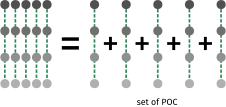
\includegraphics[width=0.5\textwidth]{decomposition.pdf}
% 	\caption{Because of the periodicity of the potential, the problem splits into a sum of particle on a circle (POC) problems, each formed by a specific crystal momentum and other momentum states that are related to it by a reciprocal vector.}
% \end{figure}
% We have used \(x^\prime\) to symbolise the position variable conjugate to the new set of momenta \(\left\{ nG \right\} = -i\partial_{x^\prime}\) that span the restricted Hilbert space of \(\mathcal{H}(k)\). Also, \(\mathcal{V}(k)\) is the Fourier transform of the real space potential \(V(x)\).
%
% This decoupling of the full Hamiltonian \(\mathcal{H}\) into a block-diagonal form (each block indexed by the crystal momentum \(k\)) can be attributed to the discrete translation symmetry present in the problem and could have been anticipated very generally, as we now show. The Hamiltonian satisfies \(\left[\mathcal{H}, T(a)\right] = 0\), where \(T(x) = e^{i \hat p x}\) is the translation operator. By choosing a starting location \(x=0\), applying the translation operator cycles through the set of states \(\ket{x=na}; ~n=0,1,\ldots,N_\text{well}\); this set is closed under the application of \(T(a)\). It is easy enough to guess the eigenstates of \(T(a)\). Since the application of \(T(a)\) increases the position monotonically, the only way to create an eigenstate is to involve all states. With that in mind, the simplest ansatz is of the form \(\ket{\Phi}= \sum_n e^{-i\Phi n} \ket{an}\). Applying the translation operator on this state gives 
% \begin{equation}\begin{aligned}
% 	T(a)\ket{\Phi} = \sum_{n=0}^{N_\text{well}-2} e^{-i\Phi n} \ket{a(n+1)} + e^{-i\Phi\left(N_\text{well} - 1\right) } \ket{aN_\text{well}} = e^{i\Phi}\left[e^{-i\Phi N_\text{well}} \ket{aN_\text{well}} + \sum_{n=1}^{N_\text{well}-1} e^{-i\Phi n} \ket{an}\right] 
% \end{aligned}\end{equation}
% Since we have applied PBC on the system, we used \(\ket{aN_\text{well}}\) for \(\ket{0}\). If the values of \(\Phi\) are chosen to be some integer multiple of \(2\pi/N_\text{well}\), we would have \(e^{-i\Phi N_\text{well}} = 1\), and the entire state can be resummed into the form
% \begin{equation}\begin{aligned}
% 	T(a)\ket{\Phi} = e^{i\Phi}\ket{\Phi}
% \end{aligned}\end{equation}
% This shows that \(\ket{\Phi}\) is an eigenstate of the translation operator. Since the set of states has a dimension of \(N_\text{well}\), the number of eigenstates and the number of possible values of \(\Phi\) will also be \(N_\text{well}\). This fixes the eigenvalues to \(\Phi = 2\pi m/N_\text{well}, m=0,1,\ldots,N_\text{well}-1\). These will also be eigenstates of the Hamiltonian, because they are indexed by different values of \(\Phi\)  and the Hamiltonian cannot change \(\Phi\) (because it commutes with \(T\)). As will be shown later, the eigenvalues \(\Phi\) are actually related to the crystal momentum, through \(\Phi=ka\). The set of allowed values of \(\Phi\) form the first Brillouin zone.
%
% However, \(\ket{\Phi}\) as defined above is not the only eigenstate with eigenvalue \(e^{i\Phi}\). One can simply shift the starting location \(x=0\) by any distance smaller than \(a\), and repeat the entire procedure. The eigenstates hence obtained will have the same eigenvalues as above:
% \begin{gather}
% 	\ket{\Phi, \delta}= \sum_n e^{-i\Phi n} \ket{an+\delta},~ 0\leq \delta < a;\\
% 	T(a)\ket{\Phi, \delta} = \sum_{n=0}^{N_\text{well}-2} e^{-i\Phi n} \ket{a(n+1) + \delta} + e^{-i\Phi\left(N_\text{well} - 1\right) + \delta} \ket{aN_\text{well} + \delta} = e^{i\Phi}\ket{\Phi, \delta}
% \end{gather}
% The translation operator is therefore able to at most classify the complete set of states into \(N_\text{well}\) number of blocks, each labelled by a specific value of \(\Phi\). Each block has a large number of states \((N_\text{levs})\), and the Hamiltonian will general scatter these states into each other. The Hamiltonian for each of these blocks can be represented as \(\mathcal{H}(\Phi) = \mathcal{P}_\Phi \mathcal{H} \mathcal{P}_\Phi\) (where \(\mathcal{P}_\Phi\) projects onto the block of states with eigenvalue \(e^{i\Phi}\)), such that the total Hamiltonian can be represented as \(\mathcal{H} = \sum_{\Phi} \mathcal{H}(\Phi)\). Upon rescaling by \(2\pi/a\) and taking the limit of \(N_\text{well} \to \infty\), this is the same Hamiltonian decoupling relation as that obtained in eq.~\ref{hamiltonianDecoupling}.
%
%
% Since the spacing between two adjacent momentum is \(G\), the maximum value of \(x^\prime\) has to be \(2\pi/G = a\), with the ends identified with each other: \(\psi(x^\prime=0) = \psi(x^\prime=a)\). We can then define a dimensionless variable \(\theta = 2\pi x^\prime/a\) that goes from \(0\) to \(2\pi\), and is conjugate to the angular wave number \(Q = -i\partial_\theta\). This definition ensures \(\left[\theta,Q\right] = i\). For reasons that will become clear very soon, we will also define a dimensionless crystal momentum \(\Phi = ka\). With these modifications, the Hamiltonian takes the simpler form
% \begin{equation}\begin{aligned}
% 	\mathcal{H}(k) &= \int_0^{2\pi}\mathrm{d\theta}~c^\dagger(\theta) \left[\frac{\hbar^2}{2ma^2}\left(\hat Q + \Phi/2\pi\right)^2 + U(\theta)\right]c(\theta)~.
% \end{aligned}\end{equation}
% By nothing  that we have the boundary condition \(\psi(\theta=0) = \psi(\theta=2\pi)\), we can recognise this Hamiltonian as that describing the dynamics of a particle moving on a circle (POC) with a potential \(U(\theta) = \frac{a}{2\pi}V(a\theta/2\pi)\), in the presence of an Aharonov-Bohm flux \(\Phi\). Note that \(U(\theta)\) has a period of \(2\pi\).
% \begin{figure}[htpb]
% 	\centering
% 	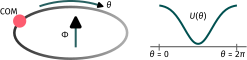
\includegraphics[width=0.7\textwidth]{POC.pdf}
% 	\caption{The full problem reduces to that of a particle on a circle, in the presence of potential with period \(2\pi\), and a flux \(\Phi\).}
% \end{figure}
%
% Even when reduced to the simpler POC, the problem cannot be simply integrated to obtain the eigenstates. This is because the complete Hamiltonian does not commute with either the position or the momentum operator; it contains quantum fluctuations that need to be resolved in order to obtain the ground state energy. One way of obtaining the energy is to calculate the propagator for transition from \(\theta=0\) to \(\theta=2\pi\), using the method of path integrals~\cite{rajaraman1982solitons,Weigert1994}. This is shown in Appendix~\ref{appendix_instanton}. We, however, will attack the problem using a renormalisation group method, called the unitary renormalisation group in order to track the emergence of the tight-binding metal in the limit when the effective amplitude of the single-particle periodic potential at low-energies has become much larger than the typical kinetic energy of the electron.
% \subsection*{URG analysis of the particle on a circle problem}
% A summary of the unitary RG method is provided in Appendix~\ref{appendix_urg}. For the purposes of studying the model under renormalisation group, we write the particle on a circle Hamiltonian in momentum\((Q-)\)space. For that, we introduce the Fourier modes 
% \begin{equation}\begin{aligned}
% 	c(\theta) = \frac{1}{\sqrt{2\pi}}\int dQ e^{iQ\theta}c(Q),~ \text{ and }~U(\theta) = \int dQ e^{iQ\theta}\mathcal{U}(Q)~,
% \end{aligned}\end{equation}
% so that the Hamiltonian becomes
% \begin{equation}\begin{aligned}
% \mathcal{H}(k) &= \int\mathrm{dQ}~\varepsilon\left(Q + \Phi/2\pi\right)\hat n(Q) + \int\mathrm{dQ_1}~\mathrm{dQ_2}~c^\dagger(Q_1)c(Q_2)\mathcal{U}\left( Q_1 - Q_2 \right) ~.
% \end{aligned}\end{equation}
% where we have defined the dispersion \(\varepsilon(Q) = \hbar^2 Q^2/(2ma^2)\).
% The second term involves scattering between momentum states \(Q_1\) and \(Q_2\). The quantum fluctuations that connect the low-energy states to the high-energy states can be integrated out using the URG method~\cite{AnirbanThesis}. This proceeds through a reduction in the momentum cutoff, ultimately leading to an IR theory. As the large momenta are integrated out, the potential term for scattering between the lower momenta undergo renormalisation.
% % \begin{figure}[htpb]
% % 	\centering
% % 	\includegraphics[width=0.4\textwidth]{URG_poc.pdf}
% % 	\caption{As the URG transformations are applied on the POC Hamiltonian, the connectivities with the high-energy momentum states (lighter gray) get integrated out, and these momentum states become integrals of motion. }
% % \end{figure}
% Let, at the \(l^\text{th}\) RG step, the momentum cutoff be \(Q_l\). At this step, fluctuations between all momentum states more energetic than \(Q_l\) have been integrated out. The RG equations for the renormalisation of the potential \(\mathcal{U}^{(l)}_{ij}\) that scatters any two lower momenta \(Q_i\) and \(Q_j\) \(\left( Q_i,Q_j < Q_l \right) \) is given by~\cite{AnirbanThesis}
% \begin{equation}\begin{aligned}
% 	\Delta \mathcal{U}_{ij}^{(l)}(\omega) = \frac{\mathcal{U}_{il}\mathcal{U}_{lj}}{\omega - \varepsilon(Q_l + \Phi/2\pi)}~,
% \end{aligned}\end{equation}
% where \(\omega\) is an energy scale that tracks the amount of quantum fluctuations present in the system, and is characteristic of the URG method. The dispersion also undergoes renormalisation::
% \begin{equation}\begin{aligned}
% 	\Delta \varepsilon^{(l)}(Q_i,\omega) = \frac{|\mathcal{U}_{il}|^2}{\omega - \varepsilon(Q_l + \Phi/2\pi)}~,
% \end{aligned}\end{equation}
%
% \subsection*{Effective description at low energies}
% \subsubsection*{Appearance of bands and band gaps}
% As the URG proceeds, the quantum fluctuations between the momentum states are resolved, leading to a simpler theory for the IR. We focus on the final two states \(\ket{Q_0 + \Phi/2\pi}, \ket{Q_1 + \Phi/2\pi}\), for \(\Phi=0\) (Brillouin zone edge). The Hamiltonian for their dynamics, just prior to the decoupling of \(Q_j\), is
% \begin{equation}\begin{aligned}
% 	H_{01}^* = \varepsilon^*(Q_0)\ket{Q_0}\bra{Q_0} + \varepsilon^{*}(Q_1)\ket{Q_1}\bra{Q_1} + \left(\mathcal{U}_{01}^{*}\ket{Q_1}\bra{Q_0} + \text{h.c.}\right)\label{fixed_point_two}
% \end{aligned}\end{equation}
% Since both the states are at the edge of the band, we can assume \(\varepsilon^{*}(Q_0) \simeq \varepsilon^{*}(Q_1)\), in which case the problem becomes that of a symmetric double well with tunnelling. The eigenstates are \(\ket{Q_0} \pm \ket{Q_1}\), with energies \(\varepsilon^{*}(Q_0) \pm |\mathcal{U}_{01}^{*}|\). We can substitute this estimate of the energy eigenvalues into the RG equations in the form of the quantum fluctuation scale \(\omega\). At the last decoupling, the shifts in the kinetic energy are therefore
% \begin{equation}\begin{aligned}
% 	\Delta \varepsilon^{*}(Q_i,\omega^\pm) \simeq \frac{|\mathcal{U}^{*}_{01}|^2}{\varepsilon^{*}(Q_0) \pm |\mathcal{U}_{01}^{*}| - \varepsilon(Q_0)} = \pm |\mathcal{U}^{*}_{01}| = \pm |\mathcal{U}^{*}(G)|~,
% \end{aligned}\end{equation}
% where we used \(\mathcal{U}_{01} = \mathcal{U}\left(Q_1 - Q_0\right) = \mathcal{U}(G)\).
% The difference between the two shifts gives the energy difference between the two lowest states of the POC. In this way, the above RG equation shows the emergence of the single-particle band gap and the formation of the band insulator (if the chemical potential is placed within the gap). If we now reintroduce the flux degree of freedom, the lowest energy eigenstates of all the POCs can be combined to form a band of closely spaced energy levels \(\left\{\varepsilon^{*}(Q_0 + \Phi_j/2\pi)\right\}, \Phi=k_{0,j}a \) (see Fig.\ref{fig:URGSpectrum-pdf}). These levels are indexed by \(k_{0,j}\) with \(j\) ranging through the first Brillouin zone; \(k_{0,j}\) are the crystal momenta of the system.
%
% The second band of states is formed similarly by considering the first excited of the POCs:\(\left\{\varepsilon^{*}(Q_1 + \Phi_j/2\pi)\right\}, \Phi=k_{0,j}a\). The gap between the first and second band is set by the energy difference between the ground state and first excited state of the POC at \(\Phi=0\). This difference, and hence the gap, is equal to \(2|\mathcal{U}_{01}^{*}|\).
%
% \begin{figure}[htpb]
% 	\centering
% 	\includegraphics[width=0.6\textwidth]{URGSpectrum.pdf}
% 	\caption{Spectral flow transformations on the POC by tuning the flux $\Phi$ generates the full band of delocalised single-particle electronic states whose crystal momenta correpond to 
% $\hbar\Phi/a$.}
% 	\label{fig:URGSpectrum-pdf}
% \end{figure}
%
% \subsubsection*{Dispersion relation of the lowest band}\label{disper}
% In order to derive the dispersion for the lowest band, we note that the final fixed point Hamiltonian (obtained upon decoupling all higher momentum states) is described by the single momentum state \(\ket{Q_0}\). In terms of real space hopping, this means that all short wavelength processes have been removed, and the only process that remains is the longest hopping, that from \(0\) to \(2\pi\). The fixed point Hamiltonian can be written in terms of this process:
% \begin{equation}\begin{aligned}
% 	\varepsilon^{*}(Q_0) \ket{Q_0}\bra{Q_0} = \frac{1}{2}\varepsilon^{*}(2\pi)\left( \ket{\theta=0} +  \ket{\theta=2\pi}\right) \left( \bra{\theta=0} +  \bra{\theta=2\pi}\right) = \frac{1}{2}\varepsilon^{*}(2\pi)\left( \hat n(0) + \hat n(2\pi) \right) \\
% 	+ \frac{1}{2}\varepsilon^{*}(2\pi)\left(c^\dagger(0)c(2\pi) + \text{h.c.}\right) 
% \end{aligned}\end{equation}
% We now recall that we had mapped the spatial point \(x=0\left(x=a\right)\) to the angular point \(\theta=0 \left(\theta=2\pi\right)\) point. We now transform back to spatial coordinates to get
% \begin{equation}\begin{aligned}
% \frac{1}{2}\varepsilon^{*}(2\pi)\left( \hat n(0) + \hat n(a) \right) + \frac{1}{2}\varepsilon^{*}(a)\left(c^\dagger(0)c(a) + \text{h.c.}\right)~.
% \end{aligned}\end{equation}
% This is computed for a specific value \(\Phi=0\) for the flux (or the crystal momentum). The POC corresponding to a particular flux is built from the states within a particular well. Changing the flux is then equivalent to studying the POC corresponding to the states within a different well. What this means is that tuning the flux by one interval amounts to translating the fixed point Hamiltonian by one period \(a\) of the potential. Adding the contributions from all the values of the flux leads to the following tight-binding Hamiltonian:
% \begin{equation}\begin{aligned}
% H_{TB}=	\varepsilon^{*}(2\pi)\sum_{j=0}^{N_\text{well}-1}\hat n(ja) + \frac{1}{2}\varepsilon^{*}(a)\sum_{j=0}^{N_\text{well}-1}\left(c^\dagger(ja)c((j+1)a) + \text{h.c.}\right)~,
% \end{aligned}\label{TB}\end{equation}
% where the first term corresponds to a constant chemical potential applied to the tight-binding metal in one dimension with a single-particle dispersion $\varepsilon (k) = -\varepsilon^{*}(a) \cos(ka)$ where $k$ corresponds to the set of crystal momenta $k\in\left[-\frac{\pi}{a},\frac{\pi}{a}\right]$. The exercise, therefore, shows the emergence of nearest-neighbour hopping in the lowest band by starting from a more microscopic model of a particle in a periodic potential. (An alternate derivation of the tight-binding metal has also been shown from path-integral methods in Appendix \ref{appendix_instanton}).
%
% \section{Alternative Approach Towards The URG: Starting from Anderson's Poor Man's Scaling Approach}
% \subsection*{Recasting Poor Man's scaling as a block-diagonalisation algorithm}
% We first describe the formalism of the poor man's scaling (PMS) method, first formulated by Anderson \cite{anderson1970}. The problem is defined as
% \begin{equation}\begin{aligned}
% 	\label{problem}
% \mathcal{H}\ket{\Psi} = E\ket{\Psi}
% \end{aligned}\end{equation}
% \(\mathcal{H}\) is the total Hamiltonian and \(\ket{\Psi}\) and \(E\) are the exact eigenstate and eigenvalue of \(\mathcal{H}\). We imagine a separation of the total Hilbert space into two set of states, and we call these two states \(\ket{0}\) and \(\ket{1}\). This separation depends on which scattering term we want to kill by this transformation. For example, in the URG, we typically select a particular electron \(q\beta\) and then kill the  scattering terms that change the number of this state. In that case, \(\ket{0}\) will refer to the set of states \(\left\{\ket{\hat n_{q\beta}=0}\otimes\ket{\phi_0}\right\}\) and \(\ket{1}\) will refer to the set of states \(\left\{\ket{\hat n_{q\beta}=1}\otimes\ket{\phi_1}\right\}\). \(\ket{\phi_{0,1}}\) refer to the states of all the other electrons. As another example, if we wanted to separate the charge-Kondo and the spin-Kondo from the SIAM, we would want to kill the terms that scatter between the spin-full subspace \(\hat n_d=1\) to the spin-less subspace \(\hat{n_d}=0,2\). These two will then be the \(\ket{0}\) and \(\ket{1}\) sets. 
%
% Keeping this separation in mind, the exact eigenstate \(\ket{\Psi}\) can be split as 
% \begin{equation}\begin{aligned}
% \ket{\Psi} = \sum_i \ket{\phi_0^i} + \sum \ket{\phi_1^i}
% \end{aligned}\end{equation}
% The Hamiltonian can also be split as 
% \begin{equation}\begin{aligned}
% \mathcal{H} = H_0 + V_+ + V_-
% \end{aligned}\end{equation}
% \(H_0\) does not scatter between \(\left\{\ket{0}\right\}\) and \(\left\{\ket{1}\right\}\). It contains the diagonal parts as well as scatterings inside the subspaces. \(V_\pm\) scatter between the subspaces:
% \begin{equation}\begin{aligned}
% V_+ \left\{\ket{0}\right\} \mapsto \left\{\ket{1}\right\},&& V_+ \ket{1} \to 0\\
% V_- \left\{\ket{1}\right\} \mapsto \left\{\ket{0}\right\},&& V_- \ket{0} \to 0
% \end{aligned}\end{equation}
% The Schrodinger equation can thus be split into
% \begin{equation}\begin{aligned}
% H_0 \sum_i \ket{\phi^i_0} + V_-\sum_i \ket{\phi^i_1} &= E \sum_i \ket{\phi^i_0}\\
% H_0 \sum_i \ket{\phi^i_1} + V_+\sum_i \ket{\phi^i_0} &= E \sum_i \ket{\phi^i_1}\\
% \end{aligned}\end{equation}
% Eliminating \(\sum_i \ket{\phi^i_1}\) gives
% \begin{equation}\begin{aligned}
% H_0 \sum_i \ket{\phi^i_0} + V_-\frac{1}{E_1 - H_0}V_+\sum_i \ket{\phi^i_0} &= E \sum_i \ket{\phi^i_0}\\
% \end{aligned}\end{equation}
% The effective Hamiltonian in this subspace is therefore
% \begin{equation}\begin{aligned}
% 	\tilde{\mathcal{H}}_0 = H_0 + V_-\frac{1}{E - H_0}V_+
% \end{aligned}\end{equation}
% Similarly, eliminating \(\sum_i \ket{\phi^i_0}\) gives the effective Hamiltonian in the other subspace,
% \begin{equation}\begin{aligned}
% 	\tilde{\mathcal{H}}_1 = H_0 + V_+\frac{1}{E - H_0}V_-
% \end{aligned}\end{equation}
% The total effective Hamiltonian that does not scatter between the two subspaces is
% \begin{equation}\begin{aligned}
% 	\tilde{\mathcal{H}}(E) = H_0 + \underbrace{V_-\frac{1}{E - H_0}V_+ +  V_+\frac{1}{E - H_0}V_-}_\text{renormalization}
% \end{aligned}\end{equation}
% This is of course a function of whatever exact energy eigenvalue we chose, \(E\). Different choices will give different effective Hamiltonians. The renormalization will now be written in terms of the matrix elements. Since the entire \(\mathcal{H}_X\) must be Hermitian, we must have \(V_- = V_+^\dagger \equiv V\).
% \begin{equation}\begin{aligned}
% \Delta \mathcal{H}(E) = V\frac{1}{E - H_0}V^\dagger +  V^\dagger\frac{1}{E - H_0}V
% \end{aligned}\end{equation}
% Now take the first term and insert complete bases on both sides of \(V\) and \(V^\dagger\).
% \begin{equation}\begin{aligned}
% V\frac{1}{E - H_0}V^\dagger &= \sum_{ijk}\ket{\phi_0^i}\bra{\phi_0^i}V\ket{\phi_1^j}\bra{\phi_1^j}\frac{1}{E - H_0}\ket{\phi_1^j}\bra{\phi_1^j}V^\dagger\ket{\phi_0^k}\bra{\phi_0^k} \\
% 							&= \sum_{ijk}\ket{\phi_0^i}V_{ij}\bra{\phi_1^j}\frac{1}{E - H_0}\ket{\phi_1^j}V^\dagger_{kj}\bra{\phi_0^k}~,
% \end{aligned}\end{equation}
% where we defined \(\bra{\phi_0^i}V\ket{\phi_1^j} = V_{ij}\). We now approximate \(H_0\) by keeping just the diagonal part, and allowing the balance to redefine \(E\) into \(\omega\). Then, \(\left(E - H_0\right) \ket{\phi_{0,1}^j} \equiv \left(\omega_{0,1} - E_{0,1}^j\right) \ket{\phi_{0,1}^j}\). That gives
% \begin{equation}\begin{aligned}
% \label{pms_dropV}
% V\frac{1}{E - H_0}V^\dagger &= \sum_{ijk}\ket{\phi_0^i}\bra{\phi_0^k}\frac{V_{ij}V^\dagger_{kj}}{\omega_1 - E^j_1}
% \end{aligned}\end{equation}
% The second term similarly gives
% \begin{equation}\begin{aligned}
% V^\dagger\frac{1}{E - H_0}V = \sum_{ijk}\ket{\phi_1^i}\bra{\phi_1^k}\frac{V^\dagger_{ji}V_{jk}}{\omega_0 - E^j_0}
% \end{aligned}\end{equation}
% The total renormalization becomes
% \begin{equation}\begin{aligned}
% 	\Delta \mathcal{H}(E) = \sum_{ijk}\left(\frac{1}{\omega_1 - E^j_1}\ket{\phi_0^i}\bra{\phi_0^k}V_{ij}V^\dagger_{kj} + \frac{1}{\omega_0 - E^j_0}\ket{\phi_1^i}\bra{\phi_1^k}V^\dagger_{ji}V_{jk}\right)
% \end{aligned}\end{equation}
% This is a general expression that would work irrespective of whether you are decoupling multiple electrons or a single electron. However, the \(\omega\) are unknown and we need some prescription for replacing them. Since the \(E\) is the eigenstate of the initial state on which the scattering terms act, it makes sense to replace them with the initial state energy.
% \begin{equation}\begin{aligned}
% 	\Delta \mathcal{H}(E) = \sum_{ijk}\left(\frac{1}{E_0^k - E^j_1}\ket{\phi_0^i}\bra{\phi_0^k}V_{ij}V^\dagger_{kj} + \frac{1}{E_1^k - E^j_0}\ket{\phi_1^i}\bra{\phi_1^k}V^\dagger_{ji}V_{jk}\right)
% \end{aligned}\end{equation}
% However, closer inspection reveals that this choice makes the renormalization non-Hermitian. So the correct choice is to keep both the initial and final energies.
% \begin{equation}\begin{aligned}
% 	\Delta \mathcal{H} =& \frac{1}{2}\sum_{ijk}\frac{1}{\omega_1 - E^j_1}\left(\ket{\phi_0^i}\bra{\phi_0^k}V_{ij}V^\dagger_{kj} + \ket{\phi_0^k}\bra{\phi_0^i}V_{kj}V^\dagger_{ij}\right)\\
% 						&+\frac{1}{2}\sum_{ijk}\frac{1}{\omega_0 - E^j_0}\left(\ket{\phi_1^i}\bra{\phi_1^k}V^\dagger_{ji}V_{jk} + \ket{\phi_1^k}\bra{\phi_1^i}V^\dagger_{jk}V_{ji}\right)\\
% 	=& \frac{1}{2}\sum_{ijk}\left(\frac{1}{E_0^k - E^j_1}\ket{\phi_0^i}\bra{\phi_0^k}V_{ij}V^\dagger_{kj} + \frac{1}{E_0^k - E^j_1}\ket{\phi_0^k}\bra{\phi_0^i}V_{kj}V^\dagger_{ij}\right) \\
% 	 &+\frac{1}{2}\sum_{ijk}\left(\frac{1}{E_1^k - E^j_0}\ket{\phi_1^i}\bra{\phi_1^k}V^\dagger_{ji}V_{jk} + \frac{1}{E_1^k - E^j_0}\ket{\phi_1^k}\bra{\phi_1^i}V^\dagger_{jk}V_{ji}\right)
% \end{aligned}\end{equation}
% Therefore,
% \begin{equation}\begin{aligned}
% 	\label{pmsren}
% 	\Delta \mathcal{H} &= \frac{1}{2}\sum_{ijk}\left(\frac{1}{E_0^k - E^j_1} + \frac{1}{E_0^i - E^j_1}\right)\ket{\phi_0^i}\bra{\phi_0^k}V_{ij}V^\dagger_{kj} +\frac{1}{2}\sum_{ijk}\left(\frac{1}{E_1^k - E^j_0}+ \frac{1}{E_1^i - E^j_0}\right)\ket{\phi_1^i}\bra{\phi_1^k}V^\dagger_{ji}V_{jk}\\
% \end{aligned}\end{equation}
% In summary, the prescription of replacing all \(\omega\) with the initial state energy will be correct only if the initial and final states are the same. This happens when we are decoupling a single-electron state - then the total renormalization is of the form \(c^\dagger T^\dagger c\) such that we start from an initial state, scatter to an intermediate state and then go back to the initial state so that the final state is the same as the initial state. However, if we are using PMS to decouple states in one-shot, each subspace will have multiple states and there might be terms where we do not end up at the initial state we started with. Then the correct prescription would be to use the mean of the initial and final state denominators.
%
% One might wonder how we can generate higher order terms in this method. Eq.~\ref{pmsren}, as it stands, has only \(\mathcal{O}(V^2)\) terms. The higher order terms were actually dropped when we replaced \(H_0\) with its diagonal part in eq.~\ref{pms_dropV}. To see the higher order term, we do not drop the off-diagonal part in the denominator, but split the total \(H_0\) into a diagonal and an off-diagonal part: \(H_0 = H_d + X\). Note that \(X\) is off-diagonal in the subspace of the states that have not been decoupled yet but will be decoupled later. They represent scattering between the lower energy states. \(X\) is still diagonal with respect to the states that we \text{are} decoupling presently. The total effective Hamiltonian becomes
% \begin{equation}\begin{aligned}
% 	\tilde{\mathcal{H}}(E) = H_0 + V\frac{1}{G_0(E)^{-1} - X}V^\dagger +  V^\dagger\frac{1}{G_0(E)^{-1} - X}V
% \end{aligned}\end{equation}
% where \(G_0(E)^{-1} = E - H_d\) is the inverse of the non-interacting Greens function. To allow computation, we can expand the denominator in powers of \(XG_0(E)^{-1}\):
% \begin{equation}\begin{aligned}
% 	\label{pms_third}
% 	\Delta H \equiv \tilde{\mathcal{H}}(E) - H_0 =& VG_0(E)\left[1 + XG_0(E) + XG_0(E)XG_0(E) + ...\right] V^\dagger +  V^\dagger\frac{1}{G_0(E)^{-1} - X}V\\
% 	=& \underbrace{V G_0(E) V^\dagger + V^\dagger G_0(E) V}_\text{two vertex or one loop correction} + \underbrace{VG_0(E)XG_0(E)V^\dagger + V^\dagger G_0(E)XG_0(E)V}_\text{three vertex or two loop correction} \\
% 			       &+ \text{higher loop corrections}
% \end{aligned}\end{equation}
%
% \subsection*{PMS in the language of the URG - obtaining the \(\eta\) operators}
% To make a better connection with URG, we next show how the PMS formalism works out for a single-electron decoupling. The corresponding problem can be phrased in the following manner. We want to decouple one electron at momentum \(q\) from the full Hamiltonian. We can split the exact wavefunction as
% \begin{equation}\begin{aligned}
% 	\label{wf}
% \ket{\Psi} = \ket{\Psi_0} + \ket{\Psi_1}
% \end{aligned}\end{equation}
% where \(\ket{\Psi_0} = \left(1 - \hat n_{q}\right)\ket{\Psi^N}\) is that part of the wavefunction where the state \(q\) is occupied. \(\ket{\Psi^N_1} = \hat n_q \ket{\Psi}\) is that part of the wavefunction where the state \(q\) is occupied. We can also split the Hamiltonian as
% \begin{equation}\begin{aligned}
% 	\label{hami}
% \mathcal{H} = \mathcal{H}^d + V_0 + V_+ + V_-
% \end{aligned}\end{equation}
% \(\mathcal{H}^d\) is the diagonal part; it has the purely energy terms as well as self-energies that may arise from the diagonal parts of interactions; \(V_0\) is the purely off-diagonal term that does not change \(\hat n_q\); it is the scattering \textit{inside} the low energy subspace. \(V_+\) and \(V_-\) are the purely off-diagonal terms that \textit{do} change \(\hat n_q\); \(V_+\) takes you from \(\hat n_q = 0\) to \(\hat n_q = 1\) and \(V_-\) does the opposite.
%
% Substituting eqs.~\ref{hami} and \ref{wf} in eq.~\ref{problem} gives
% \begin{equation}\begin{aligned}
% 	\left(\mathcal{H}^d + V_0 + V_+ + V_-\right)\left(\ket{\Psi_0} + \ket{\Psi_1}\right) = E\left(\ket{\Psi_0} + \ket{\Psi_1}\right)
% \end{aligned}\end{equation}
% Gathering the kets with \(\hat n_q = 0,1\) gives
% \begin{equation}\begin{aligned}
% 	\left(\mathcal{H}^d_0 + V_0\right)\ket{\Psi_0} + V_- \ket{\Psi_1} = E\ket{\Psi_0}\\
% 	\left(\mathcal{H}^d_1 + V_0\right)\ket{\Psi_1} + V_+\ket{\Psi_0} = E\ket{\Psi_1}
% \end{aligned}\end{equation}
% The second equation can be written as
% \begin{equation}\begin{aligned}
% \ket{\Psi_1} = \eta^\dagger \ket{\Psi_0}
% \end{aligned}\end{equation}
% where
% \begin{equation}\begin{aligned}
% 	\left(\eta^\dagger\right)_\text{PMS} = \frac{1}{E - \mathcal{H}^d_1 - V_0}V_+
% \end{aligned}\end{equation}
% Substituting this in the first equation gives
% \begin{equation}\begin{aligned}
% 	\label{reneq}
% 	\left(\mathcal{H}^d_0 + V_0 + V_- \eta^\dagger\right)\ket{\Psi_0} = E\ket{\Psi_0}
% \end{aligned}\end{equation}
% This new Hamiltonian,
% \begin{equation}\begin{aligned}
% 	\tilde{\mathcal{H}}_0 = \mathcal{H}^d_0 + V_0 + V_- \eta^\dagger
% \end{aligned}\end{equation}
% has the high energy mode removed; the scattering terms start from the low energy subspace and end at the low energy subspace as well. The renormalization in the low energy subspace scatterings  is
% \begin{equation}\begin{aligned}
% 	\label{deltaV}
% \Delta V_0 = V_- \eta^\dagger
% \end{aligned}\end{equation}
% If we eliminate \(\ket{\Psi_0}\) instead of \(\ket{\Psi_1}\), we get the renormalized equation in the high energy subspace:
% \begin{equation}\begin{aligned}
% \ket{\Psi_0} = \eta \ket{\Psi_1}
% \end{aligned}\end{equation}
% where
% \begin{equation}\begin{aligned}
% 	\left(\eta\right)_\text{PMS} = \frac{1}{E - \mathcal{H}^d_0 - V_0}V_-
% \end{aligned}\end{equation}
% ,so
% \begin{equation}\begin{aligned}
% 	\left(\mathcal{H}^d_1 + V_0 + V_+ \eta\right)\ket{\Psi_1} = E\ket{\Psi_1}
% \end{aligned}\end{equation}
% The renormalized Hamiltonian in the high energy subspace is thus
% \begin{equation}\begin{aligned}
% 	\tilde{\mathcal{H}}_1 = \mathcal{H}^d_1 + V_0 + V_+ \eta
% \end{aligned}\end{equation}
% If we want to keep both the high energy and low energy parts of the Hamiltonian, the new Hamiltonian is
% \begin{equation}\begin{aligned}
% 	\label{transham}
% 	\tilde{\mathcal{H}} &= \tilde{\mathcal{H}}_1 \hat n + \tilde{\mathcal{H}}_0 \left(1 - \hat n\right)\\
% &= \mathcal{H}^d_0 + \mathcal{H}^d_1 + V_0 + V_+ \eta + V_- \eta^\dagger
% \end{aligned}\end{equation}
% The total renormalization is
% \begin{equation}\begin{aligned}
% 	\left(\Delta \mathcal{H}\right)_\text{PMS} = V_+ \left(\eta\right)_\text{PMS} + V_- \left(\eta^\dagger\right)_\text{PMS}
% \end{aligned}\end{equation}
% It can be shown that if we define a unitary operator \(U = 1 - \eta + \eta^\dagger\), the transformed Hamiltonian \(U \mathcal{H} U^\dagger\) is the same as eq.~\ref{transham}. This, along with the properties of \(\eta\), have been shown in section \ref{urgform}. The important feature of eq.~\ref{transham} is that there is no term in the transformed Hamiltonian which scatters between \(\ket{\Psi_0}\) and \(\ket{\Psi_0}\)- the two subspaces have been truly decoupled.
% \begin{equation}\begin{aligned}
% 	\left[U \mathcal{H} U^\dagger, n_q\right] = 0
% \end{aligned}\end{equation}
% We can write down the renormalized Schrodinger equation in the low energy subspace, from eq.~\ref{reneq},
% \begin{equation}\begin{aligned}
% 	\tilde{\mathcal{H}}_0 \ket{\Psi_0} = E\ket{\Psi_0}
% \end{aligned}\end{equation}
% and again repeat the entire process. \(\tilde{\mathcal{H}}_0\) now takes the place of \(\mathcal{H}\) and \(\ket{\Psi_0}\) takes the place of \(\ket{\Psi}\) in eq.~\ref{problem}.
%
% The expression for URG is obtained in an almost identical way. The only difference is that instead of starting with the exact eigenpair (\(E,\ket{\Psi}\)), we start with a more general pair (\(\tilde{\mathcal{H}}, \ket{\Phi}\)) where \(\ket{\Phi}\) is not necessarily an exact eigenstate of \(\mathcal{H}\). It is defined by \(\mathcal{H}^\prime\), which is in turn defined as \(\hat n_q \mathcal{H}^\prime\left(1 - \hat n_q\right) = 0\). \(\ket{\Phi}\) is then defined by
% \begin{equation}\begin{aligned}
% \mathcal{H}\ket{\Phi} = \mathcal{H}^\prime \ket{\Phi}
% \end{aligned}\end{equation}
% This definition of \(\mathcal{H}^\prime\) is the very minimum that we must have in order to fulfill our goal (decouple \(q\)). 
%
% The operators \(\eta\) and its conjugate change accordingly:
% \begin{equation}\begin{aligned}
% 	\left(\eta\right)_\text{URG} &= \frac{1}{\tilde{\mathcal{H}} - \mathcal{H}^d_0 - V_0}V_-\\
%      &= \frac{1}{\hat \omega - \mathcal{H}^d_0}V_-\\
% \end{aligned}\end{equation}
% where \(\hat \omega \equiv \mathcal{H}^\prime - V_0\) now embodies the quantum fluctuations inherent in the Hamiltonian through the scattering term \(V_0\). Similarly,
% \begin{equation}\begin{aligned}
% 	\left(\eta^\dagger\right)_\text{URG} &= \frac{1}{\hat \omega - \mathcal{H}^d_1}V_+\\
% \end{aligned}\end{equation}
% The renormalization is again
% \begin{equation}\begin{aligned}
% 	\left(\Delta \mathcal{H}\right)_\text{URG} = V_+\left(\eta\right)_\text{URG} + V_-\left(\eta^\dagger\right)_\text{URG}
% \end{aligned}\end{equation}
% This again allows us to write down a unitary operator that decouples the entangled state:
% \begin{equation}\begin{aligned}
% 	U =  1 - \eta + \eta^\dagger, \left[\hat n_q, U \mathcal{H} U^\dagger\right] = 0
% \end{aligned}\end{equation}
% where \(\tilde{\mathcal{H}} = U^\dagger \mathcal{H} U\). We can now write down a new problem in this decoupled space with the rotated items and attempt to decouple another electron \(q^\prime\). We will again choose some general eigenpair (\(\mathcal{H}^\prime,\ket{\Phi}\)) such that \(\tilde{\mathcal{H}}\ket{\Phi} = \mathcal{H}^{\prime}\ket{\Phi}\) and \(\left[\mathcal{H}^{\prime},\hat n_{q^\prime}\right]=0\).
%
% Summarizing, the general Hamiltonian is not diagonal in the Fock space basis.
% URG, in order to proceed, selects one non-Fock basis of states \(\ket{\Phi}\) such that \(q\) is decoupled in that Hamiltonian.
% Since there can be lots of such basis, there is a freedom in this choice.
% With this basis in mind, URG then finds a unitary operator which when operated on the Hamiltonian takes us to the form in which it is diagonal in the Fock space basis.
% Note that this form is a function of the chosen \(\ket{\Phi}\).
% We then select the second degree of freedom and repeat the process.
% What PMS does is, it exploits the freedom of choice and selects the exact eigenstate \(\ket{\Psi}\) of the Hamiltonian as the non-Fock basis \(\ket{\Phi}\).
% Doing that returns a rotated Hamiltonian which is diagonal in \(q\), and is a function of the chosen state, same as URG. The conclusion is that depending on which state we choose as our diagonal non-Fock basis, URG and PMS will cause flows along different lines in general.
%
% As the couplings flow, \(V_0\) will also flow, leading to a flow of \(\hat\omega\). Just at the fixed point, the denominator of URG vanishes, giving the equation
% \begin{equation}\begin{aligned}
% 	\left(\hat\omega - \mathcal{H}_1^d\right)V_+\ket{\Psi_0} \text{ or } \left(\hat\omega - \mathcal{H}_1^d\right)V_-\ket{\Psi_1}
% \end{aligned}\end{equation}
% This means that one of the eigenvalues of \(\hat\omega\) matches with the eigenvalue of the diagonal part \(\mathcal{H}^d\), either in the occupied sector (\(\mathcal{H}^d_1\)) or unoccupied sector (\(\mathcal{H}^d_1\)). Since the eigenvalues are unchanged during the unitary renormalization, this implies that \(\omega\) takes up one of the eigenvalues of the whole Hamiltonian \(\mathcal{H}\). This will correspond to the fixed point obtained from PMS if we had started PMS with that eigenvalue.
%
% In short, while the PMS flow is parametrised by one of the exact energy eigenvalues \(E\), the URG flow is parametrised by a non-trivial operator \(\hat \omega\) which incorporates both a diagonal part and an off-diagonal part and itself flows under the URG. At the fixed point, the off-diagonal part cancels out and the \(\hat\omega\) finally flows to one of the energy eigenvalues and the URG fixed point matches with one of the PMS fixed points.
% \begin{figure}
% \centering
% \includegraphics[width=0.6\textwidth]{pms_vs_urg.png}
% \caption{Flows of PMS(green) and URG(blue)}
% \end{figure}
% \begin{itemize}
% \item The \textit{only} difference in the formalism of PMS and URG is that while PMS uses the exact energy eigenvalue \(E\) to parameterise the flow, URG uses a general intermediate decoupled Hamiltonian to do the same. Since the \(E\) is also, technically, an intermediate decoupled Hamiltonian (it is the final Hamiltonian), PMS can be seen as an URG but with a specific choice for the paramter.
% \item In practise, PMS replaces \(E-V_0\) with the diagonal part of the initial state at the current step of the RG. We are talking about the energy of the initial state, not the intermediate state. This is because, from eq.~\ref{problem}, \(E\) is the energy of the initial state on which \(V_\pm\) act. 
% \item The ideal solution would have been to substitute the exact energy and the total scattering term \(V\), but since we do not know \(E\) and keeping the \(V\) would make the thing untractable, we use our current best guess (renormalised diagonal part). As the RG flows, both \(E_j\) and \(V\) flow, such that at the fixed point, \(V\) becomes zero (scattering terms get removed) and \(E_j\) morphs into the exact \(E\). 
% \item In practise, URG replaces the \(\hat \omega\) with a guess for the final energy \(E\). This however ignores the renormalization of \(\hat \omega\). A better approach would be to replace it with \(E_j\), following PMS. That would act like the one-particle renormalization of \(\hat \omega\).
% \item PMS usually drops any diagonal component of the scattering from the denominator. For example, in the PMS of the Kondo model by Anderson \cite{anderson1970} or that of the anisotropic power law Kondo model by Chenge et.al \cite{tathagata_2015}, they do not keep the term \(J_z S_d^z s^z\) in the denominator although it is number(spin) conserving. Such terms are kept in the denominator of the URG though. It must be mentioned however that ref.~\cite{rukhsan_2017} \textit{does} bring a diagonal charge-charge interaction in the denominator in the PMS of the extended Anderson model.
% \end{itemize}
% \section{The Unitary RG as a non-perturbative Schrieffer-Wolff transformation}\label{sc_wl_t}
% \subsection*{Formalism}
% We have a general Hamiltonian
% \begin{equation}\begin{aligned}
% \mathcal{H} = \mathcal{H}_0 + \mathcal{H}_X
% \end{aligned}\end{equation}
% \(\mathcal{H}_0\) is diagonal w.r.t a particular degree of freedom. \(V\) is off-diagonal w.r.t that same degree of freedom. Let \(S\) be an \textit{anti-Hermitian} and \textit{off-diagonal} operator. \(U = e^S\) is then a unitary transformation.
% \begin{equation}\begin{aligned}
% 	U \mathcal{H} U^\dagger &= e^S \left(\mathcal{H}_0 + \mathcal{H}_X\right)e^{-S}\\
% 				&= \left(\cosh\left(S\right) + \sinh\left(S\right)\right)\left(\mathcal{H}_0 + \mathcal{H}_X\right)\left(\cosh\left(S\right) - \sinh\left(S\right)\right)\\
%          &= H_1 + H_2
% \end{aligned}\end{equation}
% where \(H_1\) is diagonal and \(H_2\) is off-diagonal.
% \begin{equation}\begin{aligned}
% 	H_1=\cosh\left(S\right) \mathcal{H}_0 \cosh\left(S\right) - \sinh\left(S\right) \mathcal{H}_0 \sinh\left(S\right) -\cosh\left(S\right) \mathcal{H}_X \sinh\left(S\right)\\
% 	+\sinh\left(S\right) \mathcal{H}_X \cosh\left(S\right)\\
% 	H_2 = - \cosh\left(S\right) \mathcal{H}_0 \sinh\left(S\right) + \sinh\left(S\right) \mathcal{H}_0 \cosh\left(S\right) +\cosh\left(S\right) \mathcal{H}_X \cosh\left(S\right)\\
% 	-\sinh\left(S\right) \mathcal{H}_X \sinh\left(S\right)
% \end{aligned}\end{equation}
% The decoupling condition is \(H_2=0\).
%
% For small \(S\), we have \(\sinh S \sim S\) and \(\cosh S \sim 1 + \frac{1}{2} S^2\). Therefore, the off-diagonal part, up to second order, is 
% \begin{equation}\begin{aligned}
% 	H_2 = -\mathcal{H}_0 S + S \mathcal{H}_0 + \mathcal{H}_X + O(S^3) = \left[S,\mathcal{H}_0\right] + \mathcal{H}_X
% \end{aligned}\end{equation}
% The second order decoupling condition is thus
% \begin{equation}\begin{aligned}
% 	\label{dec_cond}
% 	\left[S,\mathcal{H}_0\right] = -\mathcal{H}_X
% \end{aligned}\end{equation}
% The effective Hamiltonian is what remains, \(H_1\). That becomes, at second order,
% \begin{equation}\begin{aligned}
% 	H_1 &= \left(1 + \frac{1}{2} S^2\right) \mathcal{H}_0 \left(1 + \frac{1}{2} S^2\right) - S \mathcal{H}_0 S -\left(1 + \frac{1}{2} S^2\right) \mathcal{H}_X S + S \mathcal{H}_X \left(1 + \frac{1}{2} S^2\right)\\
%     &= \mathcal{H}_0 + \frac{1}{2} \left\{S^2, \mathcal{H}_0\right\} - S \mathcal{H}_0 S - \mathcal{H}_X S + S \mathcal{H}_X + O(S^3)\\
%     &= \mathcal{H}_0 + \frac{1}{2} S\left[S, \mathcal{H}_0\right] - \frac{1}{2} \left[S, \mathcal{H}_0\right]S  + \left[S,\mathcal{H}_X\right] + O(S^3)\\
%     &= \mathcal{H}_0 + \frac{1}{2} \left[S,\left[S, \mathcal{H}_0\right]\right] + \left[S,\mathcal{H}_X\right] + O(S^3)\\
%     &= \mathcal{H}_0 + \frac{1}{2} \left[S,-\mathcal{H}_X\right] + \left[S,\mathcal{H}_X\right] + O(S^3)\\
%     &= \mathcal{H}_0 + \frac{1}{2}\left[S,\mathcal{H}_X\right] + O(S^3)\\
% \end{aligned}\end{equation}
% Avoiding the perturbative route, we can take \(S = \frac{\pi}{4}\left(\eta^\dagger - \eta\right)\), where \(\eta\) and its conjugate are non-perturbative and Fermionic - they satisfy \(\eta^2 = {\eta^\dagger}^2 = 0\) and \(\left\{\eta,\eta^\dagger\right\}=1\). We can then write
% \begin{equation}\begin{aligned}
% 	e^S &= \exp\left\{\frac{\pi}{4}\left(\eta^\dagger - \eta\right)\right\} \\
% 	    &= 1 + \left(\eta^\dagger - \eta\right)\frac{\pi}{4} + \frac{1}{2!}\left(\eta^\dagger - \eta\right)^2\left(\frac{\pi}{4}\right)^2 + \frac{1}{3!}\left(\eta^\dagger - \eta\right)^3\left(\frac{\pi}{4}\right)^3 + ...\\
% 	    &= 1 + \left(\eta^\dagger - \eta\right)\frac{\pi}{4} - \frac{1}{2!}\left(\frac{\pi}{4}\right)^2 - \frac{1}{3!}\left(\eta^\dagger - \eta\right)\left(\frac{\pi}{4}\right)^3 + \frac{1}{4!}\left(\frac{\pi}{4}\right)^4 + ...\\
% 	    &= \cos \frac{\pi}{4} + \left(\eta^\dagger - \eta\right)\sin\frac{\pi}{4}\\
% 	    &= \frac{1}{\sqrt 2}\left(1 + \eta^\dagger - \eta\right)
% \end{aligned}\end{equation}
% There we used
% \begin{equation}\begin{aligned}
% 	\left(\eta^\dagger - \eta\right)^2 = {\eta^\dagger}^2 + \eta^2 - \left\{\eta^\dagger,\eta\right\} = -1 &&\left[\because\eta^2 = {\eta^\dagger}^2=0\right]
% \end{aligned}\end{equation}
% and hence
% \begin{equation}\begin{aligned}
% 	\left(\eta^\dagger - \eta\right)^3 = -1\left(\eta^\dagger - \eta\right)
% \end{aligned}\end{equation}
% and so on. This simplification allows us to write
% \begin{equation}\begin{aligned}
% 	\label{cossin}
% 	\cosh S = \frac{1}{2}\left[e^S + e^{-S}\right] = \frac{1}{2\sqrt 2}\left(1 + \eta^\dagger - \eta + 1 - \eta^\dagger + \eta\right) = \frac{1}{\sqrt 2}
% \end{aligned}\end{equation}
% and
% \begin{equation}\begin{aligned}
% 	\sinh S = \frac{1}{2}\left[e^S - e^{-S}\right] = \frac{1}{2\sqrt 2}\left(1 + \eta^\dagger - \eta - 1 + \eta^\dagger - \eta\right) = \frac{1}{\sqrt 2}\left(\eta^\dagger - \eta\right)
% \end{aligned}\end{equation}
% The off-diagonal part now becomes
% \begin{equation}\begin{aligned}
% 	H_2 = \frac{1}{2}\left(\mathcal{H}_X - \eta^\dagger \mathcal{H}_X \eta^\dagger - \eta \mathcal{H}_X \eta + \left[\eta^\dagger - \eta, \mathcal{H}_0\right]\right)
% \end{aligned}\end{equation}
% The vanishing of this quantity is now the decoupling condition, and is also given in eq 16 of ref.~\cite{anirbanurg1}.
%
% To look for a decoupling condition similar to eq.~\ref{dec_cond}, we can re-express the \(\cosh\) and \(\sinh\) in eq.~\ref{cossin} in terms of \(S\), by substituting \(\eta^\dagger - \eta = \frac{4}{\pi}S\):
% \begin{equation}\begin{aligned}
% \cosh S = \frac{1}{\sqrt 2},\text{ and } \sinh S = \frac{4}{\sqrt 2 \pi}S
% \end{aligned}\end{equation}
% That gives
% \begin{equation}\begin{aligned}
% 	H_2 = \frac{1}{2}\left(\frac{4}{\pi}\left[S,\mathcal{H}_0\right] + \mathcal{H}_X - \frac{16}{\pi^2}S \mathcal{H}_X S\right)
% \end{aligned}\end{equation}
% The decoupling condition becomes
% \begin{equation}\begin{aligned}
% 	\left[S,\mathcal{H}_0\right] = -\frac{\pi}{4}\mathcal{H}_X + \frac{4}{\pi}S \mathcal{H}_X S
% \end{aligned}\end{equation}
% This can be compared to the second order condition: \(\left[S,\mathcal{H}_0\right] = -\mathcal{H}_X\). We  can also write the effective Hamiltonian for this non-perturbative case.
% \begin{equation}\begin{aligned}
% 	U\mathcal{H} U^\dagger = H_1 = \frac{1}{2} \mathcal{H}_0 - \frac{4}{\pi^2}S\mathcal{H}_0 S  + \frac{2}{\pi}\left[S,\mathcal{H}_X\right]
% \end{aligned}\end{equation}
% The differences between the perturbative and non-perturbative ways are summarized in table \ref{comparison}.
% \begin{table}
% % \def\tabcolsep=10pt
% \centering
% \begin{tabular}{|c|c|c|}
%     \hline
%         &renormalization&decoupling condition\\
%     \hline
% 	SWT&\(\frac{1}{2} \left[S,\mathcal{H}_X\right]\)&\(\left[S,\mathcal{H}_0\right] = -\mathcal{H}_X\)\\
% 	URG&\(\frac{2}{\pi}\left[S,\mathcal{H}_X\right]\)&\(\left[S,\mathcal{H}_0\right] = -\frac{\pi}{4}\mathcal{H}_X + \frac{4}{\pi}S \mathcal{H}_X S\)\\
%     \hline
% \end{tabular}
%     \caption{Comparison of perturbative and non-perturbative canonical transformations}
%     \label{comparison}
% \end{table}
% There appear to be two differences between these decoupling conditions: (a)  a pre-factor of \(\frac{\pi}{4}\) for the first term on the right hand side, and (b) the altogether new second term on the right hand side. Both are outcomes of the non-perturbative nature of URG. This offers evidence that the physics captured by the effective Hamiltonian (and its associated low-energy many-particle Hilbert space) obtained from URG lies well beyond that obtained from SWT. Further, it shows that the SWT can only be justified as an expansion in a small parameter (say, $\frac{1}{U}$) in the Anderson impurity problem), followed by a truncation of the BCH expansion and a projection onto a particular low-energy subspace. The truncation and projection are adopted simultaneously, and appear to impose the limit of \(U = \infty\) by hand. The URG flow never attains such a limit, thus suggesting that there exists a lot of interesting physics that could potentially be lost in the SWT procedure. Further, the projection finally applied within SWT means that we can never recover what is thrown away. This is again not the case with URG.
% \subsection*{Obtaining renormalization via Schrieffer-Wolff transformation - Comparison with Poor Man's scaling and URG}
% Similar to the situation in Poor Man's scaling, one can visualize two set of states and let \(\mathcal{H}_X = V_+ + V_-\) be the scattering that connects them and hence the one we want to kill. Let \(S\) be of the form 
% \begin{equation}\begin{aligned}
% 	S = \sum_{ij}\left[s\ket{\phi_1^i}\bra{\phi_0^j} - s^\dagger\ket{\phi_0^j}\bra{\phi_1^i}\right]
% \end{aligned}\end{equation}
% This form is of course chosen to make \(S\) anti-Hermitian and off-diagonal. The part \(s\) can be determined from the decoupling condition:
% \begin{equation}\begin{aligned}
% 	-\mathcal{H}_X = \left[S, H_0\right] = S H_0 - H_0 S
% \end{aligned}\end{equation}
% Multiplying with \(\bra{\phi_0^a}\) and \(\ket{\phi_1^b}\) from the left and right respectively gives
% \begin{equation}\begin{aligned}
% -\bra{\phi_0^a}V + V^\dagger\ket{\phi_1^b} &= \bra{\phi_0^a}S H_0 - H_0 S\ket{\phi_1^b}\\
% \end{aligned}\end{equation}
% Since \(V^\dagger\) acts on \(\ket{0}\), it will not affect the LHS. Also, \(\bra{\phi_0^a}V\ket{\phi_1^b} = V_{ab}\). If we now consider only the diagonal part of \(H_0\), we can write \(H_0 (\ket{\phi_0^a},\ket{\phi_1^b}) = (E_{0,a}\ket{\phi_0^a},E_{1,b}\ket{\phi_1^b}))\). We then get
% \begin{equation}\begin{aligned}
% 	-V_{ab} &= \bra{\phi_0^a}\sum_i\left[S\ket{\phi_1^i}\bra{\phi_1^i} H_0 - H_0 \ket{\phi_0^i}\bra{\phi_0^i}S\right]\ket{\phi_1^b} = \sum_i\left[S_{ai}E_1^i \delta_{bi} - E^i_0 \delta_{ai}S_{ib}\right] = S_{ab}E_1^b  - E^a_0 S_{ab}\\
% \implies S_{ab} &= \frac{V_{ab}}{E_0^a - E_1^b}
% \end{aligned}\end{equation}
% where we defined \(\bra{\phi_0^x}S\ket{\phi_1^y} = S_{xy}\). The total generator is
% \begin{equation}\begin{aligned}
% 	\label{swtgen}
% 	S &= \sum_{ij}\left[S_{ij}\ket{\phi_0^i}\bra{\phi_1^j} - S_{ij}^\dagger\ket{\phi_1^j}\bra{\phi_0^i}\right]= \sum_{ij}\frac{1}{E_0^i - E_1^j}\left[V_{ij}\ket{\phi_0^i}\bra{\phi_1^j} - V^\dagger_{ij}\ket{\phi_1^j}\bra{\phi_0^i}\right]\\
% \end{aligned}\end{equation}
% The renormalization is thus
% \begin{equation}\begin{aligned}
% 	\Delta \mathcal{H} &= \frac{1}{2} \left[S,\mathcal{H}_X\right]\\
% 			   &= \frac{1}{2} \sum_{ij,kl}\left[\frac{1}{E_0^i - E_1^j}\left(V_{ij}\ket{\phi_0^i}\bra{\phi_1^j} - V^\dagger_{ij}\ket{\phi_1^j}\bra{\phi_0^i}\right), V_{kl} \ket{\phi_0^k}\bra{\phi_1^l}+ V^\dagger_{kl} \ket{\phi_1^l}\bra{\phi_0^k}\right]\\
%                   &= \frac{1}{2} \sum_{ij,kl}\left[\frac{1}{E_0^i - E_1^j}\left(V_{ij}V^\dagger_{kl}\ket{\phi_0^i}\bra{\phi_0^k}\delta_{jl} - V^\dagger_{ij}V_{kl}\ket{\phi_1^j}\bra{\phi_1^l}\delta_{ik}\right.\right.\\
%                   &\quad\left.\left.- V^\dagger_{kl}V_{ij}\ket{\phi_1^l}\bra{\phi_1^j}\delta_{ki} + V_{kl}V^\dagger_{ij}\ket{\phi_0^k}\bra{\phi_0^i}\delta_{lj}\right)\right]\\
%                   &= \frac{1}{2} \sum_{ijk}\left[\frac{1}{E_0^i - E_1^j}\left(V_{ij}V^\dagger_{kj}\ket{\phi_0^i}\bra{\phi_0^k} - V^\dagger_{ij}V_{ik}\ket{\phi_1^j}\bra{\phi_1^k}- V^\dagger_{ik}V_{ij}\ket{\phi_1^k}\bra{\phi_1^j} + V_{kj}V^\dagger_{ij}\ket{\phi_0^k}\bra{\phi_0^i}\right)\right]\\
% 		  &= \frac{1}{2} \sum_{ijk}\left[\left(\frac{1}{E_0^i - E_1^j} + \frac{1}{E_0^k - E_1^j}\right)V_{ij}V^\dagger_{kj}\ket{\phi_0^i}\bra{\phi_0^k} - \left(\frac{1}{E_0^i - E_1^j} + \frac{1}{E_0^i - E_1^k}\right)V^\dagger_{ij}V_{ik}\ket{\phi_1^j}\bra{\phi_1^k}\right]\\
% \end{aligned}\end{equation}
% This is the same as the PMS result eq.~\ref{pmsren}. It is easy to see that since this transformation is unitary, it has zero trace so as to preserve the trace of the Hamiltonian:
% \begin{equation}\begin{aligned}
% 	\text{Tr}\left[\mathcal{H}\right] &= \sum_{l}\left(\bra{\phi_0^l} + \bra{\phi_1^l}\right)\Delta \mathcal{H}\left(\ket{\phi_0^l} + \ket{\phi_1^l}\right) = \frac{1}{2} \sum_{jl}\frac{2}{E_0^l - E_1^j}V_{lj}V^\dagger_{lj} - \frac{1}{2} \sum_{ji}\frac{2}{E_0^i - E_1^l}V^\dagger_{il}V_{il} = 0
% \end{aligned}\end{equation}
%
% We can also make a comparison to the renormalization obtained from URG.
% \begin{equation}\begin{aligned}
% 	\Delta \mathcal{H} &= \frac{1}{2}\left[\eta^\dagger - \eta,\mathcal{H}\right]
% \end{aligned}\end{equation}
% where 
% \begin{equation}\begin{aligned}
% \eta &= \frac{1}{\omega - \mathcal{H}^d}\sum_{ij}V_{ij}\ket{\phi_0^i}\bra{\phi_1^j} = \sum_{ij}\frac{1}{\omega_1^j - E_0^i}V_{ij}\ket{\phi_0^i}\bra{\phi_1^j}\\
% \implies \eta^\dagger &= \sum_{ij}\frac{1}{\omega_1^j - E_0^i}V^\dagger_{ij}\ket{\phi_1^j}\bra{\phi_0^i}\\
% \implies \eta^\dagger - \eta &= \sum_{ij}\frac{1}{\omega_1^j - E_0^i}\left(V^\dagger_{ij}\ket{\phi_1^j}\bra{\phi_0^i} - V_{ij}\ket{\phi_0^i}\bra{\phi_1^j}\right)\\
% \end{aligned}\end{equation}
% This can be thought of as the generator for the unitary transformations of URG. Comparing with the generator \(S\) of eq.~\ref{swtgen}, the prescription to go from URG to SWT is to replace \(\omega_1^j \to E_1^j\). Doing a similar calculation gives
% \begin{equation}\begin{aligned}
% 	\Delta \mathcal{H}_{URG} = \frac{1}{2} \sum_{ijk}\left[\left(\frac{1}{E_0^i - \omega_1^j} + \frac{1}{E_0^k - \omega_1^j}\right)V_{ij}V^\dagger_{kj}\ket{\phi_0^i}\bra{\phi_0^k} - \left(\frac{1}{E_0^i - \omega_1^j} + \frac{1}{E_0^i - \omega_1^k}\right)V^\dagger_{ij}V_{ik}\ket{\phi_1^j}\bra{\phi_1^k}\right]\\
% \end{aligned}\end{equation}
%
% \section{A comparison of URG, SWT and PMS on the Anderson model}
% The SWT for the single-impurity Anderson model is briefly sketched below. In order to decouple a state \(q\beta\) from the SIAM (\(\epsilon_q > 0\)) , we take an ansatz \(S = (A + B\hat n_{d\overline\beta})(c^\dagger_{q\beta}c_{d\beta} - \text{h.c.})\). Plugging this into the decoupling condition gives
% \begin{equation}\begin{aligned}
% 	-\epsilon_q\left(A + B\hat n_{d\overline\beta}\right) + \epsilon_d\left(A + B\hat n_{d\overline\beta}\right) + U\left(A + B\right)\hat n_{d\overline\beta} = -V
% \end{aligned}\end{equation}
% which gives
% \begin{equation}\begin{aligned}
% 	S = V\left[\frac{1 - \hat n_{d\overline\beta}}{\epsilon_q - \epsilon_d} + \frac{\hat n_{d\overline\beta}}{\epsilon_q - \epsilon_d - U}\right] (c^\dagger_{q\beta}c_{d\beta} - \text{h.c.})
% \end{aligned}\end{equation}
% The remaining diagonal part constitutes the effective Hamiltonian.
% \begin{equation}\begin{aligned}
% 	U\mathcal{H} U^\dagger = H_1 &= \mathcal{H}_0 + \frac{1}{2} \left\{\mathcal{H}_0, S^2\right\} - S \mathcal{H}_0 S + \left[S,\mathcal{H}_X\right]\\
% 				     &=\mathcal{H}_0 + \frac{1}{2} \left[\left[\mathcal{H}_0, S\right],S\right] + \left[S,\mathcal{H}_X\right]\\
% 				     &=\mathcal{H}_0 + \frac{1}{2} \left[\mathcal{H}_X,S\right] + \left[S,\mathcal{H}_X\right]\\
% 				     &=\mathcal{H}_0 + \frac{1}{2} \left[S,\mathcal{H}_X\right]
% \end{aligned}\end{equation}
% For the SIAM (and noting that we are decoupling \(q\beta\)), the two parts are
% \begin{equation}\begin{aligned}
% 	\mathcal{H}_0 &= \sum_{k\sigma}\epsilon_k \hat n_{k\sigma} + \epsilon_d \hat n_d + U\hat n_{d\uparrow}\hat n_{d\downarrow} + \sum_{k\sigma \neq q\beta}\left(c^\dagger_{k\sigma}c_{d\sigma} + \text{h.c.}\right)\\
% \mathcal{H}_X &= c^\dagger_{q\beta}c_{d\beta} + \text{h.c.} 
% \end{aligned}\end{equation}
% The renormalization in the effective Hamiltonian from decoupling a high energy particle state is thus
% \begin{equation}\begin{aligned}
% 	\frac{1}{2} \left[S,\mathcal{H}_X\right]\bigg\vert_{\hat n_{q\beta}=0} &= |V|^2\left[\frac{1 - \hat n_{d\overline\beta}}{\epsilon_q - \epsilon_d} + \frac{\hat n_{d\overline\beta}}{\epsilon_q - \epsilon_d - U}\right]\left[\hat n_{q\beta}\left(1 - \hat n_{d\beta}\right) - \hat n_{d\beta}\left(1 - \hat n_{q\beta}\right)\right]\bigg\vert_{\hat n_{q\beta}=0}\\
% 									       &=-\hat n_{d\beta}|V|^2\left[\frac{1 - \hat n_{d\overline\beta}}{\epsilon_q - \epsilon_d} + \frac{\hat n_{d\overline\beta}}{\epsilon_q - \epsilon_d - U}\right]
% \end{aligned}\end{equation}
% In the last step, we put \(\hat n_{q\beta}=0\) because previously we assumed \(\epsilon_q>0\) and high energy virtual excitations above the Fermi surface must necessarily be vacant in the initial state (at \(T=0\)). We can obtain the renormalization from decoupling a high energy \textit{hole} state directly from this expression, just by choosing \(\hat n_{q\beta}=1\) and setting \(\epsilon_q \to -\epsilon_q\).
% \begin{equation}\begin{aligned}
% 	\frac{1}{2} \left[S,\mathcal{H}_X\right]\bigg\vert_{\hat n_{q\beta}=1} &=-\left(1 - \hat n_{d\beta}\right)|V|^2\left[\frac{1 - \hat n_{d\overline\beta}}{\epsilon_q + \epsilon_d} + \frac{\hat n_{d\overline\beta}}{\epsilon_q + \epsilon_d + U}\right]
% \end{aligned}\end{equation}
% These two results - the renormalization in the particle and hole sectors - is identical to the result obtained from PMS of the SIAM~\cite{haldane1978scaling,jefferson_1977}. The renormalizations in the various energy levels of the impurity can be read off now, after summing over all states in the interval we are decoupling.
% \begin{equation}\begin{aligned}
% \Delta E_2 &= -2\sum_{q}\frac{|V_q|^2}{\epsilon_q - \epsilon_d - U}\\
% \Delta E_1 &= -\sum_{q}\frac{|V_q|^2}{\epsilon_q - \epsilon_d} - \sum_{q}\frac{|V_q|^2}{\epsilon_q + \epsilon_d + U}\\
% \Delta E_0 &= -2\sum_{q}\frac{|V_q|^2}{\epsilon_q + \epsilon_d}\\
% \end{aligned}\end{equation}
% This can be compared with the URG result, eq.~\ref{urg-siam},
% \begin{equation}\begin{aligned}
% \Delta E_2 &= 2\sum_{q}\frac{|V_q|^2}{\omega - \frac{1}{2}\epsilon_q + \epsilon_d + U}\\
% \Delta E_1 &= \sum_{q}\frac{|V_q|^2}{\omega - \frac{1}{2}\epsilon_q - \epsilon_d - U} + \sum_{q}\frac{|V_q|^2}{\omega - \frac{1}{2}\epsilon_q + \epsilon_d}\\
% \Delta E_0 &= 2\sum_{q}\frac{|V_q|^2}{\omega - \frac{1}{2}\epsilon_q - \epsilon_d}\\
% \end{aligned}\end{equation}
% We can transform the URG result to the SWT result if we ignore the effect of the quantum fluctuations in \(\omega\) (arising from the presence of the off-diagonal term \(\mathcal{H}^i\)) and replace it with the renormalised diagonal value of \(-\frac{1}{2}\epsilon_q\). This means that SWT tracks the effect of the off-diagonal terms only in the numerator. Of course, all this assumes we are doing an iterative SWT instead of a one-shot SWT; the latter is the conventional way. A second difference is that URG has a Green's function like structure in the renormalization such that a fixed point is reached when the diagonal part \(\mathcal{H}^d\) matches one of the eigenvalues of \(\omega\) (see \ref{match}). SWT does not have such a fixed point structure.
%
% Another point to note is that decoupling a single electron does not generate all the charge-charge or spin-spin interactions that come out when one performs a one-shot SWT. This implies that such terms are a result of decoupling the non-local interactions of the impurity (it is talking to all the mobile electrons), and cannot be generated when we remove just the local interactions of the mobile electrons. Instead, if one performs a URG in which we non-perturbatively kill the 2-point vertices in the SIAM, such 4-point vertices are generated. This is shown in the next subsection.
% \section{Deriving the Kondo model from the Anderson model via a one-shot URG}\label{SWT from URG}
% Here we will show how we can obtain the spin-spin interaction of the Kondo model by performing a one-shot URG on the SIAM. This should justify that the action of performing an SWT is analogous to decoupling the whole band via URG. 
% There are three departures from the conventional way of doing URG (or PMS).
% \begin{itemize}
%     \item We will be severing the connections of the impurity with all the mobile electrons in one-shot, and not iteratively.
%     \item We will have to trivialize the quantum fluctuation operator \(\hat \omega\) by replacing it with the diagonal part of the initial state energy.
% \end{itemize}
% Since we are decoupling the whole band, the off-diagonal part that we want to remove is
% \begin{equation}\begin{aligned}
% 	\mathcal{H}^I = \sum_{k\sigma}\left[V_k c^\dagger_{k\sigma}c_{d\sigma}+\text{h.c.}\right]
% \end{aligned}\end{equation}
% The diagonal part is the rest of the Hamiltonian.
% \begin{equation}\begin{aligned}
% \mathcal{H}^d &= \sum_{k\sigma}\epsilon_k\hat n_{k\sigma} + \epsilon_d\hat n_d + U\hat n_{d\uparrow}\hat n_{d\downarrow} = \sum_{k\sigma}\epsilon_k\tau_{k\sigma} + \epsilon_d\hat n_d + U\hat n_{d\uparrow}\hat n_{d\downarrow}\\
% \end{aligned}\end{equation}
% Following eq.~\ref{renurg}, the renormalization is
% \begin{equation}\begin{aligned}
% 	\Delta \mathcal{H} = \frac{1}{2}\left[\eta^\dagger - \eta, \mathcal{H}_X\right]
% \end{aligned}\end{equation}
% The transition operator \(\eta\) is
% \begin{equation}\begin{aligned}
% 	\label{swturg}
% \eta &= \frac{1}{\omega - \mathcal{H}^d}\sum_{k\sigma}V^*_k c^\dagger_{d\sigma}c_{k\sigma}= \sum_{k\sigma}\frac{1}{\omega + \frac{1}{2}\epsilon_k - \epsilon_d - \left(\epsilon_d + U\right)\hat n_{d\overline\sigma}}V^*_k c^\dagger_{d\sigma}c_{k\sigma}\\
%      &= \sum_{k\sigma}\left[\frac{\hat n_{d\overline\sigma}}{\omega_1 + \frac{1}{2}\epsilon_k - 2\epsilon_d - U} + \frac{1 - \hat n_{d\overline\sigma}}{\omega_0 + \frac{1}{2}\epsilon_k - \epsilon_d}\right]V^*_k c^\dagger_{d\sigma}c_{k\sigma}= \sum_{k\sigma}\left[\frac{\hat n_{d\overline\sigma}}{E_k^1} + \frac{1 - \hat n_{d\overline\sigma}}{E_k^0}\right]V^*_k c^\dagger_{d\sigma}c_{k\sigma}\\
% \end{aligned}\end{equation}
% where \(E_k^1 = \omega_1 + \frac{1}{2}\epsilon_k - 2\epsilon_d - U\) and \(E_k^0 = \omega_0 + \frac{1}{2}\epsilon_k - \epsilon_d\). The total generator is therefore
% \begin{equation}\begin{aligned}
% 	\eta^\dagger - \eta = \sum_{k\sigma}\left[\frac{\hat n_{d\overline\sigma}}{E_k^1} + \frac{1 - \hat n_{d\overline\sigma}}{E_k^0}\right] \left(V_k c^\dagger_{k\sigma}c_{d\sigma} - V^*_k c^\dagger_{d\sigma}c_{k\sigma}\right)
% \end{aligned}\end{equation}
% The renormalization is
% \begin{equation}\begin{aligned}
% 	\Delta \mathcal{H}(\omega_1,\omega_0) = \frac{1}{2}\sum_{kq\sigma\alpha}\left[\left(\frac{\hat n_{d\overline\sigma}}{E_k^1} + \frac{1 - \hat n_{d\overline\sigma}}{E_k^0}\right)\left(V_k c^\dagger_{k\sigma}c_{d\sigma} - V^*_k c^\dagger_{d\sigma}c_{k\sigma}\right),V_q c^\dagger_{q\alpha}c_{d\alpha} + V_q^* c^\dagger_{d\alpha}c_{q\alpha}\right]
% \end{aligned}\end{equation}
% The summation has two parts, \(\Delta_{1,2}\) - one where \(\sigma=\alpha\) and another where \(\sigma=\overline\alpha\). The first part \(\Delta_1\) gives
% \begin{equation}\begin{aligned}
% 	\Delta_1 &=\frac{1}{2}\sum_{kq\sigma=\alpha}\left[\left(\frac{\hat n_{d\overline\sigma}}{E_k^1} + \frac{1 - \hat n_{d\overline\sigma}}{E_k^0}\right)\left(V_k c^\dagger_{k\sigma}c_{d\sigma} - V^*_k c^\dagger_{d\sigma}c_{k\sigma}\right),V_q c^\dagger_{q\sigma}c_{d\sigma} + V_q^* c^\dagger_{d\sigma}c_{q\sigma}\right]\\
% 		 &=\frac{1}{2}\sum_{kq\sigma}\left(\frac{\hat n_{d\overline\sigma}}{E_k^1} + \frac{1 - \hat n_{d\overline\sigma}}{E_k^0}\right)\left[V_k c^\dagger_{k\sigma}c_{d\sigma} - V^*_k c^\dagger_{d\sigma}c_{k\sigma},V_q c^\dagger_{q\sigma}c_{d\sigma} + V_q^* c^\dagger_{d\sigma}c_{q\sigma}\right]\\
% 		 &=\frac{1}{2}\sum_{kq\sigma}\left(\frac{\hat n_{d\overline\sigma}}{E_k^1} + \frac{1 - \hat n_{d\overline\sigma}}{E_k^0}\right)\left\{V_k V_q^*\left[c^\dagger_{k\sigma}c_{d\sigma}, V_q^* c^\dagger_{d\sigma}c_{q\sigma}\right] - V^*_k V_q \left[c^\dagger_{d\sigma}c_{k\sigma},c^\dagger_{q\sigma}c_{d\sigma}\right]\right\}\\
% 		 &=\frac{1}{2}\sum_{kq\sigma}\left(\frac{\hat n_{d\overline\sigma}}{E_k^1} + \frac{1 - \hat n_{d\overline\sigma}}{E_k^0}\right)\left\{V_k V_q^*\left[c^\dagger_{k\sigma}c_{d\sigma}, V_q^* c^\dagger_{d\sigma}c_{q\sigma}\right] + V^*_k V_q \left[c^\dagger_{q\sigma}c_{d\sigma},c^\dagger_{d\sigma}c_{k\sigma}\right]\right\}\\
% 		 &=\frac{1}{2}\sum_{kq\sigma}\left[\hat n_{d\overline\sigma}\left(\frac{1}{E_k^1} + \frac{1}{E_q^1}\right) + \left(1 - \hat n_{d\overline\sigma}\right)\left(\frac{1}{E_k^0} + \frac{1}{E_q^0}\right)\right]V_k V_q^*\left[c^\dagger_{k\sigma}c_{d\sigma}, c^\dagger_{d\sigma}c_{q\sigma}\right]\\
% 		 &=\sum_{kq\sigma}\left[\frac{1}{2} V_k V_q^*\left(\frac{1}{E_k^0} + \frac{1}{E_q^0}\right) + \hat n_{d\overline\sigma}\frac{1}{2} V_k V_q^*\left(\frac{1}{E_k^1} + \frac{1}{E_q^1} - \frac{1}{E_k^0} - \frac{1}{E_q^0}\right)\right] \left(c^\dagger_{k\sigma}c_{q\sigma} - c^\dagger_{d\sigma}c_{d\sigma}\delta_{kq}\right)\\
% \end{aligned}\end{equation}
% We can now define two new energy scales:
% \begin{equation}\begin{aligned}
% 	W_{kq} = \frac{1}{2} V_k V_q^*\left(\frac{1}{E_k^0} + \frac{1}{E_q^0}\right),&&&& J_{kq} = \frac{1}{2} V_k V_q^*\left(\frac{1}{E_k^1} + \frac{1}{E_q^1} - \frac{1}{E_k^0} - \frac{1}{E_q^0}\right)
% \end{aligned}\end{equation}
% The renormalization \(\Delta_1\) becomes
% \begin{equation}\begin{aligned}
% 	\Delta_1 &=\sum_{kq\sigma}\left[W_{kq} + \hat n_{d\overline\sigma}J_{kq}\right] \left(c^\dagger_{k\sigma}c_{q\sigma} - c^\dagger_{d\sigma}c_{d\sigma}\delta_{kq}\right)\\
% 		 &=\sum_{kq\sigma}\left[W_{kq} + \hat n_{d\overline\sigma}J_{kq}\right]c^\dagger_{k\sigma}c_{q\sigma} - \sum_{k\sigma}\left[W_{kk} + \hat n_{d\overline\sigma}J_{kk}\right]\hat n_{d\sigma}\\
% 		 &=\sum_{kq\sigma}\left[W_{kq} + \frac{1}{2} \hat n_d J_{kq}\right]c^\dagger_{k\sigma}c_{q\sigma} - \sum_{kq\sigma}\sigma J_{kq} S_d^z c^\dagger_{k\sigma}c_{q\sigma}- \sum_{k\sigma}\left[W_{kk} + \hat n_{d\overline\sigma}J_{kk}\right]\hat n_{d\sigma}
% \end{aligned}\end{equation}
% There we exchanged \(\hat n_{d\overline\sigma}\) for \(S_d^z\) and \(\hat n_d\), in the first term, by using the definitions \(\hat n_{d\sigma} + \hat n_{d\overline\sigma} = \hat n_{d\sigma}\) and \(\hat n_{d\sigma} - \hat n_{d\overline\sigma} = 2\sigma S_d^z\).
%
% The second term in the summation comes from the choice \(\sigma = \overline\alpha\).
% \begin{equation}\begin{aligned}
% 	\Delta_2 &= \frac{1}{2}\sum_{kq\overline\sigma=\alpha}\left[\left(\frac{\hat n_{d\overline\sigma}}{E_k^1} + \frac{1 - \hat n_{d\overline\sigma}}{E_k^0}\right)\left(V_k c^\dagger_{k\sigma}c_{d\sigma} - V^*_k c^\dagger_{d\sigma}c_{k\sigma}\right),V_q c^\dagger_{q\overline\sigma}c_{d\overline\sigma} + V_q^* c^\dagger_{d\overline\sigma}c_{q\overline\sigma}\right]\\
% 		 &= \frac{1}{2}\sum_{kq\sigma}\left(V_k c^\dagger_{k\sigma}c_{d\sigma} - V^*_k c^\dagger_{d\sigma}c_{k\sigma}\right)\left[\frac{\hat n_{d\overline\sigma}}{E_k^1} + \frac{1 - \hat n_{d\overline\sigma}}{E_k^0},V_q c^\dagger_{q\overline\sigma}c_{d\overline\sigma} + V_q^* c^\dagger_{d\overline\sigma}c_{q\overline\sigma}\right]\\
% 		 &= \frac{1}{2}\sum_{kq\sigma}\left(V_k c^\dagger_{k\sigma}c_{d\sigma} - V^*_k c^\dagger_{d\sigma}c_{k\sigma}\right)\left(V_q^*c^\dagger_{d\overline\sigma}c_{q\overline\sigma} - V_q c^\dagger_{q\overline\sigma}c_{d\overline\sigma}\right)\left(\frac{1}{E_k^1} - \frac{1}{E_k^0}\right)\\
% 		 &= \frac{1}{2}\sum_{kq\sigma}\left(V_k V_q^* c^\dagger_{k\sigma}c_{d\sigma} c^\dagger_{d\overline\sigma}c_{q\overline\sigma} - V_k V_q c^\dagger_{k\sigma}c_{d\sigma} c^\dagger_{q\overline\sigma}c_{d\overline\sigma} - V^*_k V_q^* c^\dagger_{d\sigma}c_{k\sigma} c^\dagger_{d\overline\sigma}c_{q\overline\sigma} + V^*_k V_q c^\dagger_{d\sigma}c_{k\sigma} c^\dagger_{q\overline\sigma}c_{d\overline\sigma}\right)\\
% 		 &\times\left(\frac{1}{E_k^1} - \frac{1}{E_k^0}\right)\\
% \end{aligned}\end{equation}
% We now use the following trick to combine the first and fourth terms:
% \begin{equation}\begin{aligned}
% &\frac{1}{2}\sum_{kq\sigma}\left(V_k V_q^* c^\dagger_{k\sigma}c_{d\sigma} c^\dagger_{d\overline\sigma}c_{q\overline\sigma} + V^*_k V_q c^\dagger_{d\sigma}c_{k\sigma} c^\dagger_{q\overline\sigma}c_{d\overline\sigma}\right)\times\left(\frac{1}{E_k^1} - \frac{1}{E_k^0}\right)\\
% &=\frac{1}{2}\sum_{kq\sigma}V_k V_q^* c^\dagger_{k\sigma}c_{d\sigma} c^\dagger_{d\overline\sigma}c_{q\overline\sigma}\left(\frac{1}{E_k^1} - \frac{1}{E_k^0}\right) + \frac{1}{2}\sum_{kq\sigma}V^*_k V_q c^\dagger_{d\sigma}c_{k\sigma} c^\dagger_{q\overline\sigma}c_{d\overline\sigma}\left(\frac{1}{E_k^1} - \frac{1}{E_k^0}\right)\\
% &=\frac{1}{2}\sum_{kq\sigma}V_k V_q^* c^\dagger_{k\sigma}c_{d\sigma} c^\dagger_{d\overline\sigma}c_{q\overline\sigma}\left(\frac{1}{E_k^1} - \frac{1}{E_k^0}\right) + \frac{1}{2}\sum_{qk\sigma}V^*_q V_k c^\dagger_{d\overline\sigma}c_{q\overline\sigma} c^\dagger_{k\sigma}c_{d\sigma}\left(\frac{1}{E_q^1} - \frac{1}{E_q^0}\right)\\
% &=-\sum_{kq\sigma}J_{kq} c^\dagger_{k\sigma}c_{q\overline\sigma}c^\dagger_{d\overline\sigma}c_{d\sigma} \\
% \end{aligned}\end{equation}
% In the penultimate step, we interchanged the dummy indices \(k\) and \(q\) and changed \(\sigma \leftrightarrow \overline\sigma\) in the second term. 
%
% Similarly, for the second term, we get
% \begin{flalign*}
% &\frac{1}{2}\sum_{kq\sigma}V_k V_q c^\dagger_{k\sigma}c_{d\sigma} c^\dagger_{q\overline\sigma}c_{d\overline\sigma}\left(\frac{1}{E_k^1} - \frac{1}{E_k^0}\right)\\
% &=\frac{1}{4}\sum_{kq\sigma}\left[V_k V_q \left(\frac{1}{E_k^1} - \frac{1}{E_k^0}\right)c^\dagger_{k\sigma}c_{d\sigma} c^\dagger_{q\overline\sigma}c_{d\overline\sigma} + \underbrace{V_k V_q \left(\frac{1}{E_k^1} - \frac{1}{E_k^0}\right)c^\dagger_{k\overline\sigma}c_{d\overline\sigma} c^\dagger_{q\sigma}c_{d\sigma}}_{\sigma \leftrightarrow \overline\sigma}\right]\\
% &=\frac{1}{4}\sum_{kq\sigma}\left[V_k V_q \left(\frac{1}{E_k^1} - \frac{1}{E_k^0}\right)c^\dagger_{k\sigma}c_{d\sigma} c^\dagger_{q\overline\sigma}c_{d\overline\sigma} + \underbrace{V_q V_k \left(\frac{1}{E_q^1} - \frac{1}{E_q^0}\right)c^\dagger_{q\overline\sigma}c_{d\overline\sigma} c^\dagger_{k\sigma}c_{d\sigma}}_{k \leftrightarrow q}\right]\\
% &=\sum_{kq\sigma}V_k V_q \frac{1}{4}\left(\frac{1}{E_k^1} - \frac{1}{E_k^0} + \frac{1}{E_q^1} - \frac{1}{E_q^0}\right)c^\dagger_{k\sigma}c_{d\sigma} c^\dagger_{q\overline\sigma}c_{d\overline\sigma}\\
% &=\frac{1}{2}\sum_{kq\sigma}K_{kq}c^\dagger_{k\sigma}c_{d\sigma}c^\dagger_{q\overline\sigma}c_{d\overline\sigma}\\
% \end{flalign*}
% where \(K_{kq}\) is yet another energy scale.
% \begin{equation}\begin{aligned}
% 	K_{kq} = \frac{1}{2}V_k V_q\left(\frac{1}{E_k^1} - \frac{1}{E_k^0} + \frac{1}{E_q^1} - \frac{1}{E_q^0}\right)
% \end{aligned}\end{equation}
% The third term gives
% \begin{equation}\begin{aligned}
% 	\frac{1}{2}\sum_{kq\sigma}V^*_k V_q^* c^\dagger_{d\sigma}c_{k\sigma} c^\dagger_{d\overline\sigma}c_{q\overline\sigma}\left(\frac{1}{E_k^1} - \frac{1}{E_k^0}\right) = \sum_{kq\sigma} K_{kq}c^\dagger_{d\sigma}c_{k\sigma} c^\dagger_{d\overline\sigma}c_{q\overline\sigma}
% \end{aligned}\end{equation}
% The total renormalization can thus be written as
% \begin{equation}\begin{aligned}
% 	\Delta \mathcal{H}(\omega_1,\omega_0) =& - \sum_{k\sigma}\left[W_{kk} + \hat n_{d\overline\sigma}J_{kk}\right]\hat n_{d\sigma} &&&& \left[\text{renormalization in \(\epsilon_d, U\)}\right]\\
% 					       &+ \sum_{kq\sigma}\left[W_{kq} + \frac{1}{2} \hat n_d J_{kq}\right]c^\dagger_{k\sigma}c_{q\sigma} &&&& \left[\text{potential scattering}\right]\\
% 					       &- \sum_{kq\sigma}J_{kq}\left[S_d^z \sigma c^\dagger_{k\sigma}c_{q\sigma} + \sum_{kq\sigma}J_{kq} c^\dagger_{k\sigma}c_{q\overline\sigma}c^\dagger_{d\overline\sigma}c_{d\sigma}\right]  &&&& \left[\text{spin Kondo}\right]\\
% 					       &+ \sum_{kq\sigma}K_{kq}c^\dagger_{k\sigma}c_{d\sigma} c^\dagger_{q\overline\sigma}c_{d\overline\sigma} + \text{h.c.} &&&& \left[\text{charge Kondo}\right]\\
% \end{aligned}\end{equation}
% Note that this renormalization is in a particular eigendirection of the total quantum fluctuation operator \(\hat \omega\). In other words, the single perturbative \(J_{kq}\) has been replaced with \(2^N\) scales, each with its own value of \(\omega\). This is where the complexity has been transferred in going from the second-order SWT to the non-perturbative URG. The new energy scales are thus the non-perturbative variants of the ones generated in SWT.
% \begin{equation}\begin{aligned}
% 	W^{SWT}_{kq} &= \frac{1}{2} V_k V_q^*\left(\frac{1}{\epsilon_k - \epsilon_d} + \frac{1}{\epsilon_q - \epsilon_d}\right)\\
% 	J^{SWT}_{kq} &= \frac{1}{2} V_k V_q^*\left(\frac{1}{\epsilon_k - \epsilon_d - U} + \frac{1}{\epsilon_q - \epsilon_d - U} - \frac{1}{\epsilon_k - \epsilon_d} - \frac{1}{\epsilon_q - \epsilon_d}\right)\\
% 	W^{URG}_{kq}(\omega) &= \frac{1}{2} V_k V_q^*\left(\frac{1}{\omega_0 + \frac{1}{2} \epsilon_k - \epsilon_d} + \frac{1}{\omega_0 + \frac{1}{2} \epsilon_q - \epsilon_d}\right)\\
% 	J^{URG}_{kq}(\omega) &= \frac{1}{2} V_k V_q^*\left(\frac{1}{\omega_1 + \epsilon_k - \epsilon_d - U} + \frac{1}{\omega_1 +\epsilon_q - \epsilon_d - U} - \frac{1}{\omega_0 +\epsilon_k - \epsilon_d} - \frac{1}{\omega_0 +\epsilon_q - \epsilon_d}\right)\\
% \end{aligned}\end{equation}
% To recover the SWT scales from the URG ones, we have to substitute each \(\omega_i\) by the energy of the initial state to which it corresponds. From eq.~\ref{swturg}, we note that \(\omega_1\) refers to the initial state in which \(\hat n_{k\sigma}=\hat n_{d\overline\sigma} = 1 - \hat n_{d\sigma} = 1\). Therefore, \(\omega_1 = \frac{1}{2}\epsilon_k + \epsilon_d\). Similarly, \(\omega_0\) refers to the initial state in which \(\hat n_{k\sigma}=1 - \hat n_{d\overline\sigma} = 1 - \hat n_{d\sigma} = 1\). Therefore, \(\omega_0 = \frac{1}{2}\epsilon_k\). Substituting these into the URG energy scales gives back the SWT scales.
% %}
% \section{Continuous unitary transformation RG}
% \subsection*{Formalism}
% The following equation generates a family of unitary Hamiltonians.
% \begin{equation}\begin{aligned}
% 	\label{flow}
% 	\frac{\:\mathrm{d}\mathcal{H}(l)}{\:\mathrm{d}l} = \left[\mathcal{H},\eta(l)\right]
% \end{aligned}\end{equation}
% To prove the unitarity\cite{kehrein2007flow}, we construct the unitary operator \(U(l)\) that connects the Hamiltonians \(\mathcal{H}(l)\) and \(\mathcal{H}(l=0)\). Let \(\mathcal{H}(l) = U(l)\mathcal{H}(l=0)U^\dagger(l)\), where \(U(l)\) is defined by
% \begin{equation}\begin{aligned}
% 	\eta(l) = \frac{\:\mathrm{d}U}{\:\mathrm{d}l}U^\dagger = -U\frac{\:\mathrm{d}U^\dagger}{\:\mathrm{d}l} &&\left[UU^\dagger = 1 \implies \frac{\:\mathrm{d}\left(U U^\dagger\right)}{\:\mathrm{d}l}=0\right]
% \end{aligned}\end{equation}
% This will give
% \begin{equation}\begin{aligned}
% 	\frac{\:\mathrm{d}\mathcal{H}(l)}{\:\mathrm{d}l} &= \frac{\:\mathrm{d}U}{\:\mathrm{d}l}\mathcal{H}(0)U^\dagger(l) + U\mathcal{H}(0)\frac{\:\mathrm{d}U^\dagger}{\:\mathrm{d}l}\\
% 							 &= \frac{\:\mathrm{d}U}{\:\mathrm{d}l}U^\dagger\mathcal{H}(l) + \mathcal{H}(l)U\frac{\:\mathrm{d}U(l)^\dagger}{\:\mathrm{d}l}\\
%         &= \eta(l)\mathcal{H}(l) - \mathcal{H}(l)\eta(l)\\
% 	&=\left[\eta(l),\mathcal{H}(l)\right]
% \end{aligned}\end{equation}
% This proves that the family of Hamiltonians \(\mathcal{H}(l)\) satisfy the flow equation eq.~\ref{flow}. \(\eta(l)\) is referred to as the generator of the flow equation. It is chosen so as to reduce the off-diagonal part of the Hamiltonian, either progressively or in one shot. In Schrieffer-Wolff transformation, the transformation is one-shot, and the \(\eta\) there is the \(S\) that sits on top of the exponential in the unitary transformation. In URG, the generator to decouple one electron \(q\beta\) is \(\eta^\dagger_{q\beta} - \eta_{q\beta}\).
%
% In Continuous unitary transformation (CUT) RG \cite{glazek1993renormalization}, we progressively block-diagonalize the Hamiltonian by removing off-diagonal terms that are farthest from the diagonal, through infinitesimal unitary transformations. The change is described as a flow against the parameter \(l\). The canonical choice of the generator is \(\eta(l) = \left[\mathcal{H}_d,\mathcal{H}_X\right]\), where \(\mathcal{H}_d\) is the diagonal part of the Hamiltonian and \(\mathcal{H}_X = \mathcal{H} - \mathcal{H}_d\) is the off-diagonal part of the Hamiltonian. Therefore,
% \begin{equation}\begin{aligned}
% 	\label{cut}
% 	\frac{\:\mathrm{d}\mathcal{H}}{\:\mathrm{d}l} = \left[\left[\mathcal{H}_d(l),\mathcal{H}_X(l)\right],\mathcal{H}(l)\right]
% \end{aligned}\end{equation}
% To see how this choice of the generator results in a decay of the off-diagonal terms, we can consider a simple 2-particle Hamiltonian:
% \begin{equation}
% 	\mathcal{H} = \sum_i \epsilon_i \hat n_i + \sum_{i\neq j} g_{ij}c^\dagger_i c_j
% \end{equation}
% where \(g_{ij}^* = g_ji\). The canonical generator then turns out to be 
% \begin{equation}
% 	\eta = \left[\sum_i \epsilon_i \hat n_i, \sum_{j\neq k} g_{jk}c^\dagger_j c_k\right] = \sum_{k\neq i} \epsilon_i\left[g_{ik}c^\dagger_i c_k - g_{ki}c^\dagger_k c_i\right] = \sum_{k\neq i} g_{ik}c^\dagger_i c_k \left(\epsilon_i - \epsilon_k\right)
% \end{equation}
% and the renormalization in the Hamiltonian is
% \begin{equation}
% 	\frac{d\mathcal{H}}{dl} = \left[\eta, \mathcal{H}\right] = \left[\sum_{k\neq i} g_{ik}c^\dagger_i c_k \left(\epsilon_i - \epsilon_k\right), \sum_i \epsilon_i \hat n_i + \sum_{i\neq j} g_{ij}c^\dagger_i c_j\right]
% \end{equation}
% The  first commutator gives 
% \begin{equation}
% 	-\sum_{i\neq k} g_{ik}\left(\epsilon_i - \epsilon_k\right)^2 c^\dagger_i c_k
% \end{equation}
% The second commutator gives
% \begin{equation}
% 	\sum_{k\neq i\atop{j}}\left[g_{kj}g_{ik}\left(\epsilon_i - \epsilon_k\right) c^\dagger_i c_j + g_{ji}g_{ik}\left( \epsilon_k - \epsilon_i \right) c^\dagger_j c_k\right] = \sum_{k\neq i\atop{j}}g_{ik}g_{kj}\left( \epsilon_i + \epsilon_j - 2\epsilon_k \right) c^\dagger_i c_j
% \end{equation}
% The total renormalization is
% \begin{equation}
% 	\frac{d\mathcal{H}}{dl} = -\sum_{i\neq j} g_{ij}\left(\epsilon_i - \epsilon_j\right)^2 c^\dagger_i c_j + \sum_{k\neq i\atop{j}}g_{ik}g_{kj}\left( \epsilon_i + \epsilon_j - 2\epsilon_k \right) c^\dagger_i c_j
% \end{equation}
% The couplings renormalize as
% \begin{equation}\begin{aligned}
% 	\frac{\:\mathrm{d}\epsilon_i}{\:\mathrm{d}l} &= \sum_{k \neq i} 2|g_{ik}|^2\left( \epsilon_i - \epsilon_k \right)\\
% 	\frac{\:\mathrm{d}g_{ij}}{\:\mathrm{d}l} &= - g_{ij}\left(\epsilon_i - \epsilon_j\right)^2 + \sum_{k \neq i}g_{ik}g_{kj}\left( \epsilon_i + \epsilon_j - 2\epsilon_k \right)
% \end{aligned}\end{equation}
% To see the decay of the off-diagonal terms, first we will relate the off-diagonal flow to the diagonal flow using the invariance of the trace under a unitary transformation:
% \begin{equation}\begin{aligned}
% 	0 = \frac{\:\mathrm{d}\text{Tr}\left( \mathcal{H} \right) ^2}{\:\mathrm{d}l} = \frac{\:\mathrm{d}\text{Tr}\left( \mathcal{H} \right) ^2}{\:\mathrm{d}l} = \sum_i \frac{\:\mathrm{d} \epsilon_i^2 }{\:\mathrm{d}l} + \sum_{i\neq j}\frac{\:\mathrm{d}|g_{ij}|^2}{\:\mathrm{d}l} \implies \sum_{i\neq j}\frac{\:\mathrm{d}|g_{ij}|^2}{\:\mathrm{d}l} = -\sum_i \frac{\:\mathrm{d} \epsilon_i^2 }{\:\mathrm{d}l}
% \end{aligned}\end{equation}
% From the flow equation, we can see that
% \begin{equation}\begin{aligned}
% 	\sum_i \frac{\:\mathrm{d} \epsilon_i^2 }{\:\mathrm{d}l} = 2\sum_{i \neq k} \epsilon_i \frac{\:\mathrm{d} \epsilon_i }{\:\mathrm{d}l} = 2 \sum_i |g_{ik}|^2 \left( \epsilon_i - \epsilon_k \right) ^2 \geq 0
% \end{aligned}\end{equation}
% Therefore,
% \begin{equation}\begin{aligned}
% 	\sum_{i\neq j}\frac{\:\mathrm{d}|g_{ij}|^2}{\:\mathrm{d}l} \leq 0
% \end{aligned}\end{equation}
% This implies that at \(l \to \infty\), the only off-diagonal terms that survive are those with \(g_{ij}\) that scatter between degenerate states, that is, those with \(\epsilon_i - \epsilon_j = 0\).
%
% \subsection*{Deriving CUT RG from URG}
% We will now see that the renormalization in URG can also be put into a similar form. From eq.~\ref{renurg}, we can write the URG renormalization in the diagonal part as
% \begin{equation}\begin{aligned}
% 	\Delta \mathcal{H}^0 = \frac{1}{2}\left[\eta^\dagger - \eta,\mathcal{H}\right]
% \end{aligned}\end{equation}
% where \(\mathcal{H}^0 = \mathcal{H}^d + \mathcal{H}^i\). The URG generator can be recast (starting from the definitions of \(\eta\), eqs.~\ref{etadefine}) as
% \begin{equation}\begin{aligned}
% \eta^\dagger - \eta &= G_1 c^\dagger T - G_0 T^\dagger c\\
% 		    &= \frac{1}{\omega_1 - \omega_0}\left[G_1 \left(\omega_1 - \omega_0\right)c^\dagger T - G_0 \left(\omega_1 - \omega_0\right)T^\dagger c\right]\\
% 		    &= \frac{1}{\omega_1 - \omega_0}\left[G_1 \omega_1 c^\dagger T - c^\dagger T\omega_0G_0 - T^\dagger c \omega_1 G_1 +  G_0\omega_0T^\dagger c\right]\\
% \end{aligned}\end{equation}
% In the last step, we changed the second and fourth terms using the constraints \(G_1 c^\dagger T = c^\dagger T G_0\) and \(G_0 T^\dagger c = T^\dagger c G_1\), eq.~\ref{constraint}. We now add and subtract \(G_1 G_1^{-1}c^\dagger T = c^\dagger T\) and \(G_0 G_0^{-1}T^\dagger c = T^\dagger c\) for each term.
% \begin{equation}\begin{aligned}
% 	\eta^\dagger - \eta = \frac{1}{\omega_1 - \omega_0}&\left[G_1 \left(\omega_1 - G_1^{-1}\right)c^\dagger T + c^\dagger T - c^\dagger T \left(\omega_0 - G_0^{-1}\right) G_0 - c^\dagger T \right.\\
% 							   &\left.-  T^\dagger c\left(\omega_1 - G_1^{-1}\right)G_1 - T^\dagger c +  G_0\left(\omega_0 - G_0^{-1}\right)T^\dagger c + T^\dagger c\right]\\
% 	= \frac{1}{\omega_1 - \omega_0}&\left[G_1 \left(\omega_1 - G_1^{-1}\right)c^\dagger T - c^\dagger T \left(\omega_0 - G_0^{-1}\right) G_0 \right.\\
% 				       &\left.-  T^\dagger c\left(\omega_1 - G_1^{-1}\right)G_1 +  G_0\left(\omega_0 - G_0^{-1}\right)T^\dagger c\right]\\
% \end{aligned}\end{equation}
% In the last step, the extra \(c^\dagger T\) and \(T^\dagger c\) terms canceled out. In the second and third terms, we can bring the Greens function closer to the operators \(c^\dagger T\) and \(T^\dagger c\) because \(\left(\omega_j - G_j^{-1}\right)G_j = G_j\left(\omega_j - G_j^{-1}\right)\):
% \begin{equation}\begin{aligned}
% 	\eta^\dagger - \eta = \frac{1}{\omega_1 - \omega_0}&\left[G_1 \left(\omega_1 - G_1^{-1}\right)c^\dagger T - c^\dagger T G_0 \left(\omega_0 - G_0^{-1}\right) \right.\\
% 							   &\left.-  T^\dagger cG_1\left(\omega_1 - G_1^{-1}\right) +  G_0\left(\omega_0 - G_0^{-1}\right)T^\dagger c\right]\\
% 	= \frac{1}{\omega_1 - \omega_0}&\left[G_1 \left(\omega_1 - G_1^{-1}\right)c^\dagger T - G_1c^\dagger T  \left(\omega_0 - G_0^{-1}\right) \right.\\
% 				       &\left.-  G_0T^\dagger c\left(\omega_1 - G_1^{-1}\right) +  G_0\left(\omega_0 - G_0^{-1}\right)T^\dagger c\right]\\
% \end{aligned}\end{equation}
% In the last step, we again used the constraint \(G_1 c^\dagger T = c^\dagger T G_0\) and its partner. From the definition of the Green's function \(G = \left(\omega - \mathcal{H}^d\right)^{-1}\), we can write \(\omega_j - G_j^{-1} = \mathcal{H}^d_j\). Therefore,
% \begin{equation}\begin{aligned}
% \eta^\dagger - \eta = \frac{1}{\omega_1 - \omega_0}&\left[G_1 \mathcal{H}^d_1 c^\dagger T - G_1c^\dagger T \mathcal{H}^d_0  -  G_0 T^\dagger c \mathcal{H}^d_1 +  G_0 \mathcal{H}^d_0 T^\dagger c\right]\\
% = \frac{1}{\omega_1 - \omega_0}&\left[G \mathcal{H}^d c^\dagger T - Gc^\dagger T \mathcal{H}^d  -  G T^\dagger c \mathcal{H}^d +  G \mathcal{H}^d T^\dagger c\right]\\
% = \frac{1}{\omega_1 - \omega_0}&G\left[ \mathcal{H}^d, c^\dagger T + T^\dagger c\right]\\
% \end{aligned}\end{equation}
% where \(\mathcal{H}^d = \mathcal{H}^d_1 \hat n + \mathcal{H}^d_0 \left(1 - \hat n\right)\) and \(G = G_1 \hat n + G_0 \left(1 -\hat n\right) = \left(\hat \omega - \mathcal{H}^d\right)^{-1}\). For URG, the relevant off-diagonal part of the Hamiltonian for the current node is \(\mathcal{H}^I = c^\dagger T + T^\dagger c\). Therefore,
% \begin{equation}\begin{aligned}
% 	\eta^\dagger - \eta = \frac{1}{\omega_1 - \omega_0}G\left[ \mathcal{H}^d, \mathcal{H}^I\right] = \left[ \mathcal{H}^d, \frac{1}{\omega_1 - \omega_0}G\mathcal{H}^I\right]\\
% \end{aligned}\end{equation}
% The last equality comes about because both \(G\) and \(\mathcal{H}^d\) are completely diagonal and hence commute. The renormalization in the Hamiltonian under URG, which is a function of both the quantum fluctuation scale \(\omega\) and the running bandwidth \(D\), can thus be written as
% \begin{equation}\begin{aligned}
% 	\Delta \mathcal{H} (\omega,D) =  \left[\left[\mathcal{H}^d,\tilde{\mathcal{H}}^I\right],\mathcal{H}\right] - \mathcal{H}_X\\
% \end{aligned}\end{equation}
% The most obvious difference with the CUT version is the presence of the off-diagonal piece \(-\mathcal{H}_X\). This is a result of the philosophical difference between URG and CUT-RG - while CUT-RG gradually suppresses the off-diagonal matrix elements, URG makes the off-diagonal components in each \(2\times 2\) block vanish completely. We can instead look at the renormalization in the diagonal part of the Hamiltonian under URG:
% \begin{equation}\begin{aligned}
% 	\label{dbrack}
% 	\Delta \mathcal{H}^0 (\omega,D) =  \left[\left[\mathcal{H}^d,\tilde{\mathcal{H}}^I\right],\mathcal{H}\right]\\
% \end{aligned}\end{equation}
% where \(\tilde{\mathcal{H}}^I = \frac{1}{\omega_1 - \omega_0}G\mathcal{H}^I\). This can be compared to the analogous equation for CUT (eq.~\ref{cut}),
% \begin{equation}\begin{aligned}
% 	\Delta{\mathcal{H}}(\lambda) = \Delta{\lambda}\left[\left[\mathcal{H}_d,\mathcal{H}_X\right],\mathcal{H}\right]
% \end{aligned}\end{equation}
% Leaving aside the obvious differences in the philosophies (the presence of \(\omega\) in URG or the fact that while URG decouples as a flow in the bandwidth, CUT uses a general parameter \(\lambda\) or the algorithmic difference that while URG decouples one specific node, CUT tries to make the Hamiltonian band-diagonal), the major physical difference is the presence of the total Green's function in the URG equation. It must be noted that while CUT employs the entire off-diagonal part in \(\mathcal{H}_X\), the \(\mathcal{H}^I\) of URG contains only those parts that are off-diagonal with respect to the node being decoupled at this step.
%
% To bring the URG form closer to CUT, we can make some approximations. 
% \begin{equation}
% G = \left(\hat \omega - \mathcal{H}^d\right)^{-1} \approx -\left(\mathcal{H}^d\right)^{-1}
% \end{equation}
% where we assumed that the quantum fluctuations are small and can be ignored w.r.t the diagonal contribution \(\mathcal{H}^d\). This gives
% \begin{equation}\begin{aligned}
% 	\label{cuturg}
% 	\frac{\Delta \mathcal{H}^0(\omega,D)}{\left[\mathcal{H}^d_1\left(\omega_0 - \omega_1\right)\right]^{-1}} =  \left[\left[\mathcal{H}^d,\mathcal{H}^I\right],\mathcal{H}\right]
% \end{aligned}\end{equation}
% We can thus make the connection,
% \begin{equation}\begin{aligned}
% \Delta \lambda \sim \left[\mathcal{H}^d_1\left(\omega_0 - \omega_1\right)\right]^{-1}
% \end{aligned}\end{equation}
% Note that in going from eq.~\ref{dbrack} to the simplified form eq.~\ref{cuturg}, we had to drop all quantum fluctuations in the denominator and we lose the fixed point structure in the process. This results in the distinction that while URG can reach a fixed point theory in a finite number of steps, CUT cannot do so.
% \section{Comparison of renormalisation group approaches based on canonical transformations}
% We have considered three canonical transformations in this section: the Poor Man's scaling (PMS), the Schrieffer-Wolff transformation (SWT) and the continuous unitary transformation renormalization group (CUT-RG). PMS and SWT are more or less identical; they differ in the context in which they are used. PMS is used when there is an entire spectrum of energies in the model, ranging from a low energy limit to a high energy; it is then employed to decouple the highest energy modes in an iterative fashion. SWT is used when the Hamiltonian can be split into one high and one low energy part, and we need to decouple these two modes. It is clear when seen from this perspective that SWT is like a one-shot PMS; it decouples the UV from the IR in one step, compared to the iterative approach of PMS. However, as has been shown in the previous subsections, both PMS and SWT can be formalized in an identical fashion, so that one can be switched for the other in both contexts.
%
% Now that we have established that PMS and SWT are formally identical, we can relate them to URG. URG is similar in philosophy to PMS in the fact that URG also successively decouples high energy modes from the low energy ones. The difference is that URG takes care of the quantum fluctuations, at least in principle, by introducing a new set of energy scales \(\omega\). These \(\omega\) then parameterise the RG flows of URG, compared to the single RG flow of PMS. Since SWT is formally the same as PMS, these is also a comparison between SWT and URG. Both PMS and SWT trivialize the quantum fluctuation scales of URG by replacing it with the bare energy values.
%
% CUT-RG is philosophically different from the other transformations. Its goal is to gradually reduce the contributions of the off-diagonal terms by making them decay along a certain scale \(l\). Off-diagonal terms that connect states with large energy differences decay faster. In this sense, there is no sequential dropping out of off-diagonal terms; all off-diagonal terms disappear at \(l=\infty\). In this sense, it is like a continuous version of SWT. While SWT strives to remove an entire off-diagonal term in one-shot, CUT RG does this gradually by introducing a scale \(l\). This separation of scales is absent in SWT. It does exist in URG and PMS, albeit in a different fashion. There, the separation comes in when we decouple single electron states starting from the Brillouin zone boundary \(\Lambda_N\) and come down to the Fermi surface \(\Lambda_0\). Each \(\Lambda\) provides a natural energy scale for separating the high and low energy physics.
%
% If one integrates the continuum generator \(\eta\) over all the scales, one should recover something analogous to the SWT generator. This generator is however necessarily perturbative in the off-diagonal term, since by definition \(\eta\) will only be of first order in \(\mathcal{H}_X\). This is in contrast to the non-perturbative generators in URG and, at least in principle, PMS. This non-perturbative form is encapsulated in the presence of a second completely different set of energy scales \(\omega\) (or \(E\) in PMS). This second energy scale is absent in CUT RG because it takes care of at most the second order term.
%
% Another point to note is that since SWT keeps the entire off-diagonal piece in the generator, new terms will almost certainly by generated at every step, and they have to be truncated. This is not the case with URG or PMS, becasue in those methods, we decouple just a single-electron at each step, and so those electrons become integrals of motion at that step, leading to their removal from the off-diagonal piece, and very often the Hamiltonian retains the same form as the bare model. This makes the philosophy of URG and PMS easier to work with. Tied to this is the fact that CUT RG often takes a certain type of interaction in the generator part, and not the entire off-diagonal piece. Hence, at the limit of the flow parameter going to \(\infty\), the chosen off-diagonal piece goes to zero but the remaining off-diagonal pieces still remain. As a result, the Hamiltonian is atmost block diagonal at this stage. On the other hand, URG progressively decouples single electrons, meaning all scattering terms corresponding to that electron vanish at each step. 
%
% One last thing to note is that URG, being unitarily implemented with a well-defined generator, does not accomodate for spontaneous symmetry breaking (SSB). In order to see SSB, the symmetry-breaking term has to be added to the bare model explicitly; if this term grows under the RG, then the ground state will be symmetry-broken. CUT RG, however, does allow for SSB through the idea that the generator is not uniquely defined. If the generator commutes with a particular symmetry, then the family of Hamiltonians will also have the symmetry \cite{kehrein2007flow}. However, if the generator is replaced by something that is normal ordered w.r.t a particular expectation value, then the CUT RG flow will usually be towards either the symmetry-preserved state or the symmetry-broken state, depending on whichever is stable \cite{wegner1994flow}.
% \begin{center}
% 	\includegraphics[scale=0.22]{unitaries.png}
% 	\captionof{figure}{Comparison of the various unitary transformations and their relationships to each other.}
% \end{center}
%
% \section{Iterative Diagonalisation of Quantum Impurity Models}
%
% The broad idea is the following. We have a Hamiltonian describing an interacting set of states (in real or momentum space). We can express the total Hamiltonian in an incremental fashion: \(H = \sum_i H_i\), where \(H_{i+1}\) involves more number of states than \(H_i\). For example, a tight-binding model can be written in that form, with the definition \(H_i = c^\dagger_{i+1}c_i + \text{h.c.}\). The iterative diagonalisation method obtains the low-energy spectrum of this problem in the following manner: We first diagonalise the Hamiltonian \(H\) for a smaller value of \(i\), small enough such that this can be done exactly. We then truncate the spectrum to a predefined size, and rotate all existing operators to this truncated basis, including the Hamiltonian \(H\). We then consider the "bonding Hamiltonian" \(\Delta H\) between the existing sites and the new sites, and rotate the same into the truncated basis. Adding the previous rotated Hamiltonian \(H\) and the rotated increment Hamiltonian \(\Delta H\) gives us a truncated but effective Hamiltonian for the increased number of sites. We again diagonalise this, and again retain only a fixed number of states in the spectrum. We keep repeating this until we reach the required number of sites.
%
% \subsection*{Jordan-Wigner Matrix Representation of Fermionic Operators}
% For a single qubit, the creation/annihilation matrices are
% \begin{equation}\begin{aligned}
% 	c = \begin{pmatrix}0 & 1 \\ 0 & 0\end{pmatrix}, c^\dagger = \begin{pmatrix}0 & 0 \\ 1 & 0\end{pmatrix}~,
% \end{aligned}\end{equation}
% given the convention that \(\ket{1} = (0 ~ ~ 1)\) is the occupied state. For a many-body system, these must be replaced with field operators that have the canonical fermionic algebra. For a system of \(N\) 1-particle levels, this can be accomplished through a {\it Jordan-Wigner}-like transformation
% \begin{equation}\begin{aligned}
% 	c_j = \left(\otimes_1^j \sigma_z\right) \otimes c \otimes \left(\otimes_1^{N-j} \mathbb{I}\right) ~, j \in [0, N-1]~,
% \end{aligned}\end{equation}
% where \(\sigma_z = \begin{pmatrix} 1 & 0 \\ 0 & -1 \end{pmatrix} \) and \(\mathbb{I} = \begin{pmatrix} 1 & 0 \\ 0 & 1 \end{pmatrix} \). For example, for spinless electrons on a three-site lattice, we can have three fermionic operators: \(c_{1}\),\(c_{2}\), and \(c_{3}\). Following the above expression, their matrices are\\
% \begin{equation*}\begin{aligned}
% 	\hspace*{-25pt}c_1 = \begin{bmatrix}
% 0 & 0 & 1 & 0 & 0 & 0 &  0 &  0 \\
% 0 & 0 & 0 & 1 & 0 & 0 &  0 &  0 \\
% 0 & 0 & 0 & 0 & 0 & 0 &  0 &  0 \\
% 0 & 0 & 0 & 0 & 0 & 0 &  0 &  0 \\
% 0 & 0 & 0 & 0 & 0 & 0 & -1 &  0 \\
% 0 & 0 & 0 & 0 & 0 & 0 &  0 & -1 \\
% 0 & 0 & 0 & 0 & 0 & 0 &  0 &  0 \\
% 0 & 0 & 0 & 0 & 0 & 0 &  0 &  0 
% \end{bmatrix}~,
% 	c_2 = \begin{bmatrix}
% 0 & 0 & 1 & 0 & 0 & 0 &  0 &  0 \\
%  0 & 0 & 0 & 1 & 0 & 0 &  0 &  0 \\
%  0 & 0 & 0 & 0 & 0 & 0 &  0 &  0 \\
%  0 & 0 & 0 & 0 & 0 & 0 &  0 &  0 \\
%  0 & 0 & 0 & 0 & 0 & 0 & -1 &  0 \\
%  0 & 0 & 0 & 0 & 0 & 0 &  0 & -1 \\
%  0 & 0 & 0 & 0 & 0 & 0 &  0 &  0 \\
%  0 & 0 & 0 & 0 & 0 & 0 &  0 &  0 
% \end{bmatrix}~,
% 		c_3 = \begin{bmatrix}
% 	0 & 1 & 0 &  0 & 0 &  0 & 0 & 0 \\
% 	0 & 0 & 0 &  0 & 0 &  0 & 0 & 0 \\
% 	0 & 0 & 0 & -1 & 0 &  0 & 0 & 0 \\
% 	0 & 0 & 0 &  0 & 0 &  0 & 0 & 0 \\
% 	0 & 0 & 0 &  0 & 0 & -1 & 0 & 0 \\
% 	0 & 0 & 0 &  0 & 0 &  0 & 0 & 0 \\
% 	0 & 0 & 0 &  0 & 0 &  0 & 0 & 1 \\
% 	0 & 0 & 0 &  0 & 0 &  0 & 0 & 0 
% \end{bmatrix}~,\\
% \end{aligned}\end{equation*}
%
% For later use, we define the {\it antisymmetriser matrix} \(S(j)\) and identity matrix \(\mathbb{I}(j)\),
% \begin{equation}\begin{aligned}
% 	S(j) &= \otimes_1^j \sigma_z = \sigma_z \otimes \ldots j\text{ times } \ldots \otimes \sigma_z,\\
% 	\mathbb{I}(j) &= \otimes_1^{N-j} \mathbb{I} = \mathbb{I} \otimes  \ldots j\text{ times } \ldots \otimes \mathbb{I}~,
% \end{aligned}\end{equation}
% to express the fermionic representation compactly:
% \begin{equation}\begin{aligned}\label{jordanwigner}
% 	c_j = S(j) \otimes c \otimes \mathbb{I}(N-j)~.
% \end{aligned}\end{equation}
%
% \subsection*{Structure of Hamiltonian}
% We consider a general impurity model, of \(L\) number of sites (excluding the impurity site):
% \begin{equation}\begin{aligned}\label{hamiltonian}
% 	H_\text{sys}(L) = H_\text{imp} + H_\text{imp-bath} +  
% 	- t\sum_{\sigma, j = 1}^{L-1}\left(c^\dagger_{j,\sigma}c_{j+1,\sigma} + \text{h.c.}\right) ~,
% \end{aligned}\end{equation}
% where \(H_\text{imp}\) is the Hamiltonian for the decoupled impurity site and \(H_\text{imp-bath}\) is the impurity-bath coupling. Such a system has \(2L+2\) single-particle levels in the full system (2 spin levels for each of the \(L+1\) sites).
%
% Iteration scheme (the initial number of states is \(L_0\)):
% \begin{equation}\begin{aligned}\label{iterationScheme}
% 	H_0(L_0) &= H_\text{sys}(L_0)~,\\
% 	H_{r+1}(L_0) &= H_r(L_0) + \Delta H_r(L_0), ~ r \geq 0~,\\
% 	\Delta H_r(L_0) &= - t\sum_{\sigma}\left(c^\dagger_{L_0 + r,\sigma}c_{L_0 + r+1,\sigma} + \text{h.c.}\right).
% \end{aligned}\end{equation}
% \(H_0\) is the initial Hamiltonian, consisting of \(L_0\) lattice sites in the bath, \(H_{r+1}(L_0)\) is the Hamiltonian after \(r+1\) iterations having started with \(L_0\) sites, and \(\Delta H_r(L_0)\) is the increment term that gets added to \(H_r(L_0)\) during the \((r+1)^\text{th}\) iteration to give rise to \(H_{r+1}(L_0)\). 
%
% %\section{Getting Together Everything That We Need}
% %The broad idea of the algorithm (described in the next section) is the following: At any given step, we diagonalise the Hamiltonian for a given number of step, truncate the set of eigenstates to a manageable size, transform all operators to this rotated truncated basis, add a new site to the model to generate a new Hamiltonian, and then start from the first step. In preparation for describing the algorithm in more detail, we now describe various mathematical objects that we will use in the process.
% %
% %\subsection*{Specifications}
% %\begin{itemize}
% %	\item \(H_r\) is the Hamiltonian at the start of any given step \(r\) of the iteration.
% %	\item \(D_\text{tr}\) is the maximum number of eigenstates that are retained from any single symmetry sector any given step of the iteration.
% %	\item The basis for representing the Hamiltonian at any given step is denoted as \(\mathcal{B}_r\). Its dimensions are \(D_r \times N_r\), obtained by stacking the basis vectors column-wise:
% %\begin{equation}\begin{aligned}
% %	\mathcal{B}_r = \left[\underbrace{V_1}_{D_r \times 1};\quad V_2; \quad \ldots V_{N_r}\right]_{D_r \times N_r} ~,
% %\end{aligned}\end{equation}
% %where \(V_1, V_2\), etc are the basis vectors represented as column vectors.
% %	\item We start the iteration by considering \(L_0\) sites in the conduction bath, the initial Hamiltonian being \(H_0(L_0)\).
% %\end{itemize}
% %
% %\subsection*{Using Symmetries}
% %Typically, our Hamiltonians will enjoy a global \(U(1)\) symmetry (overall number conservation) and overall magnetisation conservation. This will be preserved under the transformations, and will hold for the Hamiltonian at any step. We can therefore classify our basis \(\mathcal{B}_r\) into sectors \(\left\{\mathcal{B}_r^{(\nu)}\right\} \) according to the quantum numbers \(\nu\) of the symmetries. For the above example of total particle number conservation and total magnetisation conservation, \(\nu\) refers to the tuples \((N, m_z)\) of eigenvalues of the total number operator and the total magnetisation operator. The size (dimension) of each basis vector is \(D_r\).
% %
% %We are also gonna need to track the indices \(C^{(\nu)}\) of the columns of \(\mathcal{B}_r\) at which a particular subspace \(\mathcal{B}_r^{(\nu)}\) has non-zero values. As an illustration, consider the following artificial example where the values \(x_i\) form the symmetry block with \(\nu=1\), \(z\) forms the block \(\nu=2\) and \(y_i\) form \(\nu=3\):
% %\begin{equation}\begin{aligned}
% %	\mathcal{B}_r = \begin{bmatrix} 
% %		x_1 & x_3 & 0 & 0 & 0 \\
% %		x_2 & x_4 & 0 & 0 & 0 \\
% %		0 & 0 & z & 0 & 0 \\
% %		0 & 0 & 0 & y_1 & y_1 \\
% %		0 & 0 & 0 & y_2 & y_2 \\
% %	\end{bmatrix} ~,\quad
% %	\mathcal{B}_r^{(1)} = \begin{bmatrix} 
% %		x_1 & x_3 \\
% %		x_2 & x_4 \\
% %		0 & 0 \\
% %		0 & 0 \\
% %		0 & 0 \\
% %	\end{bmatrix} ~,\quad
% %	\mathcal{B}_r^{(2)} = \begin{bmatrix} 
% %		0 \\
% %		0 \\
% %		z \\
% %		0 \\
% %		0 \\
% %	\end{bmatrix} ~,\quad
% %	\mathcal{B}_r^{(3)} = \begin{bmatrix} 
% %		0 & 0 \\
% %		0 & 0 \\
% %		0 & 0\\
% %		y_1 & y_1 \\
% %		y_2 & y_2 \\
% %	\end{bmatrix} ~,\quad
% %	\begin{aligned}
% %	& C^{(1)} =[1, 2],\\
% %	& C^{(2)} =[3], \\
% %	& C^{(3)} =[4, 5]~.
% %    \end{aligned}
% %\end{aligned}\end{equation}
% %
% %\subsection*{Adding new sites}
% %We also have \(L_r + 1\) fermionic field operators \(\left\{ c_j \right\} \), written in the basis \(\mathcal{B}_r\) at any given step, where \(L_r\) is the number of lattice sites present in the system at this step. These operators act on \(L_r+1\) number of sites; in order to go from one step of the iteration to the next, we will need to expand the system by adding one or more sites. This addition of sites requires the antisymmetrization of new field operators (acting purely on the new sites) against the existing \(L_r + 1\) operators (acting on the old sites). This antisymmetrization, in turn, requires a large antisymmetrization operator \(S_r = \otimes_1^{L_r+1}\sigma_z\).
%
% \subsection*{Iterative Diagonalization}
% Let the starting Hamiltonian be \(H_0(L_0)\), consisting of \(L_0\) single-particle levels (hence a Hilbert space dimension of \(2^{L_0}\)). We start with a single-particle computational basis and construct the \(L_0\) fermionic operators \(c_1, c_2, \ldots, c_{L_0}\) in this basis, using eq.~\ref{jordanwigner}. We also keep track of a large antisymmetriser matrix \(S(L_0)\) that will be used to attach new sites when we expand the system. Let \(M_s\) be the maximum number of eigenstates we retain in the spectrum at any given step. The value of \(M_s\) should be chosen so that a \(M_s\times M_s\) matrix can be diagonalised in reasonable time.
% \begin{itemize}
% 	\item[{\it S1.}] Construct the complete Hamiltonian matrix \(H_0\) in our present basis using the field operators \(\left\{c_j\right\}\). Diagonalise the Hamiltonian (of size \(D_0 \times D_0\)) and obtain the eigenvalues \({E_n}\) and eigenstates \({X_n}\). Each \(X_n\) is a column vector of size \(D_0\).
% 	\item[{\it S2.}] Retain at most \(M_s\) number of eigenstates, preferring the ones with lower energy. The reduced basis for this rotated truncated subspace is constructed by stacking the column vectors \(X_n\) horizontally:
% 		\begin{equation}\begin{aligned}\label{rotationMatrix}
% 			R = [X_1 X_2 \ldots X_{M_s}]_{D_0\times M_s}~.
% 		\end{aligned}\end{equation}
% 		This matrix also acts as the transformation to rotates and truncate all operators from the old basis into the new one.
% 	\item[{\it S3.}] We rotate our Hamiltonian \(H_0\), our fermionic operators \(\left\{ c_j \right\} \) and the large antisymmetrizer matrix \(S(L_0)\) into the new reduced basis, using the transformation \(\mathcal{O} \to R^\dagger \mathcal{O} R\).
% 	\item[{\it S4.}] We now need to expand our system by adding the increment Hamiltonian \(\Delta H_0\). Let the number of {\it new } 1-particle levels in \(\Delta H_0\) be \(L_\Delta\). These new levels will be indexed as \(L_0+1,\ldots,L_0+L_\Delta\). We need to define antisymmetrized fermionic operators for the new sites:
% 		\begin{equation}\begin{aligned}
% 			c_{L_0+1} &= c \otimes \mathbb{I}(2^{L_\Delta - 1}),\\
% 			c_{L_0+2} &= \sigma_z \otimes c \otimes \mathbb{I}(2^{L_\Delta - 2}),\\
% 					   &~~ \ldots~\\
% 			~c_{L_0+L_\Delta} &= (\otimes_1^{L_\Delta-1} \sigma) \otimes c ~.
% 		\end{aligned}\end{equation}
% 		These have to be calculated in the local computational basis (of size \(2^{L_\Delta}\)) of the new levels. 
% 	\item[{\it S5.}] Combining the new sites with the old sites leads to a combined Hilbert space dimension of \((M_s + 2^{L_\Delta}) \times (M_s + 2^{L_\Delta})\). To allow all operators to act on the enlarged Hilbert space, we expand both sets of operators:
% 	\begin{equation}\begin{aligned}
% 		c_j &= S(L_0) \otimes c_j;~~j=L_0 +1, \ldots, L_\Delta~,\\
% 		c_j &= c_j \otimes \mathbb{I}(2^{L_\Delta});~ ~ j=1, 2, \ldots, L_0~,\\
% 		H_0 &\to H_0 \otimes \mathbb{I}(2^{L_\Delta}),\\
% 		S(L_1) &= S(L_0) \otimes \mathbb{I}(2^{L_\Delta})~.
% 	\end{aligned}\end{equation}
% 	where \(\mathbb{I}(2^{L_\Delta})\) is an identity matrix of dimension \(2^{L_\Delta} \times 2^{L_\Delta}\). Note that the operators in the last three equations are the rotated ones (following Step 3).
% \item[{\it S6.}] Using the transformed operators \(c_{L_0+1},\ldots,c_{L_0 + L_\Delta}\) for the new sites, construct the difference Hamiltonian matrix \(\Delta H_0\) and hence the updated Hamiltonian \(H_1 = H_0 + \Delta H_0\) for the next step. Repeat the process starting from step 2 with the new Hamiltonian \(H_1\), the new operators \(c_j\) and the new matrix \(S(L_1)\) replacing the old counterparts.
% \end{itemize}
%
% \subsection*{Static correlations}
% We are in general interested in \(n-\)point correlations of the form \(\left<\mathcal{O}_1 \mathcal{O}_2 \ldots \mathcal{O}_n\right>\), where \(\mathcal{O}_i\) are operators that act on 1-particle Hilbert spaces. Let the earliest step of the iterative diagonalisation procedure at which all these operators have entered the system be \(r\). At this step \(r\), construct the correlation operator \(\mathcal{O}_1 \mathcal{O}_2 \ldots \mathcal{O}_n\) using the fermionic matrices \(c_j\) at that step (recall that these matrices will be highly rotated versions of the matrices we started with). Having constructed the operator \(O\), we expand and rotate it after the completion of every future step: \(O_{n+1} = (R_n^\dagger O_n R_n)\otimes \mathbb{I}(2^{L_\Delta})\), where \(R_n\) is the rotation matrix for the \(n^\text{th}\) step. The last step \(n^*\) of the iterative diagonalisation consists of only a diagonalisation and no expansion, resulting in a final set of eigenstates \(\left\{ X_i \right\} \). The form of the correlation operator in this basis is \(O_{n^*} = R^\dagger_{n^*-1} O_{n^*-1} R_{n^*}\). The expectation value can now be calculated using the matrix \(O_{n^*}\) and the ground state of \(\left\{ X_i \right\} \).
%
% \subsection*{Reduced density matrices}
%
%
% \subsection*{Examples and Benchmarks: Single-Impurity Anderson Model}
% The single-impurity Anderson model at half-filling is obtained by setting \(H_\text{imp}=-\frac{U}{2}\left(n_{d \uparrow} - n_{d \downarrow}\right)^2 \) and \(H_\text{imp-bath} = -V\sum_\sigma \left(c^\dagger_{d\sigma}c_{0\sigma} + \text{h.c.}\right)\) in eq.~\ref{hamiltonian}. We studied this model using the above approach to benchmark the ground state energy and spin-flip correlation \(\left<\frac{1}{2}S_d^+ S_0^- + \text{h.c.} \right>\) against exact diagonalization (ED). In order to extend the ED to a larger number of sites, we restricted ourselves to just the \(N=2\) sector, \(N\) being the total occupancy. We find very good agreement for \(M_s \sim 1000\) and above. These results are shown in Fig.~\ref{comparisonSIAM}.
% \includegraphics[width=0.48\textwidth]{energy.pdf}
% \includegraphics[width=0.48\textwidth]{spinflipcomparison.pdf}
%
% \section{Optimising Calculations on the Fermi Surface for a 2D Square Lattice}
% \subsection*{Rotated basis for simplified representation}
% At the renormalisation group fixed point, we have a renormalised theory for the interaction of the impurity spin \(S_f\) with the \(f-\)layer Fermi surface:
% \begin{equation}\begin{aligned}
% 	H^* = \sum_{\alpha,\beta}{\bf S}_f\cdot{\boldsymbol\sigma}_{\alpha,\beta}\sum_{{\bf k}, {\bf q}} J_f^*({\bf k},{\bf q}) f^\dagger_{{\bf k},\alpha}f_{{\bf q},\beta}~.
% \end{aligned}\end{equation}
% We will now obtain a more minimal representation of this interaction. Each momentum label is summed over all four quadrants \(\mathcal{Q}_1\) through \(\mathcal{Q}_4\); eq.~\ref{oppositeQ} relates \(\mathcal{Q}_1\) with \(\mathcal{Q}_3\) and \(\mathcal{Q}_2\) with \(\mathcal{Q}_4\):
% \begin{equation}\begin{aligned}
% 	\sum_{{\bf k}, {\bf q}} J_f^*({\bf k},{\bf q}) f^\dagger_{{\bf k},\alpha}f_{{\bf q},\beta} 
% 	&= \sum_{\bf q}\left[\sum_{{\bf k} \in \mathcal{Q}_1,\mathcal{Q}_2} J_f^*({\bf k},{\bf q}) f^\dagger_{{\bf k},\alpha} + \sum_{{\bf k} \in \mathcal{Q}_3,\mathcal{Q}_4} J_f^*({\bf k},{\bf q}) f^\dagger_{{\bf k},\alpha}\right] f_{{\bf q},\beta}\\
% 	&= \sum_{\bf q}\left[\sum_{{\bf k} \in \mathcal{Q}_1,\mathcal{Q}_2} J_f^*({\bf k},{\bf q}) f^\dagger_{{\bf k},\alpha} + \sum_{{\bf k} \in \mathcal{Q}_1} J_f^*({\bf k - Q_1},{\bf q}) f^\dagger_{{\bf k - Q_1},\alpha} + \sum_{{\bf k} \in \mathcal{Q}_2} J_f^*({\bf k + Q_2},{\bf q}) f^\dagger_{{\bf k + Q_2},\alpha}\right] f_{{\bf q},\beta}\\
% 	&= \sum_{\bf q}\left[\sum_{{\bf k} \in \mathcal{Q}_1} J_f^*({\bf k},{\bf q}) \left(f^\dagger_{{\bf k},\alpha} - f^\dagger_{{\bf k - Q_1},\alpha}\right) + \sum_{{\bf k} \in \mathcal{Q}_2} J_f^*({\bf k},{\bf q}) \left(f^\dagger_{{\bf k},\alpha} - f^\dagger_{{\bf k + Q_2},\alpha}\right) \right] f_{{\bf q},\beta}~.
% \end{aligned}\end{equation}
% For ease of notation, we define new fermionic operators \(A_{{\bf k},\sigma}\):
% \begin{equation}\begin{aligned}\label{defineA}
% 	A_{{\bf k},\sigma,\pm} = \begin{cases}
% 		\frac{1}{\sqrt{2}}\left(f_{{\bf k},\sigma} \pm f_{{\bf k - Q_1},\sigma}\right), {\bf k}\in\mathcal{Q}_1~,\\
% 		\frac{1}{\sqrt{2}}\left(f_{{\bf k},\sigma} \pm f_{{\bf k + Q_2},\sigma}\right), {\bf k}\in\mathcal{Q}_2~,
% 	\end{cases}
% \end{aligned}\end{equation}
% which satisfy the appropriate algebra: \(\left\{A_{{\bf k},\sigma, p}, A_{{\bf k}^\prime,\sigma^\prime, p^\prime}\right\} = \delta_{{\bf k},{\bf k}^\prime}\delta_{\sigma,\sigma^\prime}\delta{p, p^\prime}\), with \(p=\pm\) denoting the flavours of the \(A\) fields. Note that only the \(p=-1\) flavour enters the Hamiltonian. Henceforth, we drop the label \(\pm\) and it is implied that \(A\) refers to the \(p=-1\) variant.
%
% Decomposing the sum over \({\bf q}\) in a similar fashion, we get
% \begin{equation}\begin{aligned}\label{kondoAB}
% 	\sum_{{\bf k}, {\bf q}} J_f^*({\bf k},{\bf q}) f^\dagger_{{\bf k},\alpha}f_{{\bf q},\beta} 
% 	&= 2\sum_{{\bf k}, {\bf q} \in \mathcal{Q}_1, \mathcal{Q}_2} J_f^*({\bf k},{\bf q}) A^\dagger_{{\bf k},\alpha}A_{{\bf q},\beta}~.
% \end{aligned}\end{equation}
%
% \subsection*{Correlations in truncated representation}
% In order to calculate equal-time correlations (such as \(\braket{S_d^+ f^\dagger_{{\bf k}\downarrow}f_{{\bf k}^\prime \uparrow}} \)), we use eq.~\ref{defineA} to express the bare fields \(f_{{\bf k},\sigma}\) in terms of the new fields \(A_{{\bf k},\sigma,\pm}\) and \(B_{{\bf k},\sigma,\pm}\):
% \begin{equation}\begin{aligned}
% 	f_{{\bf k},\sigma} = \frac{1}{\sqrt{2}}\left(A_{{\bf k},\sigma, +} + A_{{\bf k},\sigma,-}\right)~,{\bf k} \in {Q}_1, Q_2\\
% 	f_{{\bf k} - {\bf Q}_1,\sigma} = \frac{1}{\sqrt{2}}\left(A_{{\bf k},\sigma, +} - A_{{\bf k},\sigma,-}\right)~,{\bf k} \in {Q}_1\\
% 	f_{{\bf k} + {\bf Q}_2,\sigma} = \frac{1}{\sqrt{2}}\left(A_{{\bf k},\sigma, +} - A_{{\bf k},\sigma,-}\right)~,{\bf k} \in {Q}_2\\
% \end{aligned}\end{equation}
% where the four relations act on operators in four quadrants. These relations allow us to express correlations \(F_{k_i, k_j} = \braket{S_d^+ c^\dagger_{k_i, \uparrow}c_{k_j, \downarrow}}\) for the bare fields \(f\) in terms of the rotated fields. Using the fact that the Hamiltonian does not couple the fields \(B_{+}\) and \(A_{+}\), we have
% \begin{equation}\begin{aligned}
% 	F_{k_1, k_1} = F_{k_3, k_3} = -F_{k_1, k_3} = \frac{1}{2}\braket{S_d^+ A^\dagger_{k_1,\downarrow,-}A_{k_1,\uparrow,-})}~,\\
% 	F_{k_2, k_2} = F_{k_4, k_4} = -F_{k_2, k_4} = \frac{1}{2}\braket{S_d^+ A^\dagger_{k_2,\downarrow,-}A_{k_2,\uparrow,-})}~,\\
% 	F_{k_1, k_2} = F_{k_3, k_4} = -F_{k_1, k_4} = -F_{k_2, k_3} = \frac{1}{2}\braket{S_d^+ A^\dagger_{k_1,\downarrow,-}A_{k_1,\uparrow,-})}~,
% \end{aligned}\end{equation}
% where the momentum state \(k_i\) belongs to the quadrant \(Q_i\).
%
% \subsection*{Effective Star Graph Representation of Kondo Interaction}
% To make computation less intensive, we want to make the Hamiltonian in eq.~\ref{kondoAB} sparser, by going to a star graph representation where each node of the graph couples only with the impurity spin (central node) and not to the other nodes of the graph. We therefore consider a rotated basis of excitations
% \begin{equation}\begin{aligned}\label{gammaDef}
% 	\gamma_{i,\sigma}^\dagger = \sum_{k}\Lambda_{i, k} A^\dagger_{k,\sigma}~,\text{ where }~\sum_{k}\Lambda^*_{i, k}\Lambda_{j, k} = \delta_{i,j}~.
% \end{aligned}\end{equation}
% These fermions of course satisfy the appropriate algebra:
% \begin{equation}\begin{aligned}
% 	\left\{\gamma_{i,\sigma}, \gamma^\dagger_{j,\sigma^\prime}\right\} = \sum_{k, q}\Lambda^*_{i, k}\Lambda_{j, q} \left\{A_{k,\sigma}, A_{q,\sigma^\prime}^\dagger\right\} = \delta_{i, j}\delta_{\sigma,\sigma^\prime}~.
% \end{aligned}\end{equation}
% In order to calculate the coefficients \(\Lambda_{i, k}\), we impose the star graph simplification condition described above:
% \begin{equation}\begin{aligned}
% 	\sum_{{\bf k}, {\bf q}} J_f^*({\bf k},{\bf q}) A^\dagger_{{\bf k},\alpha}A_{{\bf q},\beta} = \sum_i K_i \gamma^\dagger_{i,\alpha}\gamma_{i,\beta}~,
% \end{aligned}\end{equation}
% where \(K_i\) are the eigenvalues of the Kondo coupling matrix \(J_f^*({\bf k},{\bf q})\). Substituting the definition of the \(\gamma\) fields (eq.~\ref{gammaDef}) leads to the equation
% \begin{equation}\begin{aligned}\label{lambdaEigen}
% 	J_f^*({\bf k},{\bf q}) = \sum_i \Lambda_{k, i} K_i \Lambda^\dagger_{i,q} \implies \mathcal{J} = \Lambda K \Lambda^\dagger~,
% \end{aligned}\end{equation}
% where \(\mathcal{J}\) is the Kondo coupling matrix with matrix elements \(J_f^*({\bf k},{\bf q})\), \(K\) is a diagonal matrix with the eigenvalues (\(K_i\)) of \(\mathcal{J}\) along its diagonal, and \(\Lambda\) is the matrix \(\Lambda_{i, k}\) (the rotated indices \(i\) along the row, and the earlier momentum indices along the column). From eq.~\ref{lambdaEigen}, it is clear that since \(\mathcal{J}\) is Hermitian, the matrix \(\Lambda\) is simply the unitary matrix which diagonalises the Kondo matrix \(\mathcal{J}\):
% \begin{equation}\begin{aligned}
% \Lambda^\dagger \mathcal{J} \Lambda = K~.
% \end{aligned}\end{equation}
%
%
% The prescription is therefore as follows. We compute the unitary transformation \(\Lambda\) that diagonalises \(\mathcal{J}\) and obtain the eigenvalues \(\left\{K_i\right\}\). Using the eigenvalues, we work with the sparser Hamiltonian
% \begin{equation}\begin{aligned}
% 	\vec{S}_f \cdot \sum_{\alpha,\beta}\vec{\sigma}_{\alpha,\beta}\sum_i K_i \gamma^\dagger_{i,\alpha}\gamma_{i,\beta}~.
% \end{aligned}\end{equation}
% If we have to calculate a certain correlation \(C_{k,q}\), we instead calculate the correlation matrix \(\tilde C_{i,j}\), and then transform back using the unitary transformation:
% \begin{equation}\begin{aligned}
% 	C = \Lambda \tilde C \Lambda^\dagger~.
% \end{aligned}\end{equation}
%
% \section{Measures of entanglement and their computation}
% The present millennium has seen a rapid surge in the use of quantum entanglement towards the study of quantum and condensed matter systems~\cite{terhal_physicstoday_2003,horodecki2009quantum,eisert_entanglement_2010,laflorencie2016quantum,zeng2019,Erhard2020}. By tracking quantum correlations among particles across both small and large distances, entanglement measures offer valuable insights into the nature of the ground state and low-energy excitations. This, for example, allows us to distinguish strongly-correlated topologically ordered states characterised by long-ranged entanglement (in the form of a sub-leading topological term in their entanglement entropy~\cite{wen_1990,Wen_fqhe_1990,wen1995topological,niu1985quantized}) from weakly-interacting topologically trivial phases that have short-ranged area-law entanglement~\cite{das_shankaranarayanan_2006,cramer_eisert_2006,eisert_entanglement_2010}.
%
% \subsection{Reduced density matrix elements as equal-time correlation functions}
% A density matrix plays the role of a probability density function (PDF) for a quantum system. A classical variable $ X $ that can take values $ x \in [-X^*, X^*] $ has a PDF $ F(X=x) $, which is used, for example, for calculating the average value (expectation value) of the variable:
% \begin{equation}\begin{aligned}
% \braket{X} = \int_{-X^*}^{X^*} xF(x)dx ~.
% \end{aligned}\end{equation}
% In quantum mechanics, the variables we are interested in are operators $ \mathcal{O} $, and a quantum PDF $ \rho $ will then give the expectation value of the operator, in a fashion similar to its classical counterpart:
% \begin{equation}\begin{aligned}
% \braket{\mathcal{O}} = \sum_{\phi} \braket{\phi | \rho \mathcal{O} | \phi} ~;
% \end{aligned}\end{equation}
% here, the integral over the classical values $ x $ is replaced by a sum over the all possible quantum states $ \ket{\phi} $ (complete orthonormal basis) of the system. However, we already know that the expectation value of a quantum operator is given by
% \begin{equation}\begin{aligned}
% \braket{\mathcal{O}} = \braket{\Psi | \mathcal{O} | \Psi} ~.
% \end{aligned}\end{equation}
%
% To bring this form closer to the one in terms of $ \rho $ (eq. 2), we insert an identity resolution: $ 1 = \sum_\phi \ket{\phi}\bra{\phi} $:
% \begin{equation}\begin{aligned}
% \braket{\mathcal{O}} = \sum_{\phi} \braket{\Psi | \mathcal{O} | \phi}\braket{\phi| \Psi} = \sum_{\phi} \braket{\phi| \Psi}\braket{\Psi | \mathcal{O} | \phi} ~.
% \end{aligned}\end{equation}
% A comparison of this equation to eq. (2) gives
% \begin{equation}\begin{aligned}
% \rho = \ket{\Psi}\bra{\Psi} ~;
% \end{aligned}\end{equation}
% a density matrix (also called density operator) is therefore formally defined as the outer product of the wavefunction with its conjugate. It encodes all information about the state; for example, the probability of measuring the system to be at a position $ x $ (hence in a state $ \ket{x} $) is given by $ P(x) = \braket{x\vert \rho\vert x} $. From its definition in eq. (5), the DM has the very important property that it has unity trace: 
% \begin{equation}\begin{aligned}
%  \text{Tr}[\rho] = 1 ~,
% \end{aligned}\end{equation}
% where $ \text{Tr}[\cdot] $ is the trace of an operator. This is seen very easily be taking the trace in an orthonormal basis in which the state $ \ket{\Psi} $ is one of the basis states. For example, consider the DM
% \begin{equation}\begin{aligned}
% \rho = \frac{1}{\sqrt 2}\left[\ket{\Psi_1}\bra{\Psi_1} + \ket{\Psi_2}\bra{\Psi_2}\right]~,
% \end{aligned}\end{equation}
% where $\ket{\Psi_{1,2}}$ are orthogonal normalised states. The trace of $ \rho^2 $ for such a state is only $ 1/2 $; such states satifying $ \text{Tr}[\rho^2] < 1 $ are termed {\it mixed states}; the DM describing such states cannot be written in the form $ \rho = \ket{\Psi}\bra{\Psi} $ for any wavefunction $ \ket{\Psi} $. On the other hand, the DMs that {\it can} be expressed like that are termed {\it pure states}, and have $ \text{Tr}[\rho^2] = 1 $.
%
% One way in which a pure state can be realistically converted into a mixed state is through a measurement process. Consider the zero total spin state formed by two spins:
% \begin{equation}\begin{aligned}
% \ket{\Psi} = \frac{1}{2}\left[\ket{\uparrow,\downarrow} + \ket{\downarrow,\uparrow} \right]~, \rho = \ket{\Psi}\bra{\Psi} ~.
% \end{aligned}\end{equation}
%
% The state $ \ket{\uparrow,\downarrow} $ has the first spin pointing up and the second one down, and this is in a superposition with the its flipped counterpart $ \ket{\downarrow,\uparrow} $. This is clearly a pure state.
%
% If we now measure the state of the second spin, it will collapse into one of it's two states; the other spin will collapse into the opposite state (given the antiparallel configurations of the spins). What this means is that until one checks what the result of the measurement is, the first spin remains in a statistical superposition of both outcomes (up and down). This is formally expressed through a partial trace operation: the state of the first spin after a measurement of the second spin is obtained by taking the full density matrix $ \rho $ and computing its trace over the states $ \ket{\sigma_B}$ of the second spin, leaving out the states of the first spin from the trace:
% \begin{equation}\begin{aligned}
% \rho_1 = \text{Tr}_2 [\rho ] = \sum_{\sigma_2} \braket{\sigma_2 \vert \rho \vert \sigma_2}~;
% \end{aligned}\end{equation}
% where $ \ket{\sigma_2}$ sums over the states $\ket{\uparrow}$ and $\ket{downarrow}$ of the second spin. this partial tracing operation $ \text{Tr}_2 $ codifies the measurement process, and the partially traced density matrix $ \rho_1 $ is termed a reduced density matrix (RDM) of the first spin, because it only captures information about the first spin (the second spin has been traced out).
%
% To see the connection with mixedness, let us compute the RDM for the first spin explicitly:
% \begin{equation}\begin{aligned}
% \rho_1 = \braket{\uparrow_2 \vert \rho \vert \uparrow_2} + \braket{\downarrow_2 \vert \rho \vert \downarrow_2} = \frac{1}{2}\left[\ket{\uparrow_1}\bra{\uparrow_1} + \ket{\downarrow_1}\bra{\downarrow_1}\right]~,
% \end{aligned}\end{equation}
% where the numbered subscripts on the kets and bras indicate that they only act on the respective Hilbert spaces. To see that $ \rho_1 $ describes a mixed state, we adopt a specific representation:
% \begin{equation}\begin{aligned}
% 	\ket{\uparrow_1} &= \left(1 \atop{0} \right)~, \ket{\downarrow_1} = \left(0 \atop{1} \right)~,\\
% 	\implies \rho_1 &= \frac{1}{2}\left({1 \quad 0}\atop{0 \quad 1}\right),~ \rho_1^2 = \frac{1}{4}\left({1 \quad 0}\atop{0 \quad 1}\right)~.
% \end{aligned}\end{equation}
% The trace of $ \rho_1^2 $ is half, hence it is a mixed state.
%
% The deviation of trace of $\rho^2$ from its maximum value of unity can be thought of as a measure of the lost information. In the example above, when we traced out the states of the second spin, we lost some information about the state of the first spin as well. This is because the two spins were {\it entangled}; they had quantum correlations between them. The entanglement arises from the fact that the states of the two spins are anti-correlated.
%
% If instead we had chosen a non-entangled parent state to start from, the reduced density matrix would not have been mixed. For example, consider the state
% \begin{equation}\begin{aligned}
% \ket{\Psi} = \frac{1}{2}\left(\ket{\uparrow_1} + \ket{\downarrow_1}\right)\otimes\left(\ket{\uparrow_2} + \ket{\downarrow_2}\right) ~.
% \end{aligned}\end{equation}
%
% It is easy to see that this state does not contain any correlations between the two spins - no matter the configuration of the second spin, the first spin is always in the state $ \ket{\uparrow_1} + \ket{\downarrow_1} $. The RDM for the first spin comes out to be
% \begin{equation}\begin{aligned}
% \rho_1 = \frac{1}{2}\left({1 \quad 1}\atop{1 \quad 1}\right),~ \rho_1^2 = \frac{1}{4}\left({1 \quad 1}\atop{1 \quad 1}\right)~,
% \end{aligned}\end{equation}
% revealing that $ \rho_1 $ is not mixed.
%
% The above method of calculating an RDM works for simple cases but can fail if (i) we have fermion signs to account for, or (ii) the full basis cannot be expressed as a direct product of local basis sets. The former arises if we are dealing with fermions, and the latter arises if we are working in a rotated basis. We now derive an alternative method for calculating the RDM, one that automatically takes care of the fermion signs and works even if the basis is rotated and complicated to write down. We start by defining the RDM more precisely. Given a state \(\ket{\Psi}\) and a bipartition into subsystems \(A\) and its complement \(A^\prime\), the density matrix for the state is \(\rho = \ket{\Psi}\bra{\Psi}\). A basis state \(\ket{B_{i,j}}\) of the full system can be written as \(\ket{B_{i, j}} = \ket{A_i}\otimes\ket{A^\prime_j}\), where \(\{A_i\}\) and \(\{A^\prime_j\}\) are complete sets of basis states describing \(A\) and \(A^\prime\) respectively. The RDM for \(A\) is then defined as
% \begin{equation}\begin{aligned}
% 	\rho_A = \sum_{i,j,k}\braket{B_{i,j} | \rho  | B_{i,k}}\ket{A_j}\bra{A_k} = \sum_{i,j,k} \braket{B_{i,j} | \Psi}\braket{\Psi | B_{i,k}}\ket{A_j}\bra{A_k}~.
% \end{aligned}\end{equation}
% The matrix elements of \(\rho_A\) in the basis \(\{A_i\}\) can be expressed as
% \begin{equation}\begin{aligned}
% 	\braket{A_l | \rho_A | A_k} = \sum_i \bra{A_j^\prime} \bra{A_i} \ket{\Psi}\bra{\Psi} \ket{A_i}\ket{A^\prime_k} = \sum_i \bra{A_j^\prime} \braket{\Psi | A_i} \ket{\Psi}\bra{\Psi} \ket{A_i}\ket{A^\prime_k}~.
% \end{aligned}\end{equation}
% By bringing the summation over 
%
%
%
% \subsection*{Quantum Fisher information: a witness of multipartite entanglement}
% The quantum Fisher information (QFI) \(F_Q\)~\cite{braunstein1994statistical,Hauke2016} quantifies how sensitive a state \(\rho\) is to unitary transformations generated by an observable \(\hat O\).
% For a pure state \(\rho = \ket{\psi}\bra{\psi}\), \(F_Q (\psi,\hat O)\) is defined in terms of the variance of the operator $\hat O$ (i.e., the connected correlation function):
% \begin{eqnarray}
% 	F_Q(\psi,\hat O) = 4 \Delta (\hat O)^{2}= 4\left(\braket{\psi|\hat O^2|\psi} - \braket{\psi|\hat O|\psi}^2\right)~,
% \end{eqnarray}
% and it provides an upper bound on the precision that can be achieved in measuring the parameter \(\theta\) that is dual to the observable \(\hat O\): \(\mathcal{N}\left( \Delta \theta \right)^2 \geq F_Q^{-1} \), \(\mathcal{N}\) being the number of independent measurements~\cite{braunstein1994statistical,Hauke2016}.
% \(F_Q (\psi,\hat O)\) is thus a measure of the entanglement arising from quantum fluctuation content in $\ket{\psi}$ (considered with respect to an eigenstate of $\hat O$).
% This can be made more manifest by considering a traceless operator \(\hat M\) with eigenstates \(\left\{\ket{m}\right\}\).
% Without loss of generality, we can rescale the operator such that \(\sum m^2 = 1/2\).
% If \(\varepsilon_m(\psi) \equiv 1 - |\braket{m | \psi}|^2\) is the geometric entanglement between a given state \(\ket{\psi}\) and the eigenstates of \(\hat M\), the QFI corresponding to \(\hat M\) in the state \(\psi\) can be written as
% \begin{eqnarray}\label{QFI-geo-ent}
% 	F_Q(\psi,\hat M) = 4\left[\frac{1}{2} - \sum_m m^2\varepsilon_m - \left(\sum_m m\varepsilon_m\right)^2 \right] ~.
% \end{eqnarray}
% The total geometric entanglement \(\sum_m \varepsilon_m\) is constrained to be \(d_M - 1\), where \(d_M\) is the dimension of the operator \(\hat M\).
% Because each eigenvalue \(m\) has a magnitude of at most \(1/\sqrt 2\) (all \(m^2\) must add up to \(1/2\)), the maximum magnitude of the last two terms in eq.~\eqref{QFI-geo-ent} (and hence the minimum value of the QFI) is attained for the case when some of the \(\varepsilon_m\) are zero.
% However, because the eigenstates are orthogonal, only one of them can have perfect overlap with the state \(\ket{\psi}\) and only one \(\varepsilon_m\) can be zero at a time.
% The case of minimum QFI therefore corresponds to \(\varepsilon_{m^*} = 0, \varepsilon_{m\neq m^*}=1\), leading to \(F_Q = 0\).
% The opposite situation arises when all the geometric entanglement measures are non-zero and equal, \(\varepsilon_m = 1/d_M\), leading to a maximum QFI value of \(F_Q = 2/d_M\).
% A uniformly spread geometric entanglement distribution, therefore, leads to a larger QFI, while a more focused distribution leads to a smaller QFI.
% This sums up the relation between the quantum Fisher information and geometric entanglement.
%
% If the operator \(\hat M\) is such that its eigenstates are separable states from the perspective of a certain party, the vanishing QFI arises when \(\ket{\psi}\) has zero geometric entanglement with respect to one of the separable states, and the QFI saturates when \(\ket{\psi}\) has a finite geometric entanglement with all of the states.
% A large QFI can thus be associated with more entanglement. 
% Moreover, if the eigenstates of \(\hat M\) are symmetry-broken states, a vanishing QFI indicates that \(\ket{\psi}\) is very close to such a symmetry-broken state, while a large QFI indicates that \(\ket{\psi}\) is a uniform superposition of such symmetry-broken states and therefore preserves the symmetry as a whole. A larger QFI points towards the presence of more quantum fluctuations and a reduced susceptibility towards symmetry-breaking.
%
%
% We will now relate the QFI to some other measures of correlation. The QFI corresponding to an observable can be directly related to the static lesser Greens functions associated with that observable:
% \begin{eqnarray}
% 	\label{lesser-QFI}
% 	F_Q(\psi,\hat O_2) = 4\left(\braket{\hat O_2 \hat O_1^\dagger}\bigg|_{\hat O_1^\dagger=\hat O_2} - \braket{\hat O_2 \hat O_1^\dagger}^2\bigg|_{\hat O_1=1}\right) = 4\left[G^<_{O_2, O_2}(t\to \infty) - \left(G^<_{1, O_2}(t\to \infty)\right)^2\right]
% \end{eqnarray}
%
% Further, the retarded Greens function defined above in eq.~\eqref{retarded} can very generally be related to the QFI.
% By using the simplified forms \(\frac{i}{2}G^R_{O_2,O_2}(t \to \infty) = \braket{\left(O_2\right)^2}\) and \(\frac{i}{2}G^R_{1,O_2}(t \to \infty) = \braket{O_2}\), we get
% \begin{eqnarray}
% 	F_Q(\psi,\hat O_2) = 2iG^R_{O_2, O_2}(t\to \infty) + \left(G^R_{1, O_2}(t\to \infty)\right)^2~.
% \end{eqnarray}
%
% For the sake of completeness, we generalise the above relations to finite temperatures by adopting the approach of Hauke et al.~\cite{Hauke2016}. For a mixed state at inverse temperature \(\beta\) characterised by the density matrix \(\rho = \sum_n f_n \ket{n}\bra{n}\) where \(\left(E_n,\ket{n}\right)\) are the eigenvalue-eigenstate pairs and \(f_n = e^{-\beta E_n}/\sum_n e^{-\beta E_n}\) are the Boltzmann weights, the FQI can be assigned a spectral representation of the form~\cite{Hauke2016}
% \begin{eqnarray}
% 	F_Q(\rho, \hat O) = 2\sum_{m,n} \frac{\left(f_m - f_n\right)^2}{f_m + f_n}|\braket{m|\hat O|n}|^2~.
% \end{eqnarray}
% By using the identity \(\frac{f_m - f_n}{f_m + f_n} = \int_{-\infty}^\infty d\omega \delta(\omega + E_m - E_n)\tanh \left( \beta \omega/2 \right) \), the finite temperature FQI can be written in the form
% \begin{eqnarray}\label{fqi-spectral}
% 	F_Q(\rho, \hat O) = 2\int_{-\infty}^\infty d\omega \tanh \left( \beta \omega/2 \right) \sum_{m,n} \left(f_m - f_n\right) \delta(\omega + E_m - E_n)|\braket{m|\hat O|n}|^2~.
% \end{eqnarray}
% In order to relate this with a correlation function, we now point out that the lesser Greens function \(G^<\) and the greater Greens function \(G^>\) that we will now define admit spectral representations in terms of the eigenstates \(\ket{n}\) of the full problem:
% \begin{eqnarray}\label{lesser-spectral}
% 	G^<_{O^\dagger, O}(t) \equiv i\braket{\hat O^\dagger \hat O(t)} \implies & G^<_{O^\dagger, O}(\omega) = 2\pi i \sum_{m,n}f_n \delta(\omega + E_m - E_n) |\braket{m|\hat O^\dagger|n}|^2~,\\
% 	G^>_{O^\dagger, O}(t) \equiv -i\braket{\hat O(t) \hat O^\dagger} \implies & G^>_{O^\dagger, O}(\omega) = -2\pi i \sum_{m,n}f_m \delta(\omega + E_m - E_n) |\braket{m|\hat O|n}|^2~.
% \end{eqnarray}
% If \(\hat O\) is a Hermitian operator, eqs.~\eqref{lesser-spectral} can be used to rewrite the QFI in terms of \(G^\lessgtr_{O^\dagger, O}(\omega)\). Indeed, by combining eqs.~\eqref{lesser-spectral} and eq.~\eqref{fqi-spectral} with the assumption \(\hat O = \hat O^\dagger\), we get
% \begin{eqnarray}
% 	F_Q(\rho, \hat O) = -\frac{1}{\pi i}\int_{-\infty}^\infty d\omega \tanh \left( \beta \omega/2 \right)\left(G^>_{O, O}(\omega) + G^<_{O, O}(\omega)\right)~. 
% \end{eqnarray}
% This constitutes the general relation between the finite temperature QFI for a general Hermitian many-particle operator \(\hat O\) and the corresponding many-particle correlations at zero and finite frequencies.
%
% The Kubo linear response function associated with the operator \(\hat O(t)\) due to a perturbation from the same operator is associated with a correlation function/susceptibility \(\mathcal{C}_{\hat O}(t,t^\prime) = i\theta(t - t^\prime)\left< \left[\hat O(t), \hat O(t^\prime)\right] \right>\). By going to the frequency domain, the imaginary part of such a function can be related to the sum of the lesser and greater Greens functions:
% \begin{equation}\begin{aligned}
% 	\mathcal{C}_{\hat O}(\omega) &= i\int_0^\infty d(t-t^\prime) e^{i\omega(t-t^\prime)}\left( \left<\hat O(t) \hat O(t^\prime) \right> - \left<\hat O(t^\prime) \hat O(t) \right>\right)\nonumber \\
% 								 \implies \mathcal{C}_{\hat O}(\omega) - \mathcal{C}_{\hat O}(\omega)^* &= i\int_0^\infty d(t-t^\prime)\left( e^{i\omega(t-t^\prime)}-e^{-i\omega(t-t^\prime)} \right)\left( \left<\hat O(t) \hat O(t^\prime) \right> - \left<\hat O(t^\prime) \hat O(t) \right>\right)\nonumber\\
% 						&= i\int_{-\infty}^{\infty}d(t-t^\prime) e^{i\omega(t-t^\prime)} \left( \left<\hat O(t) \hat O(t^\prime) \right> - \left<\hat O(t^\prime) \hat O(t) \right>\right)\nonumber \\
% 						&= -\left( G^>_{O,O}(\omega) + G^<_{O,O}(\omega) \right) ~.
% \end{aligned}\end{equation}
% This allows us to connect the QFI with the imaginary part of the Kubo correlation function/susceptibility obtained in Ref.\cite{Hauke2016}:
% \begin{equation}\begin{aligned}
% F_Q(\rho, \hat O) = \frac{1}{\pi i}\int_{-\infty}^\infty d\omega \tanh \left( \beta \omega/2 \right)\left(\mathcal{C}_{\hat O}(\omega) - \mathcal{C}_{\hat O}(\omega)^*\right) ~.
% \end{aligned}\end{equation}
%
% \section{Wavefunction Renormalisation Group}
%
% \subsection{General idea}
% A reverse URG analysis involves studying the evolution of wavefunctions from the IR to the UV, by implementing inverse renormalisation group transformations. This is made possible by the fact that the IR fixed point Hamiltonians are often tractable and allow the computation of wavefunctions. Such an analysis gives insight into how states change as high-energy quantum fluctuations are resolved during the Hamiltonian renormalisation from the UV to the IR. It also allows studying the evolution of entanglement measures and correlation functions.
%
% We will start with a very simple IR ground state wavefunction, and then go back towards the UV ground state by applying the inverse unitary operator \(U^\dagger\):
% \begin{equation*}\begin{aligned}
% 	U : \underbrace{\ket{1,2,...,N}}_\text{UV ground state} \rightarrow \ket{1,2,...,N-1}\ket{N} \rightarrow ... \rightarrow \underbrace{\ket{1,2,...,N^*}\ket{N^*+1}...\ket{N}}_\text{IR ground state}
% \end{aligned}\end{equation*}
% \begin{equation*}\begin{aligned}
% 	U^\dagger : \underbrace{\ket{1,2,...,N^*}\ket{N^*+1}...\ket{N}}_\text{IR ground state} \rightarrow \ket{1,2,...,N^*+1}\ket{N^*+2}...\ket{N} \rightarrow ... \rightarrow\underbrace{\ket{1,,2,...,N}}_\text{UV ground state}
% \end{aligned}\end{equation*}
% The first process is the forward RG which we used to obtain the scaling equations.
% The second process is the reverse RG which we will undertake now. The method has already been applied to study the renormalisation of entanglement in various models of strong correlation.
% In general, we start with an IR wavefunction that consists a certain number of momentum states \(n_1\) still entangled with the impurity, and the remaining momentum states \(n_2\) disentangled from the impurity.
% The former are said to be part of the emergent Kondo cloud, while the latter are said to be part of the integrals of motion (IOMs) and appear in direct product with the cloud+impurity system in the ground state wavefunction.
% Each momentum state is tagged with two conduction bath levels, one above the Fermi surface and one below.
% These will be represented as \(k,\pm\). If we represent the emergent cloud momentum states as \(\left\{k_i\right\} \) and the IOM states as \(\left\{q_i\right\}\), the ground state wavefunction can be written as 
% \begin{equation}\begin{aligned}
% 	\ket{\Psi}_0 = \left(\otimes_{i=1}^{n_2}\ket{q_i,-,\uparrow}\ket{q_i,-,\downarrow}\right)\ket{\Phi}_\text{cloud}\left(\otimes_{i=1}^{n_2}\ket{q_i,+,\uparrow}\ket{q_i,+,\downarrow}\right)
% \end{aligned}\end{equation}
% Throughout, we have assumed that the IOMs below the Fermi surface are occupied while those above are unoccupied. This means:
% \begin{equation}\begin{aligned}
% 	\ket{\Psi}_0 = \left(\otimes_{i=1}^{n_2}\ket{\hat n_{q_i,-,\uparrow}=1}\ket{\hat n_{q_i,-,\downarrow}=1}\right)\ket{\Phi}_\text{cloud}\left(\otimes_{i=1}^{n_2}\ket{\hat n_{q_i,+,\uparrow}=0}\ket{\hat n_{q_i,+,\downarrow}=0}\right)
% \end{aligned}\end{equation}
% \(\ket{\Phi}_\text{cloud}\) will be obtained by diagonalising a small system of \(n_1\) conduction bath \(k\) states. This completes the construction of the IR ground state \(\ket{\Psi}_0\). The algorithm of reverse RG then involves applying unitary transformations on this IR wavefunction; the unitary transformations will be the inverse of those that were applied during the forward RG algorithm. Since the forwards RG transformations decoupled \(k\) states and transformed them into the IOMS, the inverse transformations will take the momentum states in the IOMs and re-entangle them with the impurity+cloud system, one at a time. This is shown in fig.~\ref{rev-rg}.
% \begin{figure}[!htbp]
% 	\centering
% 	\includegraphics[width=0.4\textwidth]{reverse-rg.png}
% 	\caption{We start with a Hamiltonian with an impurity site (red) coupled with two conduction electrons (dark green), with four other decoupled electrons (bright green). The dotted rectangle represents the emergent window \(\left( -\Lambda_j, \Lambda_j \right) \) at each step; the electrons inside that rectangle are still entangled with the impurity, while the ones inside have been decoupled. The next step of reverse RG involves applying the inverse transformation on the Hamiltonian, which will couple two more electrons from the IOMS (hence four dark green circles in the second step), leading to an enlargement of the emergent window. The unitary varies for each step, hence the notation \(U_j\).}
% 	\label{rev-rg}
% \end{figure}
%
% The next step is to write down the unitaries that will take us from the IR ground state to the UV ground state. In the forward RG, we used the following unitary for decoupling the shell \(\epsilon_q\) and spin \(\beta\) is
% \begin{equation}\begin{aligned}
% 	U_{q\beta} = \frac{1}{\sqrt 2}\left[1 + \eta_{0 \beta} + \eta_{1\beta}^\dagger\right]~.
% \end{aligned}\end{equation}
% Here, the subscripts \(0\) and \(1\) indicate it decouples an electron above and below the Fermi surface respectively. The inverse transformation for re-entangling \(q\beta\) is
% \begin{equation}\begin{aligned}
% 	U^\dagger_{q\beta} = \frac{1}{\sqrt 2}\left[1 + \eta_{0 \beta}^\dagger + \eta_{1\beta}\right]~.
% \end{aligned}\end{equation}
%
% The wavefunction after reversing one step of the RG will thus be
% \begin{equation}\begin{aligned}
% 	\ket{\Psi}_1 = U^\dagger_{q \uparrow}U^\dagger_{q \downarrow}\ket{\Psi}_0
% \end{aligned}\end{equation}
% Here, \(q\) is the first momentum state immediately outside the emergent cloud. Re-entangling further momentum states using their respective unitaries lead to the sequence of wavefunctions \(\ket{\Psi}_2, \ket{\Psi}_3\) and so on.
% A straightforward way of calculating entanglement and correlations across the RG flow is to create a second-quantised prototypical form of the IR state \(\ket{\Psi_0}\), and then apply the inverse unitary operators \(\left\{ U_i \right\} \) to this wavefunction in order to generate the family of states \(\ket{\Psi_i} = U_i \ket{\Psi_{i-1}}, i > 0\). Quantities like entanglement entropy and correlations can then be calculated by using this family of states. If the unitary is of a specific form, there is instead a more efficient method of doing this, which is what we will describe in the next subsection.

\subsection{Evolution equation for tensor network coefficients}
Let the IR and UV states contain \(m\) and \(N\) entangled momentum states, with \(N\) of course larger than \(m\). We assume that the reverse unitary to re-entangle the \(M^\text{th}\) state can be written as
\begin{equation}\begin{aligned}
	U^\dagger_{M} = \sum_{n < M}(\alpha^{(M)}_{n,M} \mathcal{O}_d c^\dagger_{n}c_{M} + \text{h.c.})~.
\end{aligned}\end{equation}
By introducing the coefficient matrix \(\alpha^{(M)}\) with matrix elements \(\alpha^{(M)}_{n,M}\) and the \(M-\)spinor \(\chi_M = (c_1~c_2~\dots~c_M)^T\), we can write the reverse unitary operator as
\begin{equation}\begin{aligned}
	U^\dagger_{M} = \mathcal{O}_d \chi^\dagger_M \alpha^{(M)} \chi_{M}~.
\end{aligned}\end{equation}
The matrix \(\alpha^{(M)}\) can be diagonalised: \(\mathcal{U}^{-1}_M \alpha^{(M)} \mathcal{U}_M = D^{(M)} \), leading to a simpler form for the unitary:
\begin{equation}\begin{aligned}
	\tilde U^\dagger_M = \mathcal{U}_M^{-1} U^\dagger_M \mathcal{U}_M = \mathcal{O}_d \tilde \chi_M^\dagger D^{(M)} \tilde \chi_M = \mathcal{O}_d \sum_n D^{(M)}_n \tilde c^\dagger_n \tilde c_n~,
\end{aligned}\end{equation}
where the rotated \(M-\)spinor \(\tilde \chi_M\) is given by \(\tilde \chi_M = \mathcal{U}^{-1}_M \chi_M \mathcal{U}_M = (\tilde c_1~\tilde c_2~\dots~\tilde c_M)\).

We start with the final unitary \(U_N\) that entangles the \(N^\text{th}\) state. By applying the above procedure, we bring it to a diagonal 


